\appendix
\chapter{DEM Preprocessing}
The following steps can be performed to convert 
a GeoTIFF file or Esri ASCII grid file 
into a 16-bit grayscale PNG heightmap image using 
the GIS software tool QGIS:
\begin{enumerate}
  \item Open the GeoTIFF or Esri ASCII grid file with QGIS
  \item Select ``Raster'' $\rightarrow$ ``Conversion''  $\rightarrow$ ``Translate (Convert Format)...''
  \item Select your heightmap as the input layer
  \item ``Output data type'': UInt16
  \item ``Converted'': the path for the new heightmap with ``.png'' postfixed.
  \item Press ``Convert''
\end{enumerate}

\chapter{Visual Accuracy Benchmarking Images}
\subsection{Large Terrain Screenshots}
\subsubsection{Large Terrain Screenshot 1}
\begin{figure}[H]
  \centering
  \subfloat[\centering No LOD.]{{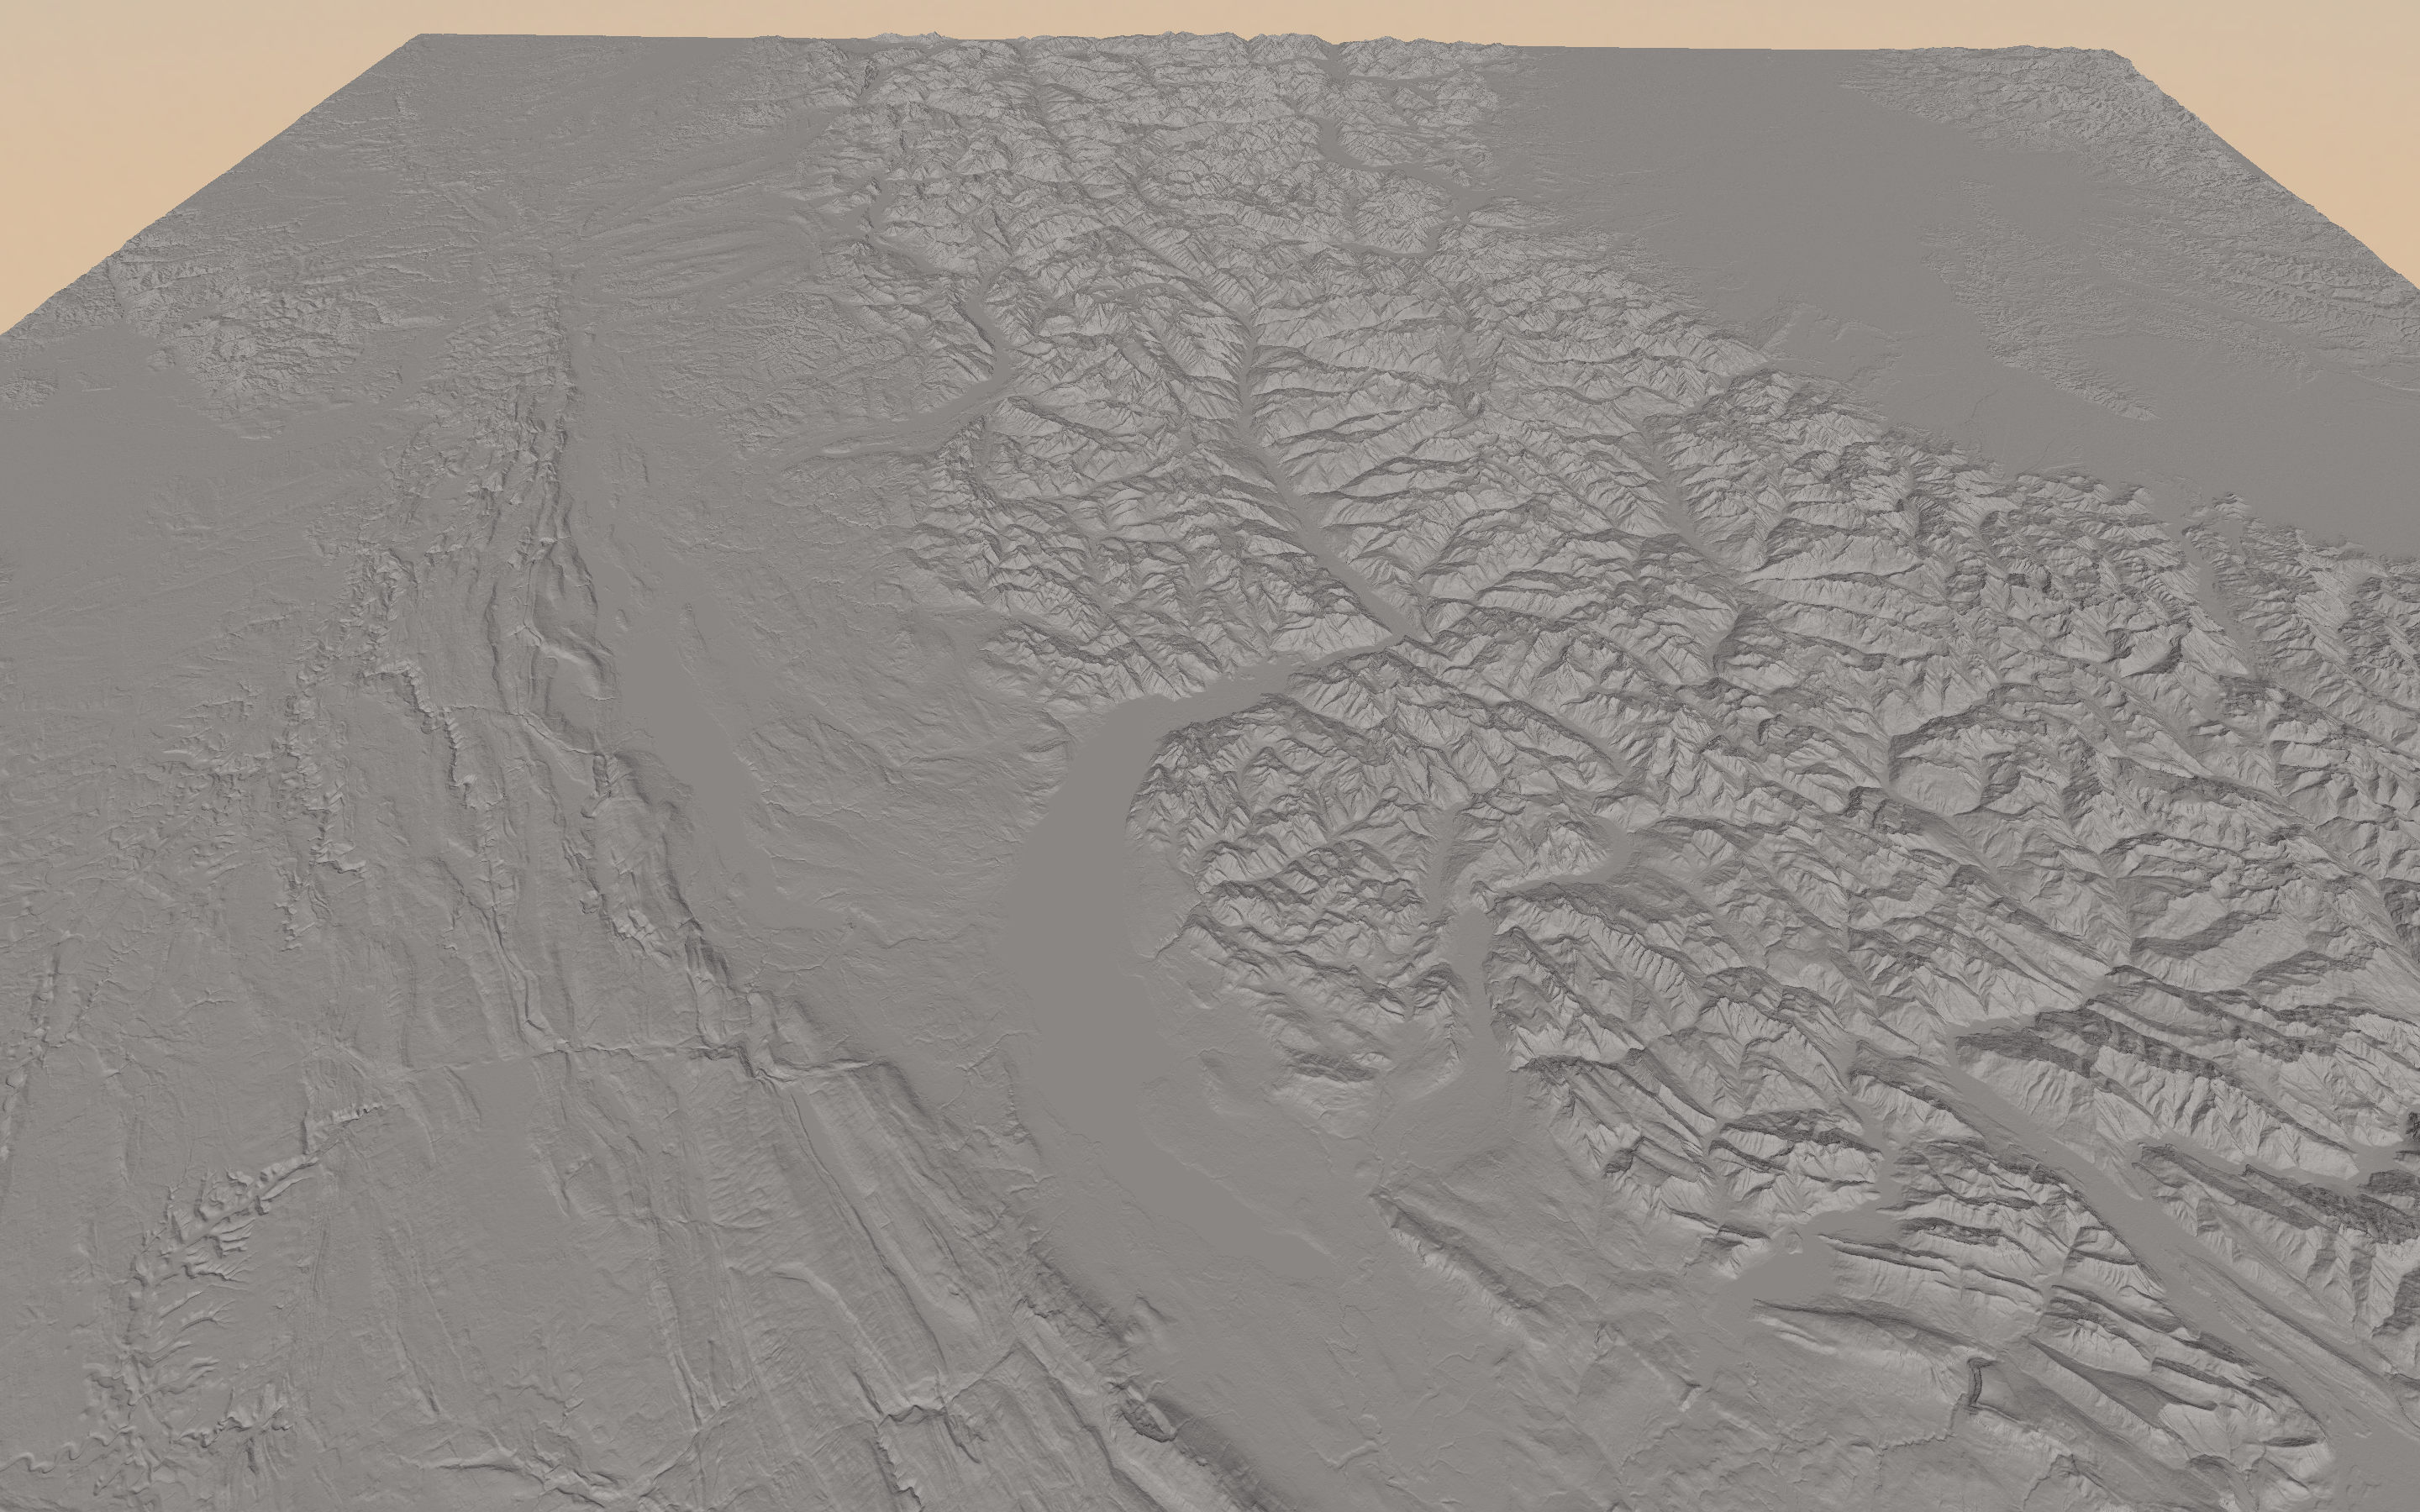
\includegraphics[width=0.4\textwidth]{results-accuracy-large-1-no-lod} }}
  \qquad
  \subfloat[\centering With LOD.]{{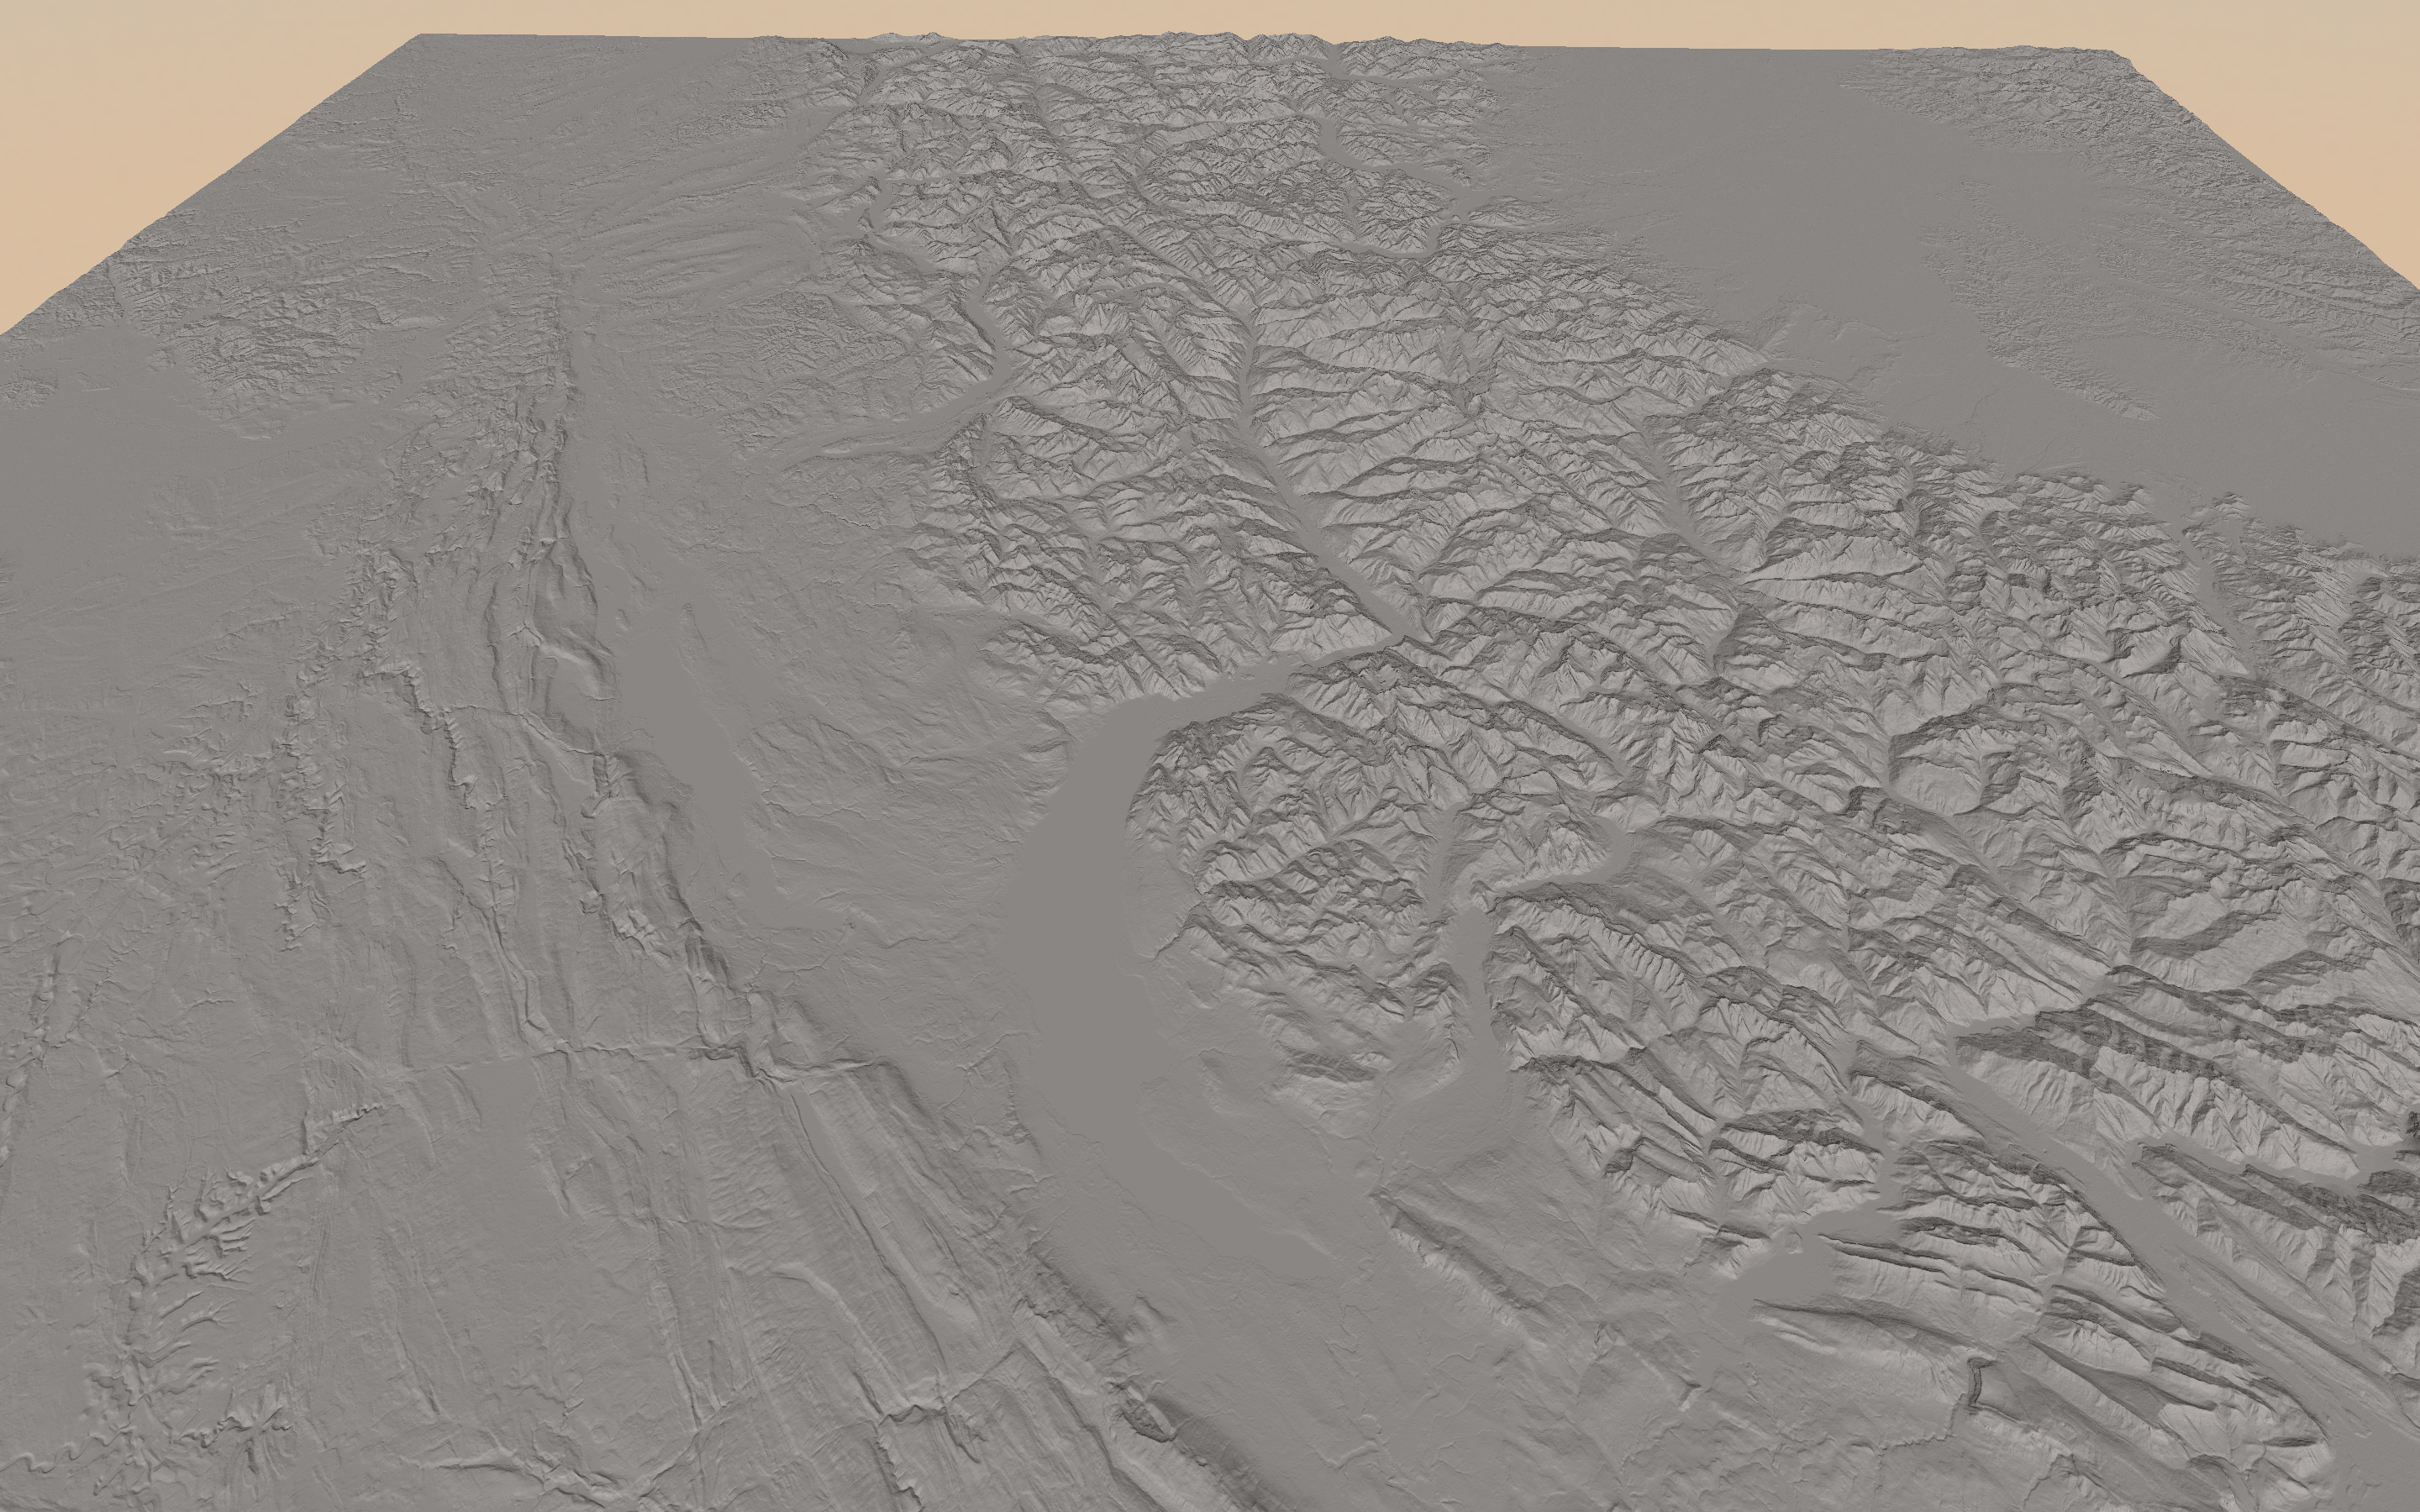
\includegraphics[width=0.4\textwidth]{results-accuracy-large-1-lod} }}
  \qquad
  \subfloat[\centering Absolute difference.]{{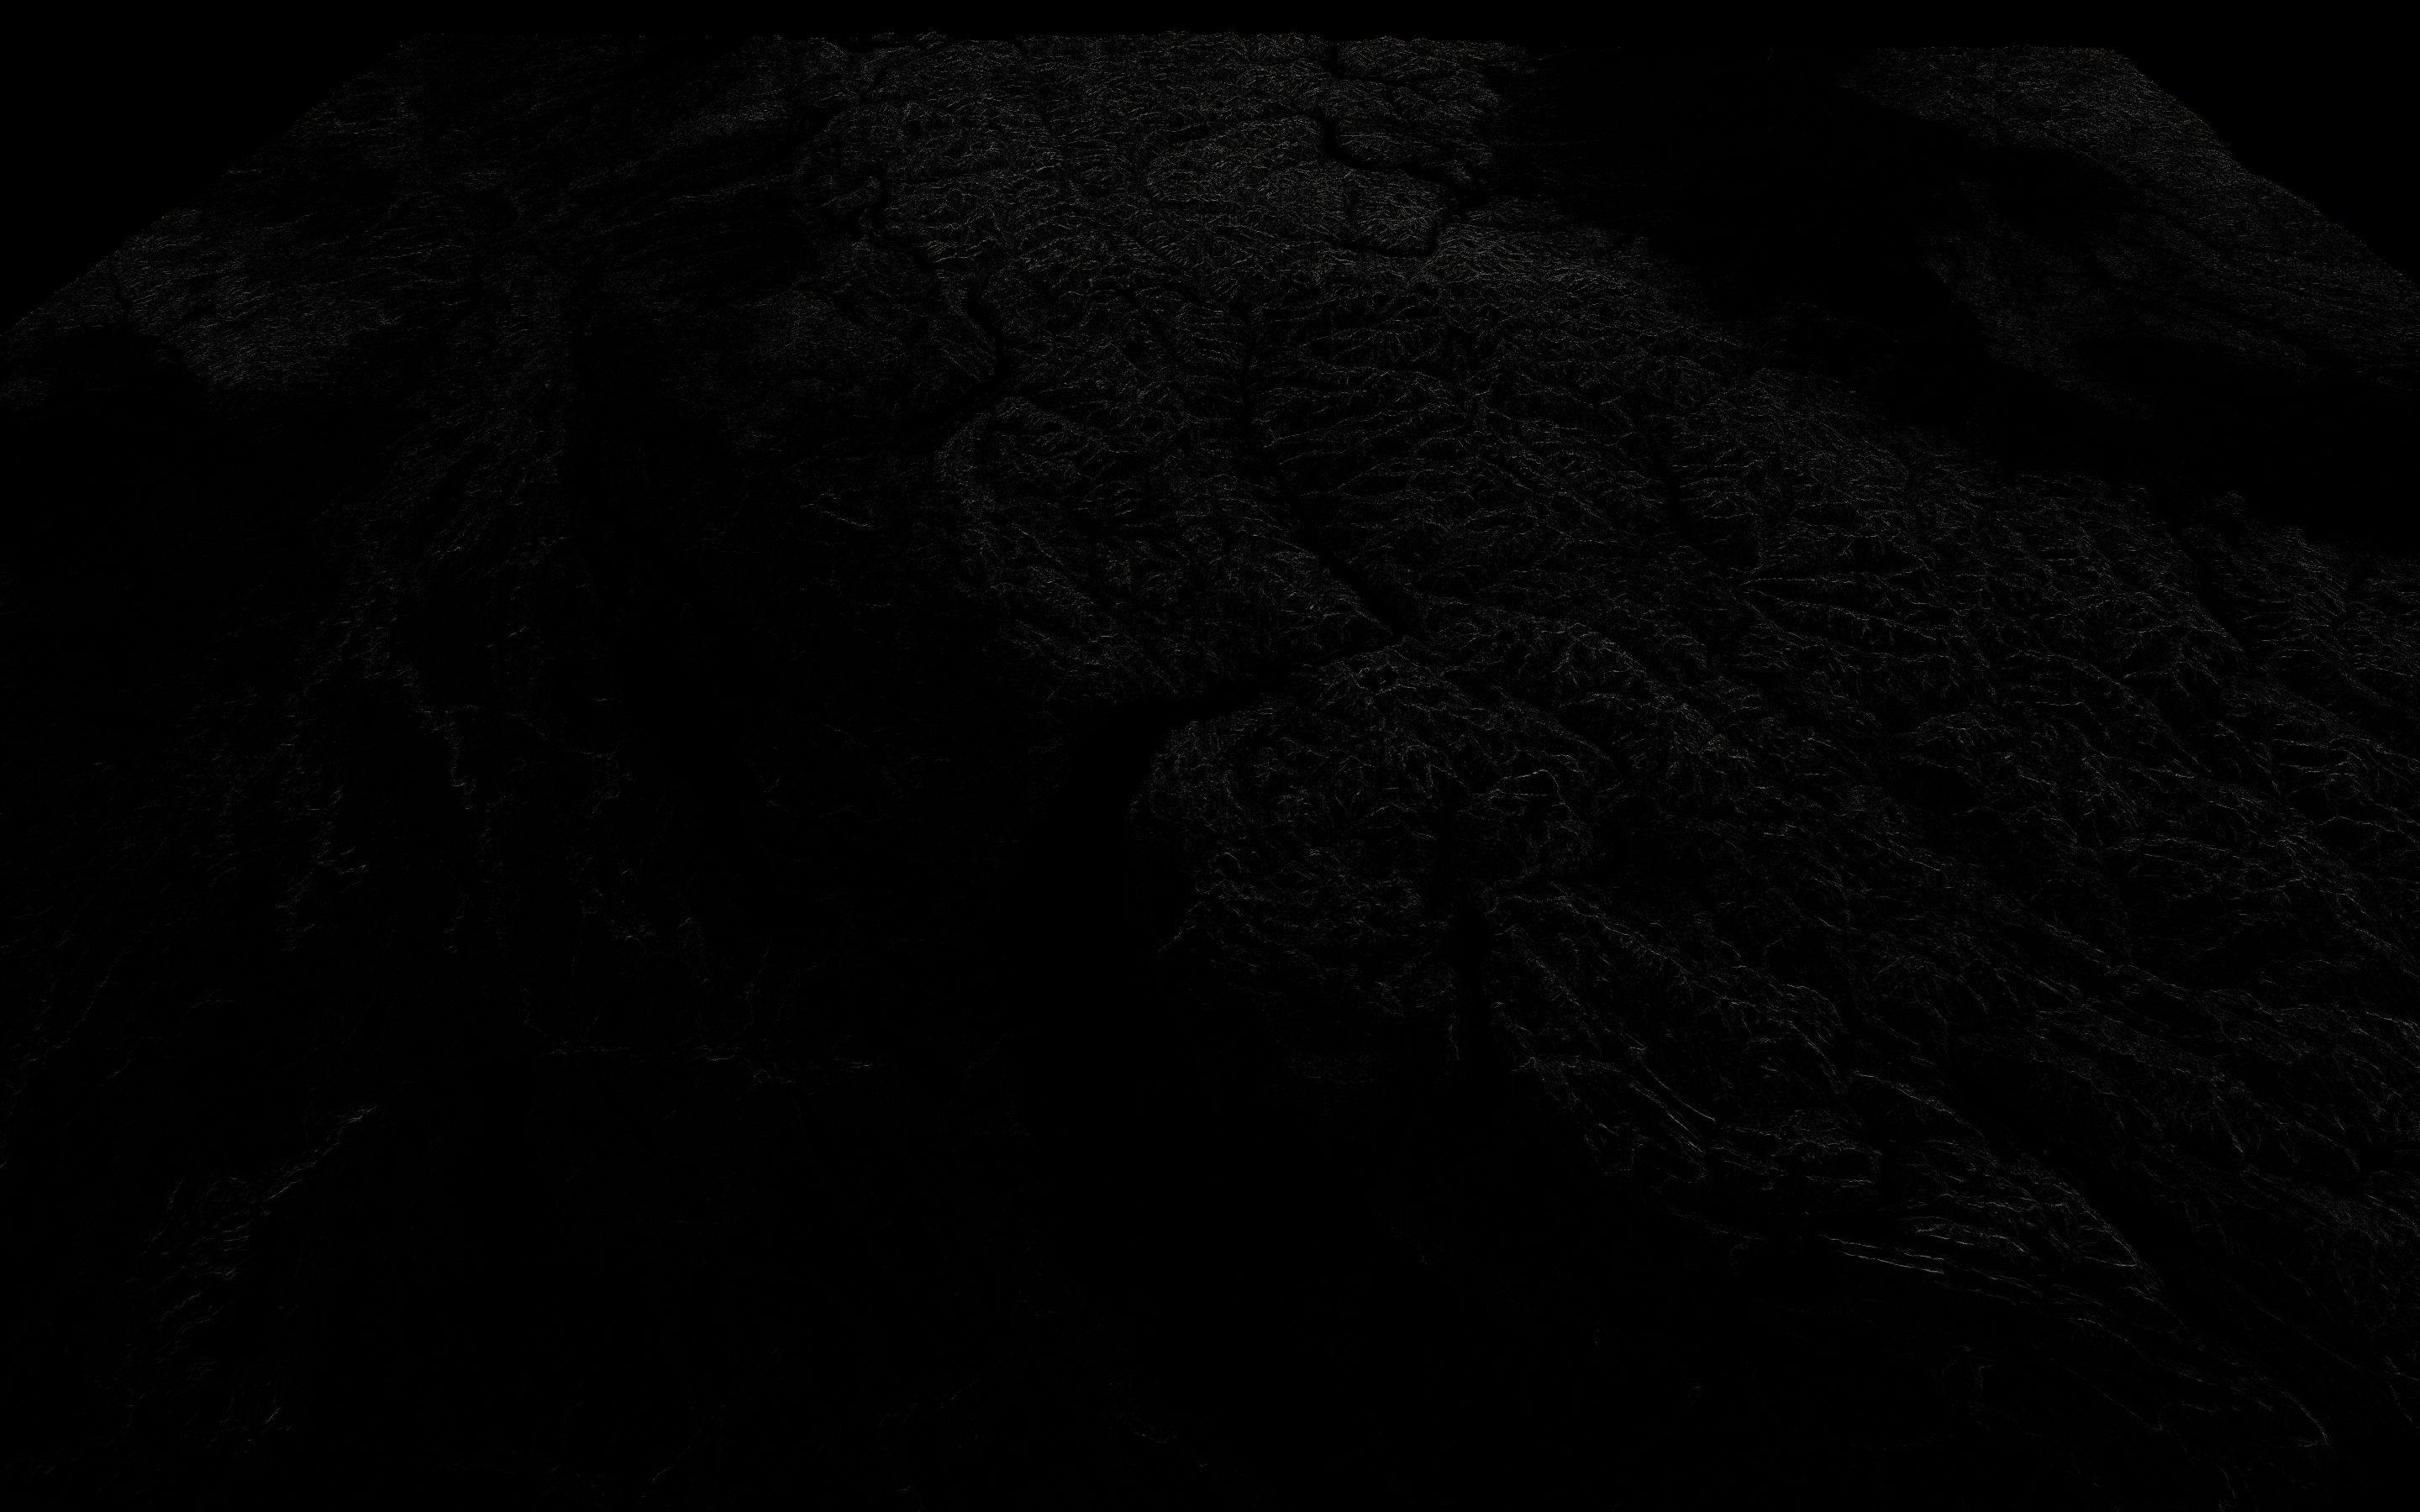
\includegraphics[width=0.4\textwidth]{results-accuracy-large-1-diff} }}
  \qquad
  \subfloat[\centering Absolute difference (binarised).]{{\includegraphics[width=0.4\textwidth]{results-accuracy-large-1-diff-bin} }}
  \caption{Screenshot showcasing the screenshot of a large section of the terrain with no LOD (a), with LOD (b),
   the absolute difference (c) between (a) and (b), and the binarised absolute difference (d) of (c). The computed RMSE is 3.94.}\label{fig:results-large-1}
\end{figure}
\subsubsection{Large Terrain Screenshot 2}
\begin{figure}[H]
  \centering
  \subfloat[\centering No LOD.]{{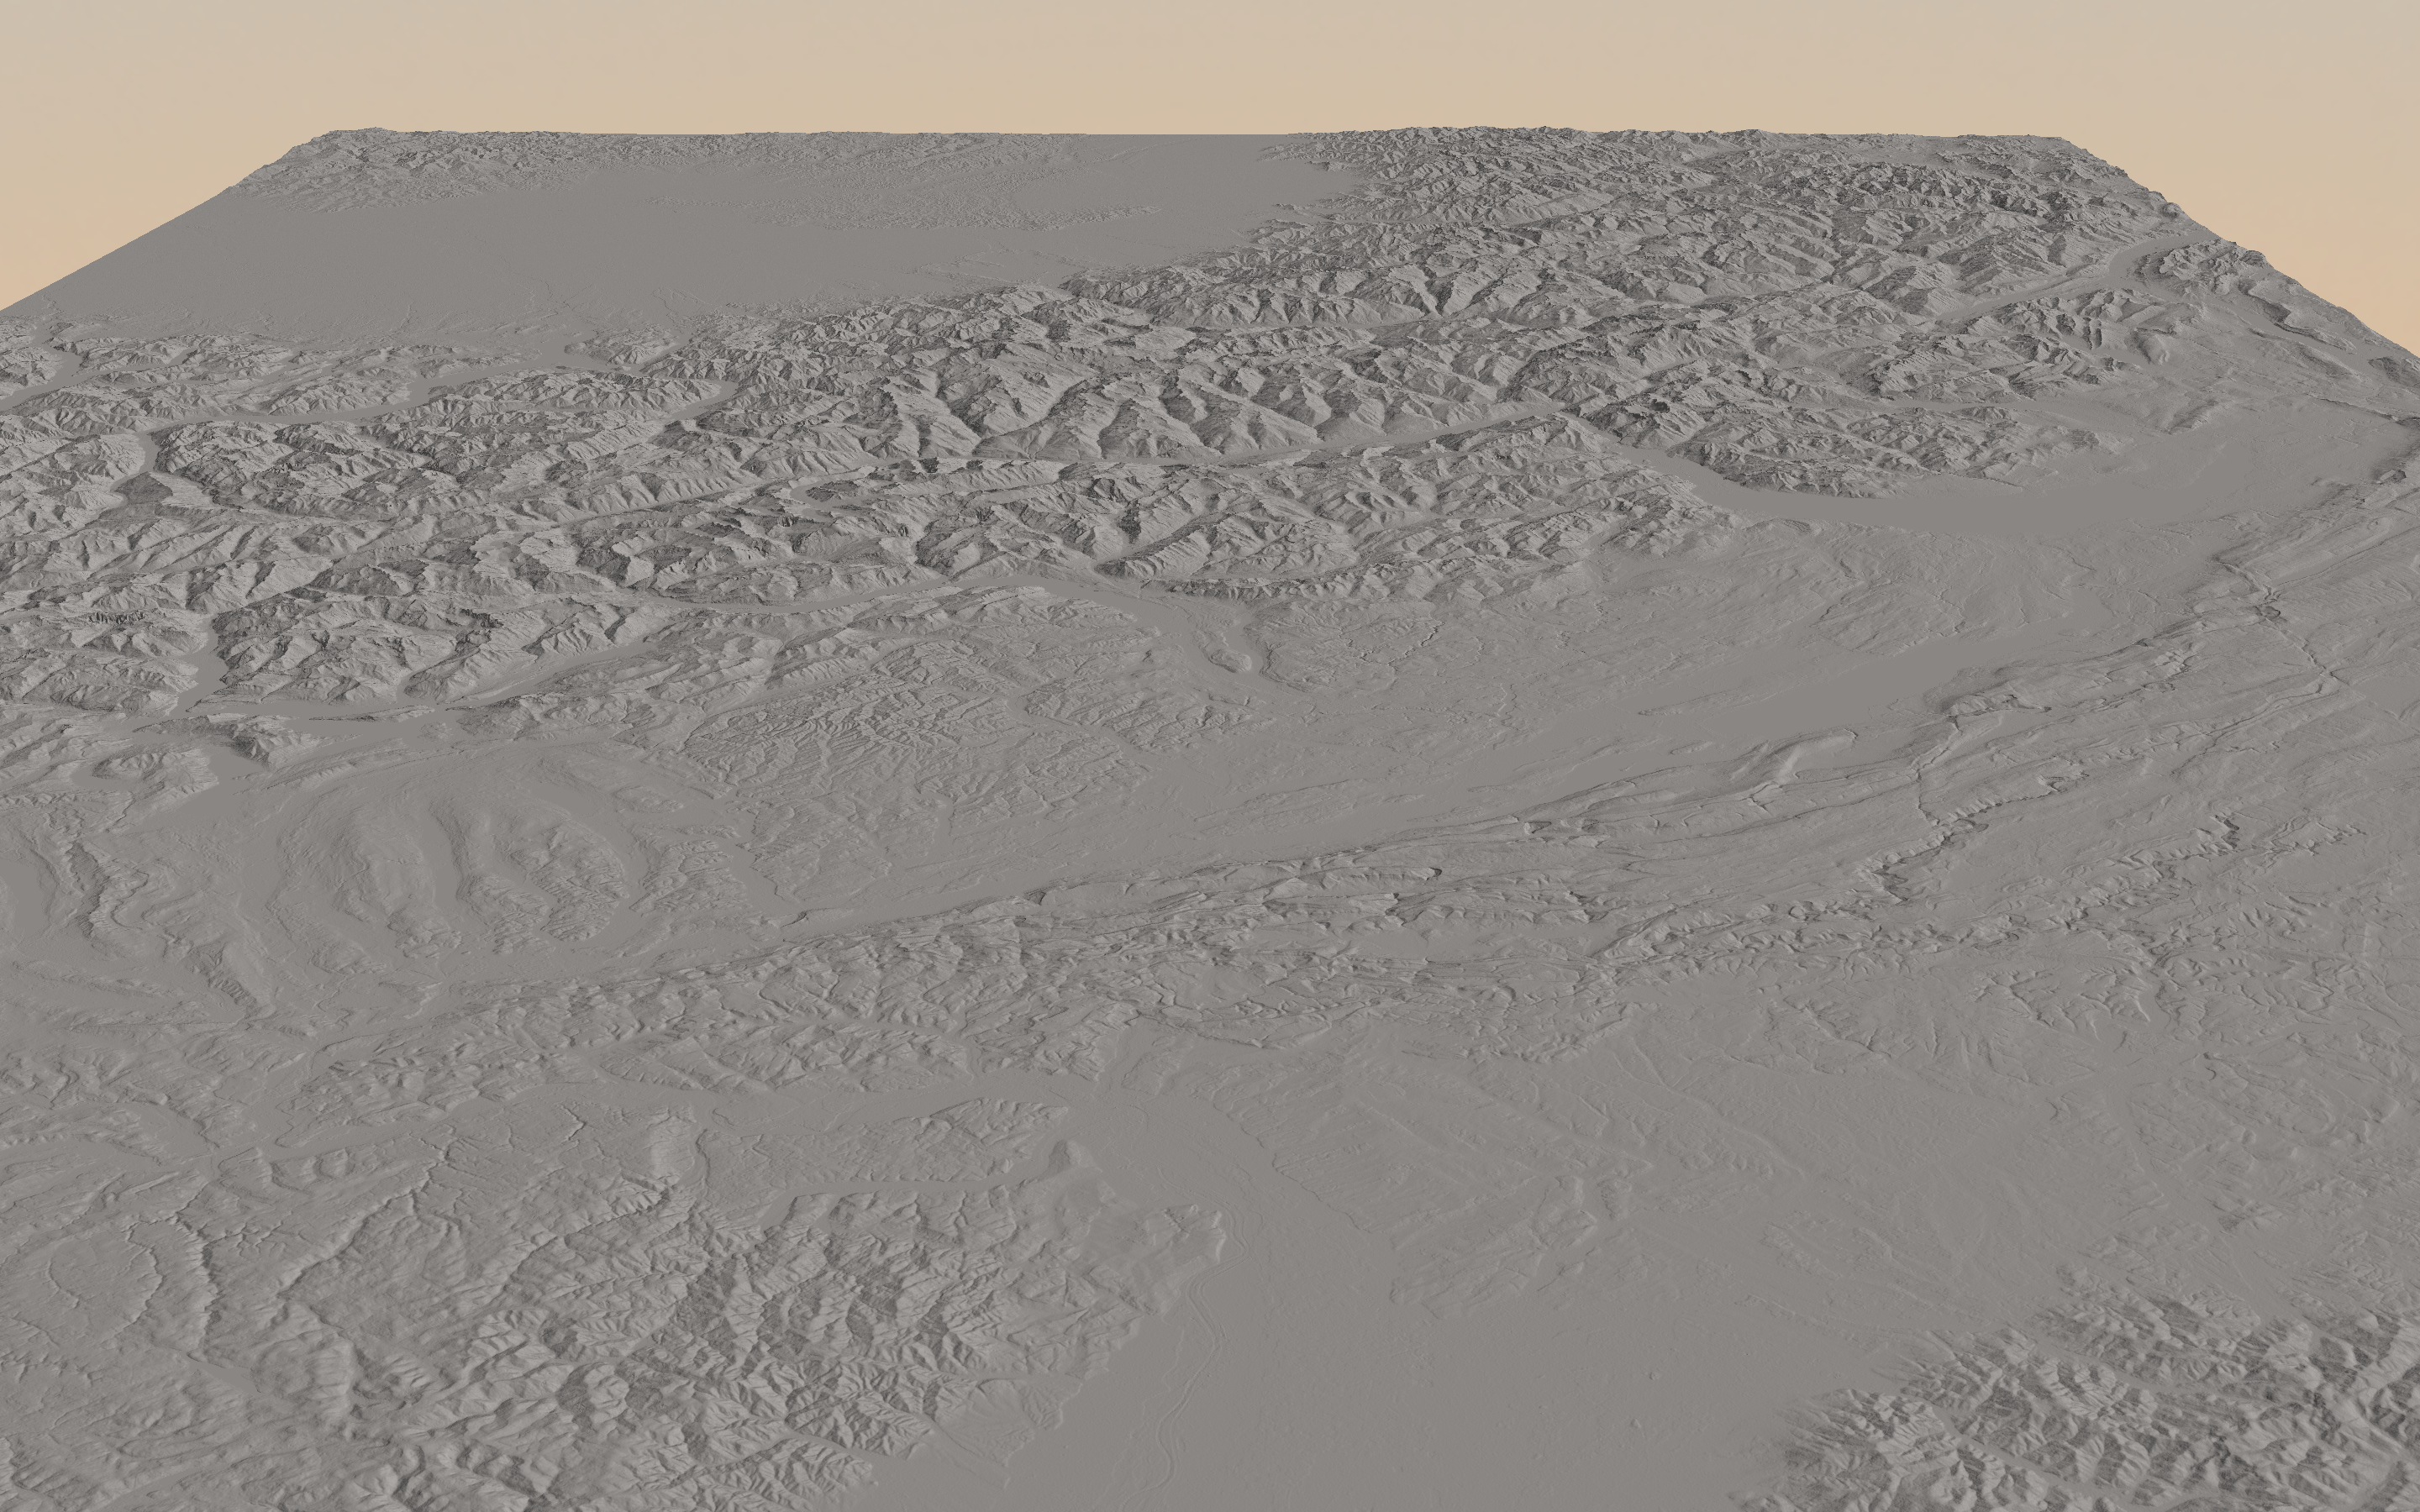
\includegraphics[width=0.4\textwidth]{results-accuracy-large-2-no-lod} }}
  \qquad
  \subfloat[\centering With LOD.]{{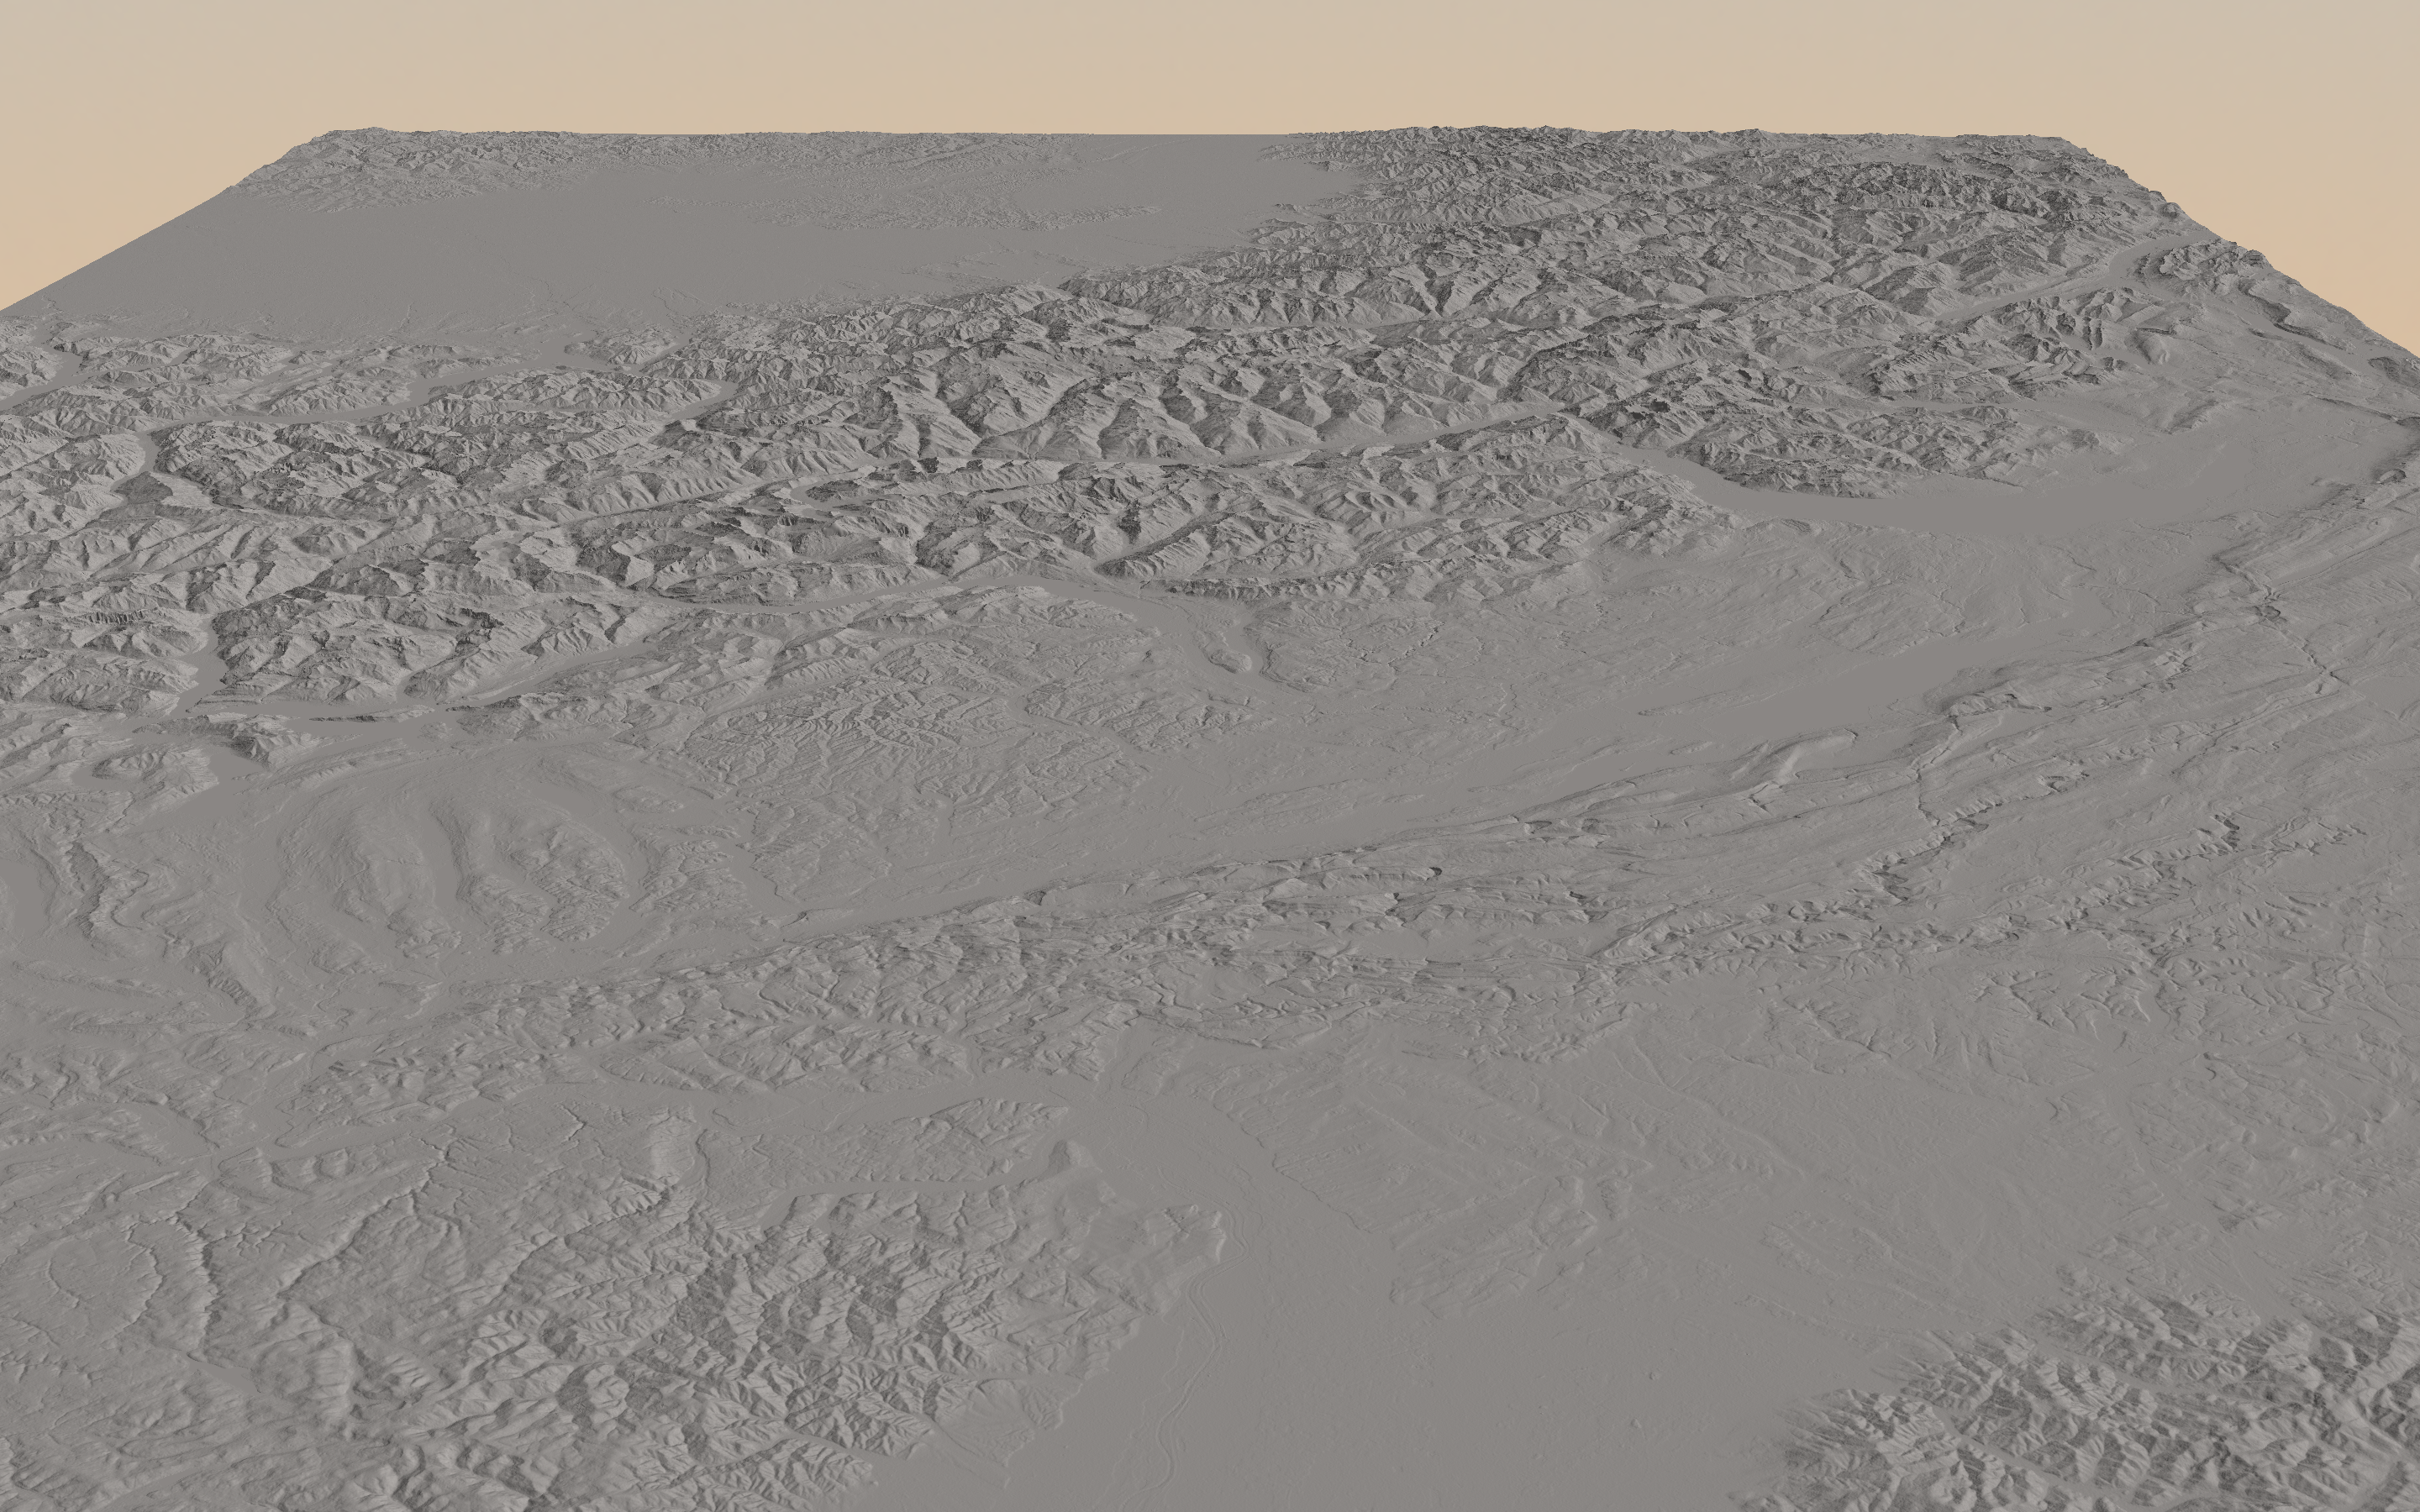
\includegraphics[width=0.4\textwidth]{results-accuracy-large-2-lod} }}
  \qquad
  \subfloat[\centering Absolute difference.]{{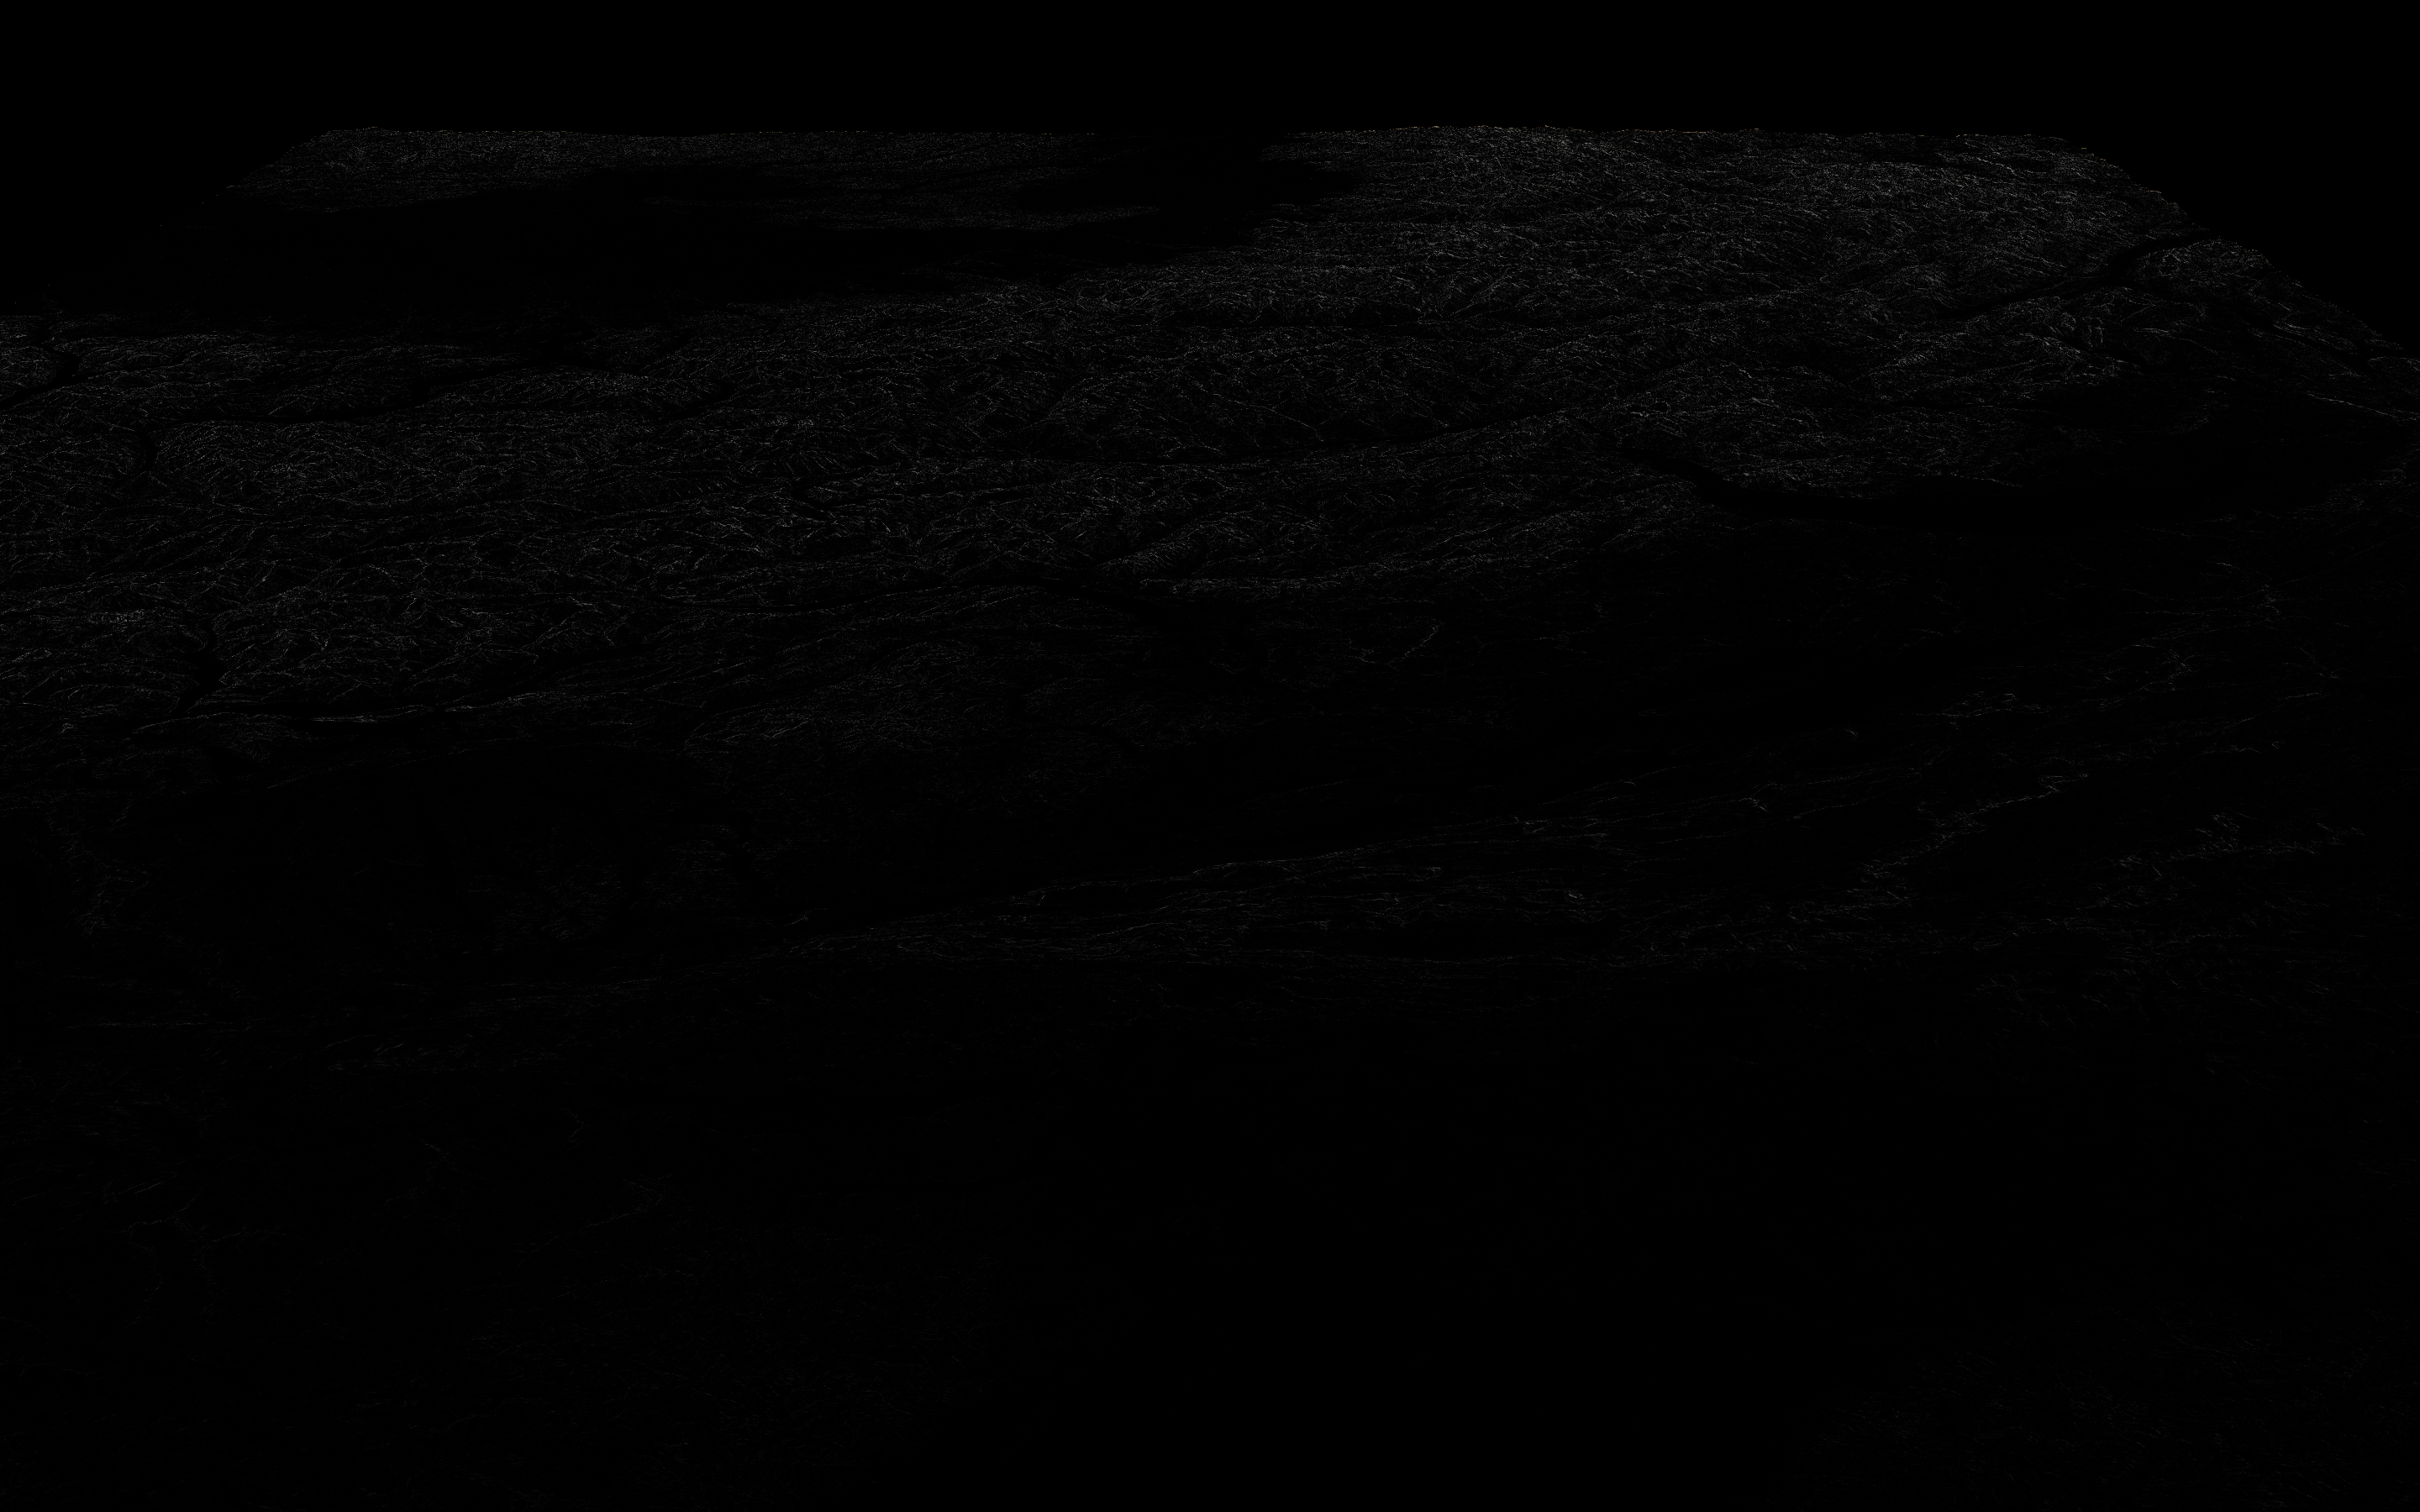
\includegraphics[width=0.4\textwidth]{results-accuracy-large-2-diff} }}
  \qquad
  \subfloat[\centering Absolute difference (binarised).]{{\includegraphics[width=0.4\textwidth]{results-accuracy-large-2-diff-bin} }}
  \caption{Screenshot showcasing the screenshot of a large section of the terrain with no LOD (a), with LOD (b),
   the absolute difference (c) between (a) and (b), and the binarised absolute difference (d) of (c). The computed RMSE is 3.1.}\label{fig:results-large-2}
\end{figure}
\subsubsection{Large Terrain Screenshot 3}
\begin{figure}[H]
  \centering
  \subfloat[\centering No LOD.]{{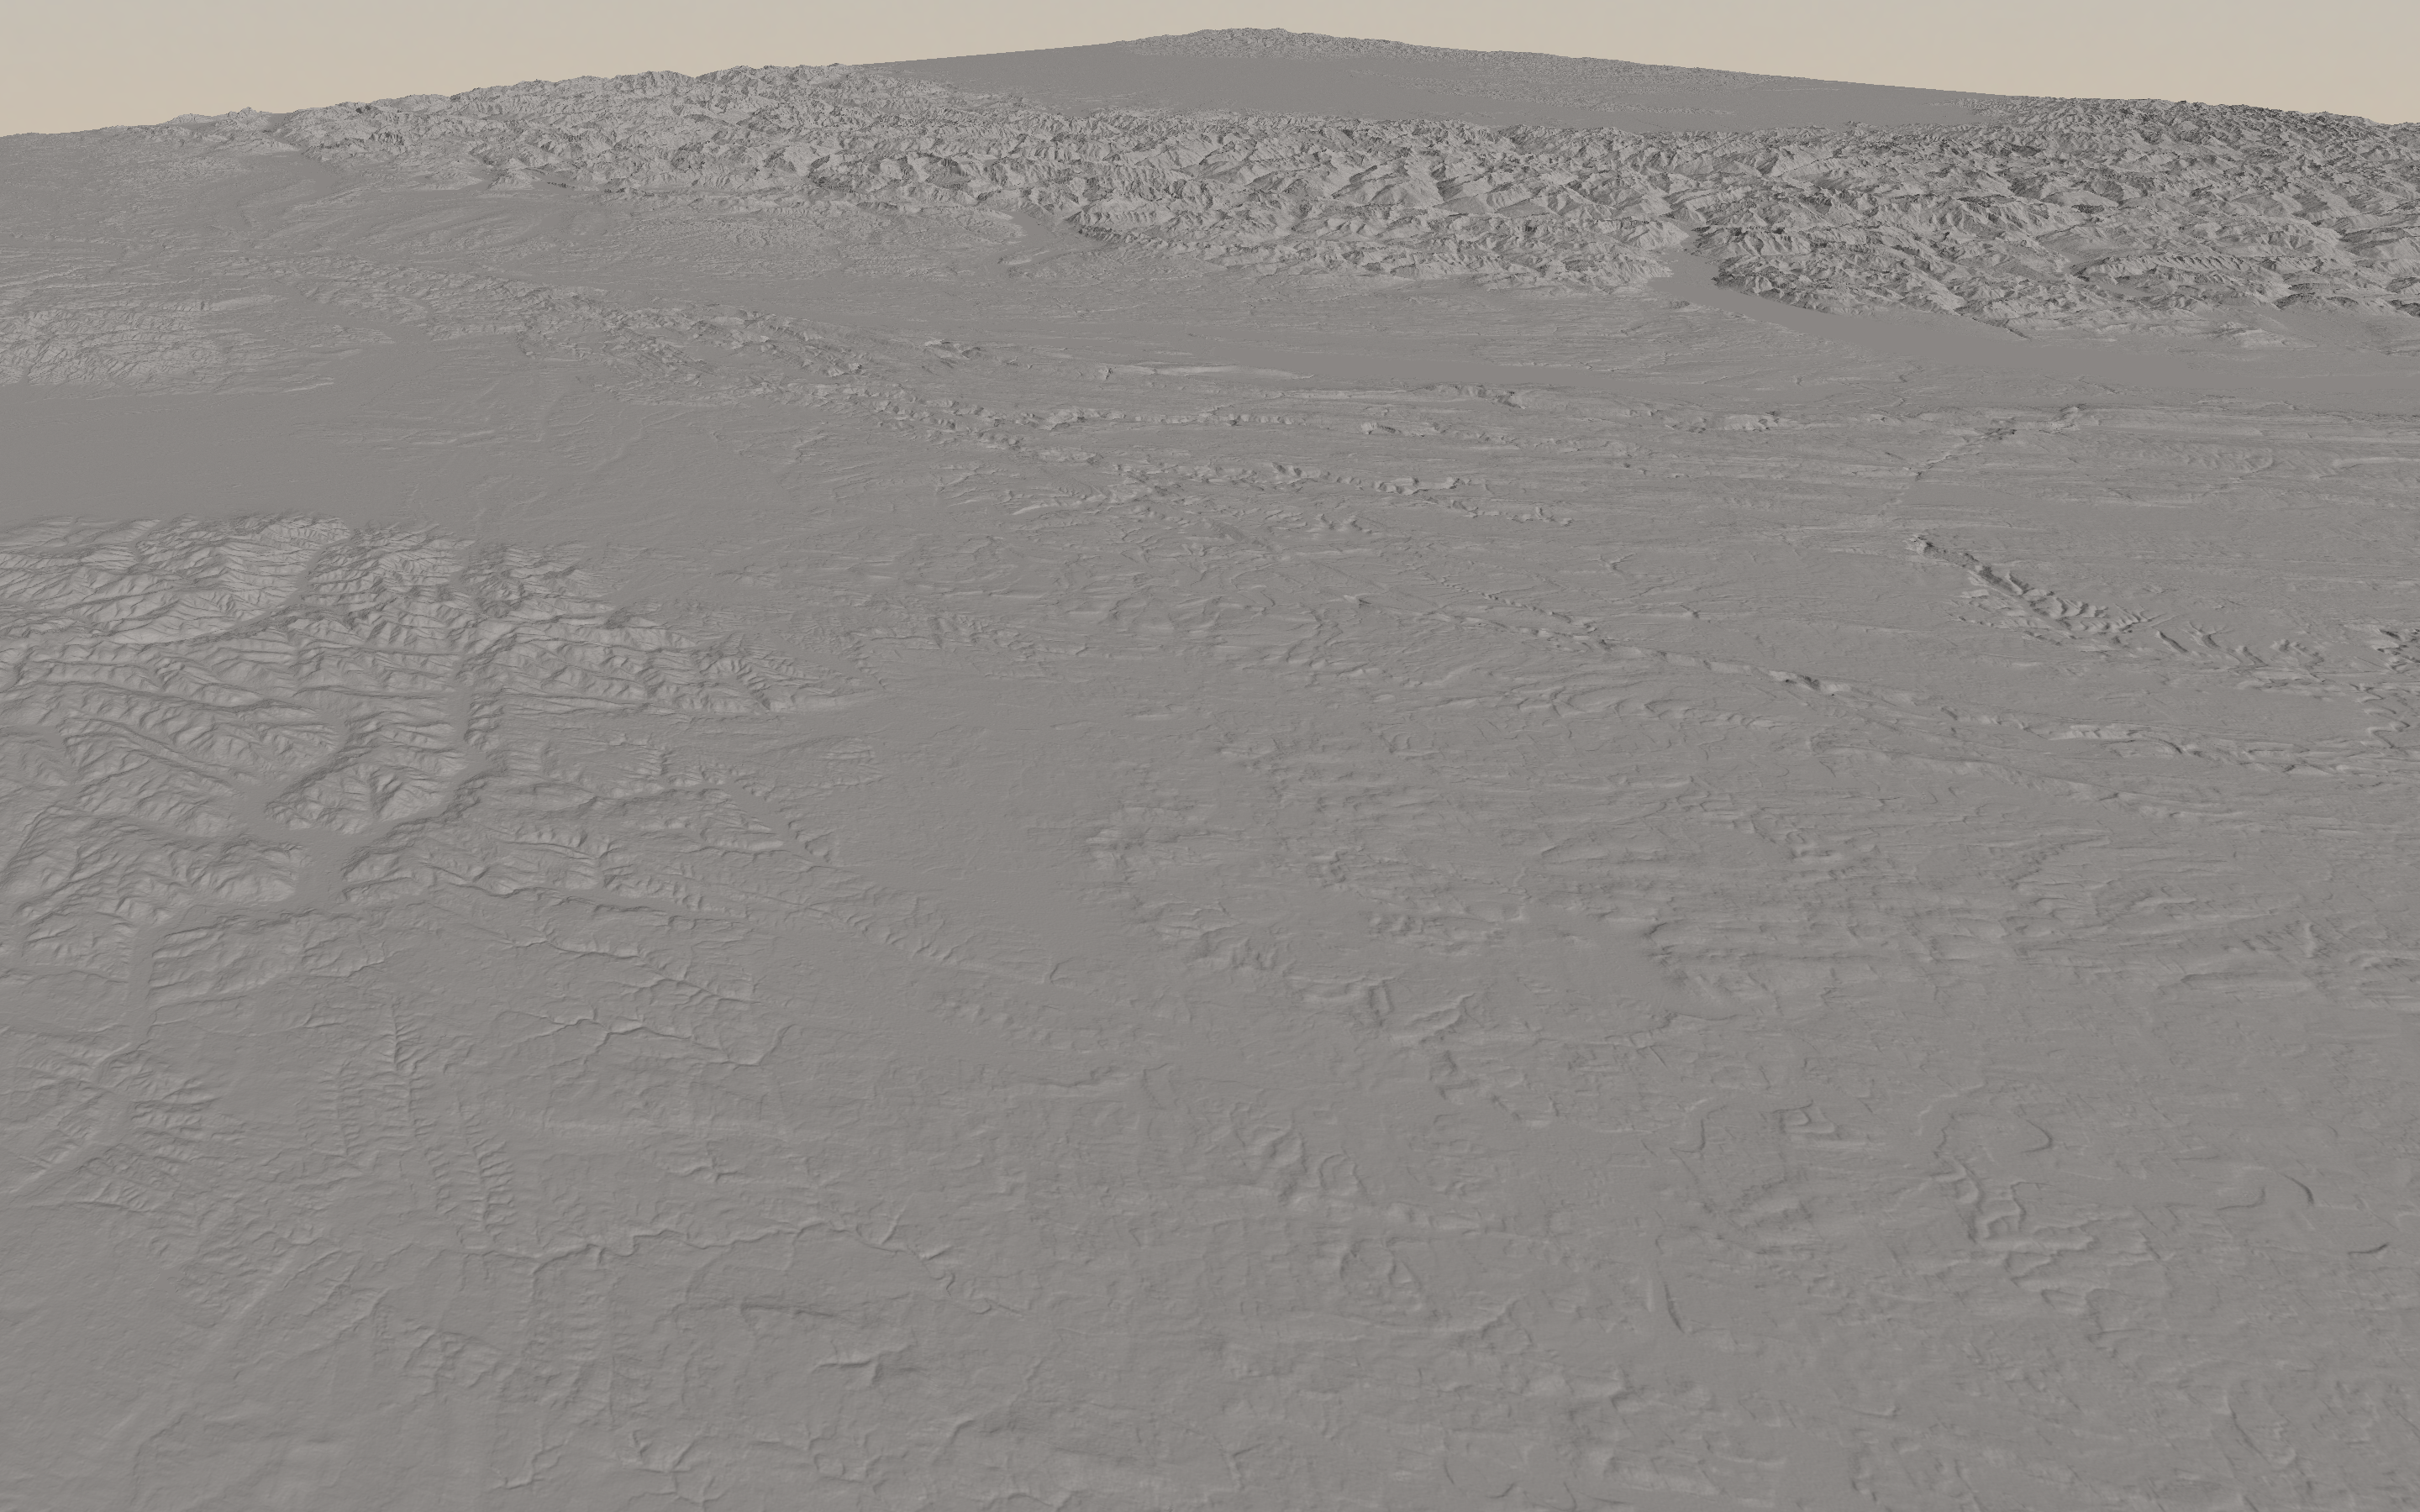
\includegraphics[width=0.4\textwidth]{results-accuracy-large-3-no-lod} }}
  \qquad
  \subfloat[\centering With LOD.]{{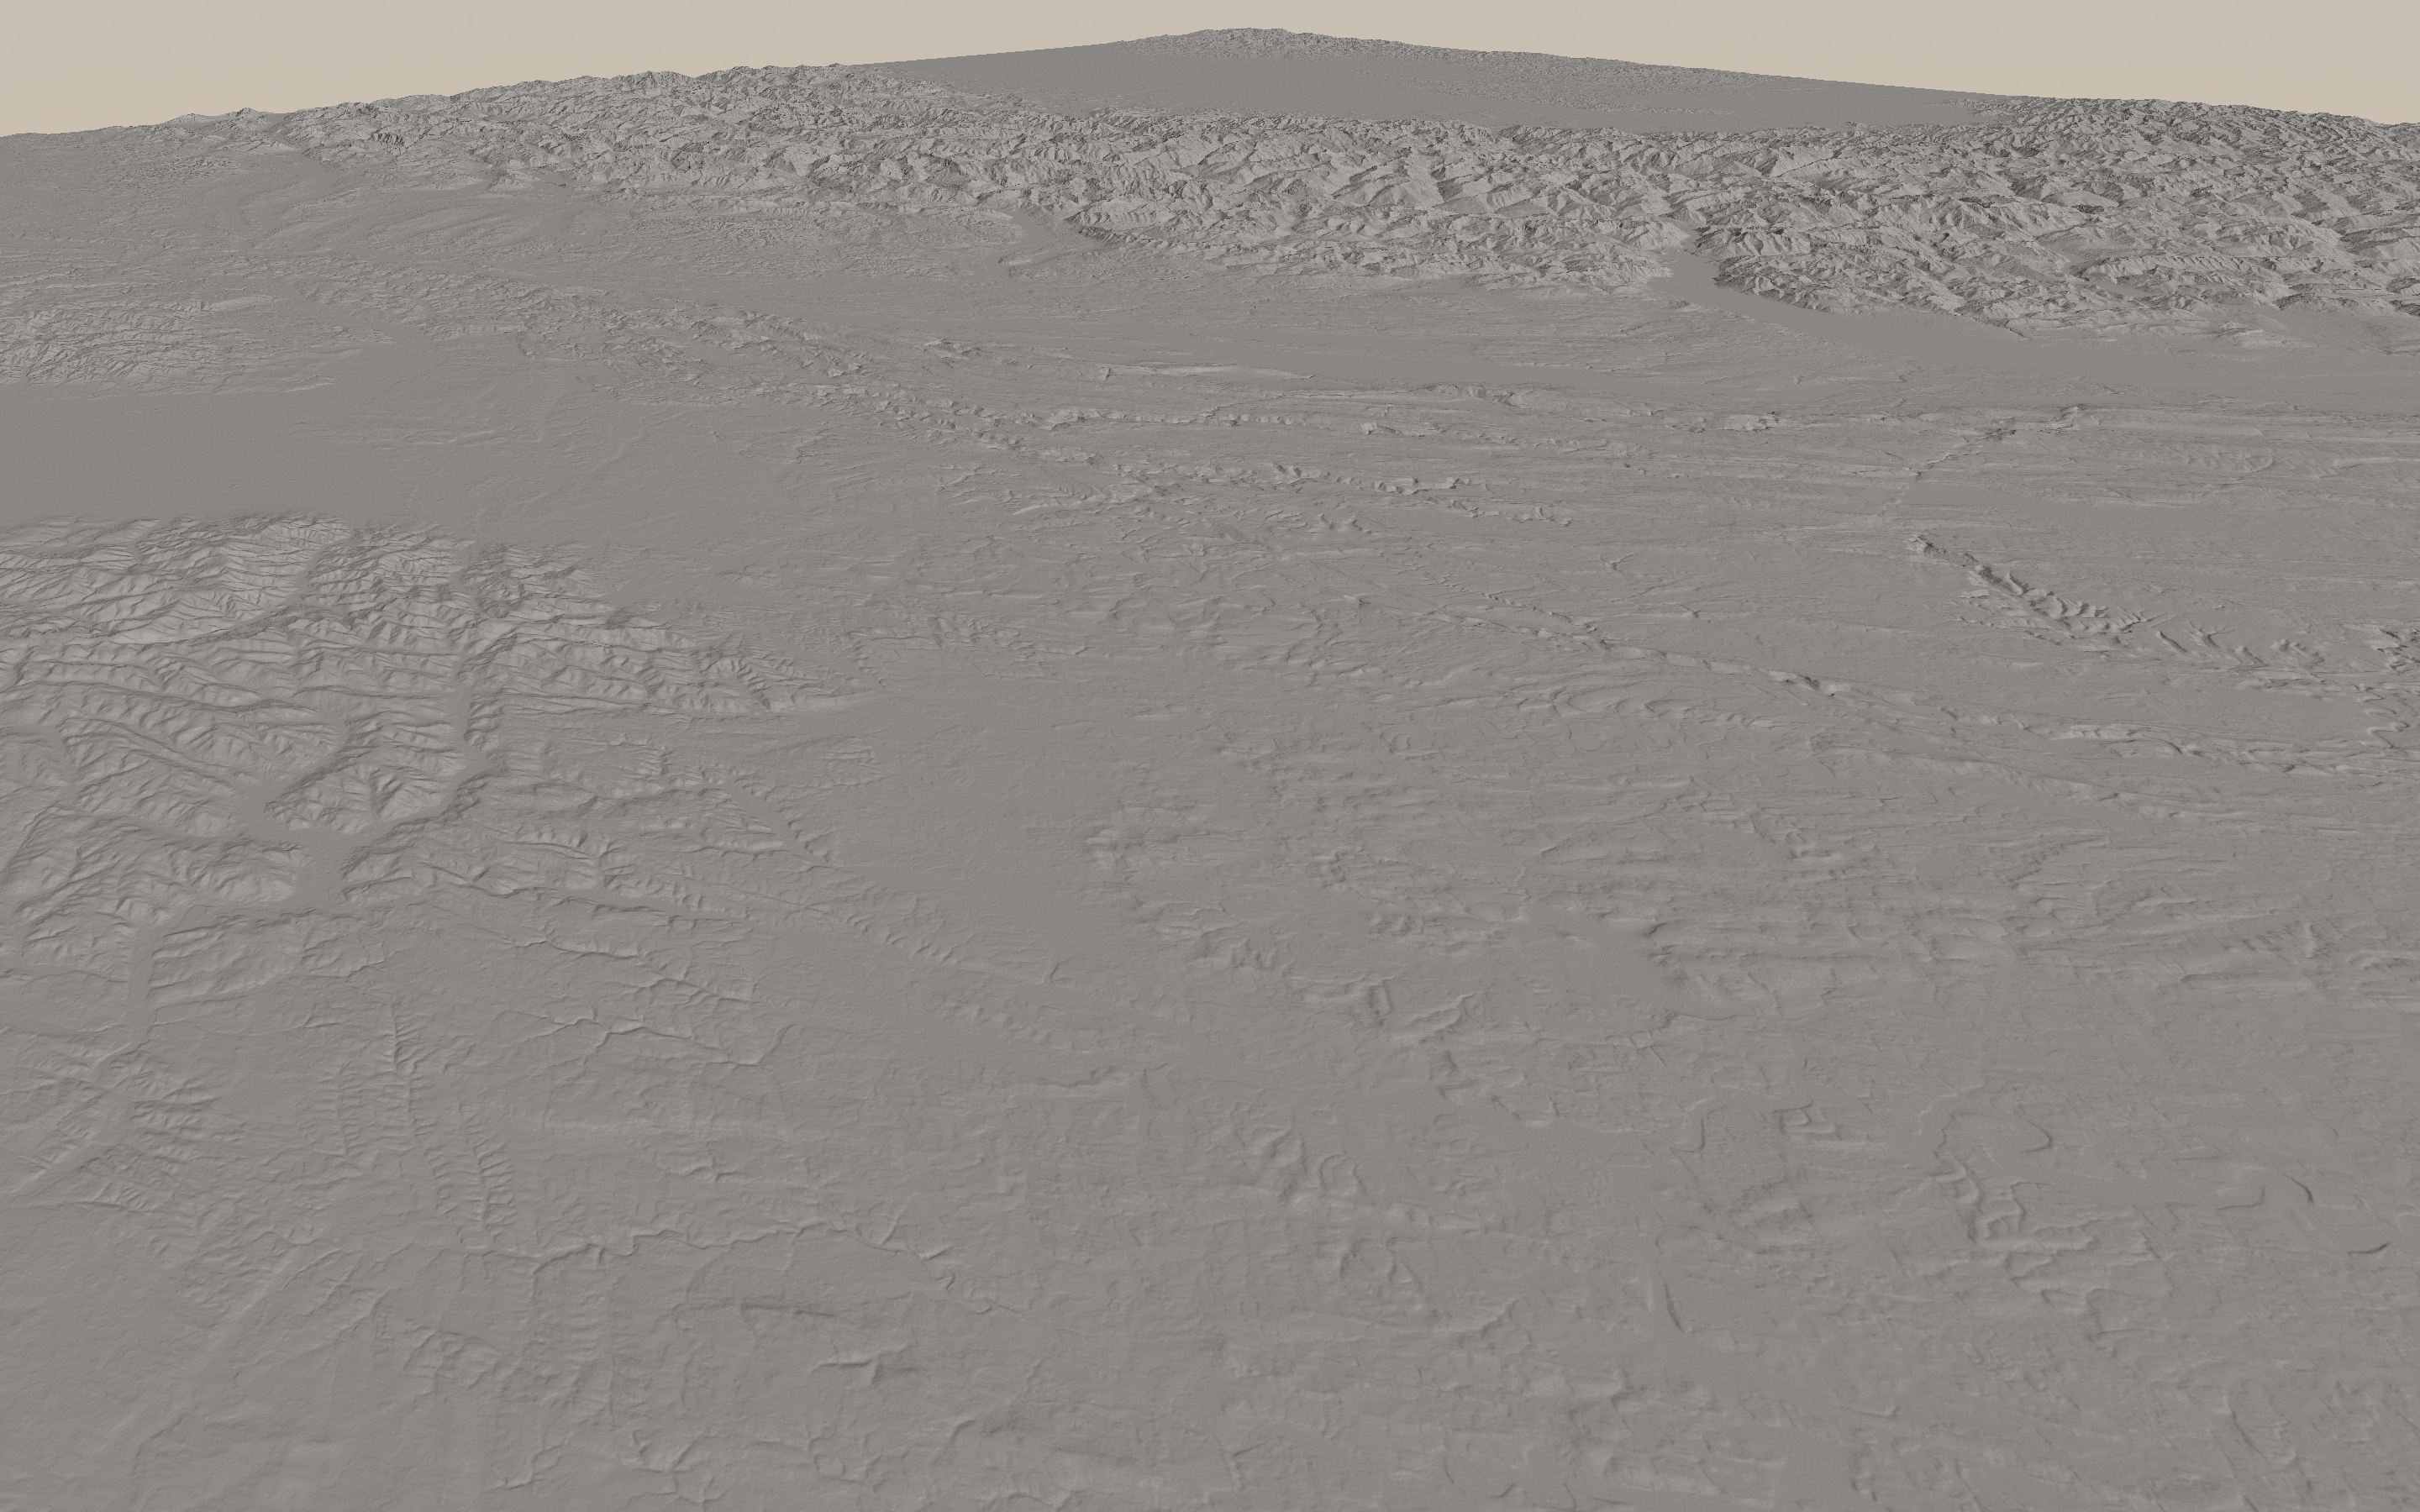
\includegraphics[width=0.4\textwidth]{results-accuracy-large-3-lod} }}
  \qquad
  \subfloat[\centering Absolute difference.]{{\includegraphics[width=0.4\textwidth]{results-accuracy-large-3-diff} }}
  \qquad
  \subfloat[\centering Absolute difference (binarised).]{{\includegraphics[width=0.4\textwidth]{results-accuracy-large-3-diff-bin} }}
  \caption{Screenshot showcasing the screenshot of a large section of the terrain with no LOD (a), with LOD (b),
   the absolute difference (c) between (a) and (b), and the binarised absolute difference (d) of (c). The computed RMSE is 2.59.}\label{fig:results-large-3}
\end{figure}
\subsubsection{Large Terrain Screenshot 4}
\begin{figure}[H]
  \centering
  \subfloat[\centering No LOD.]{{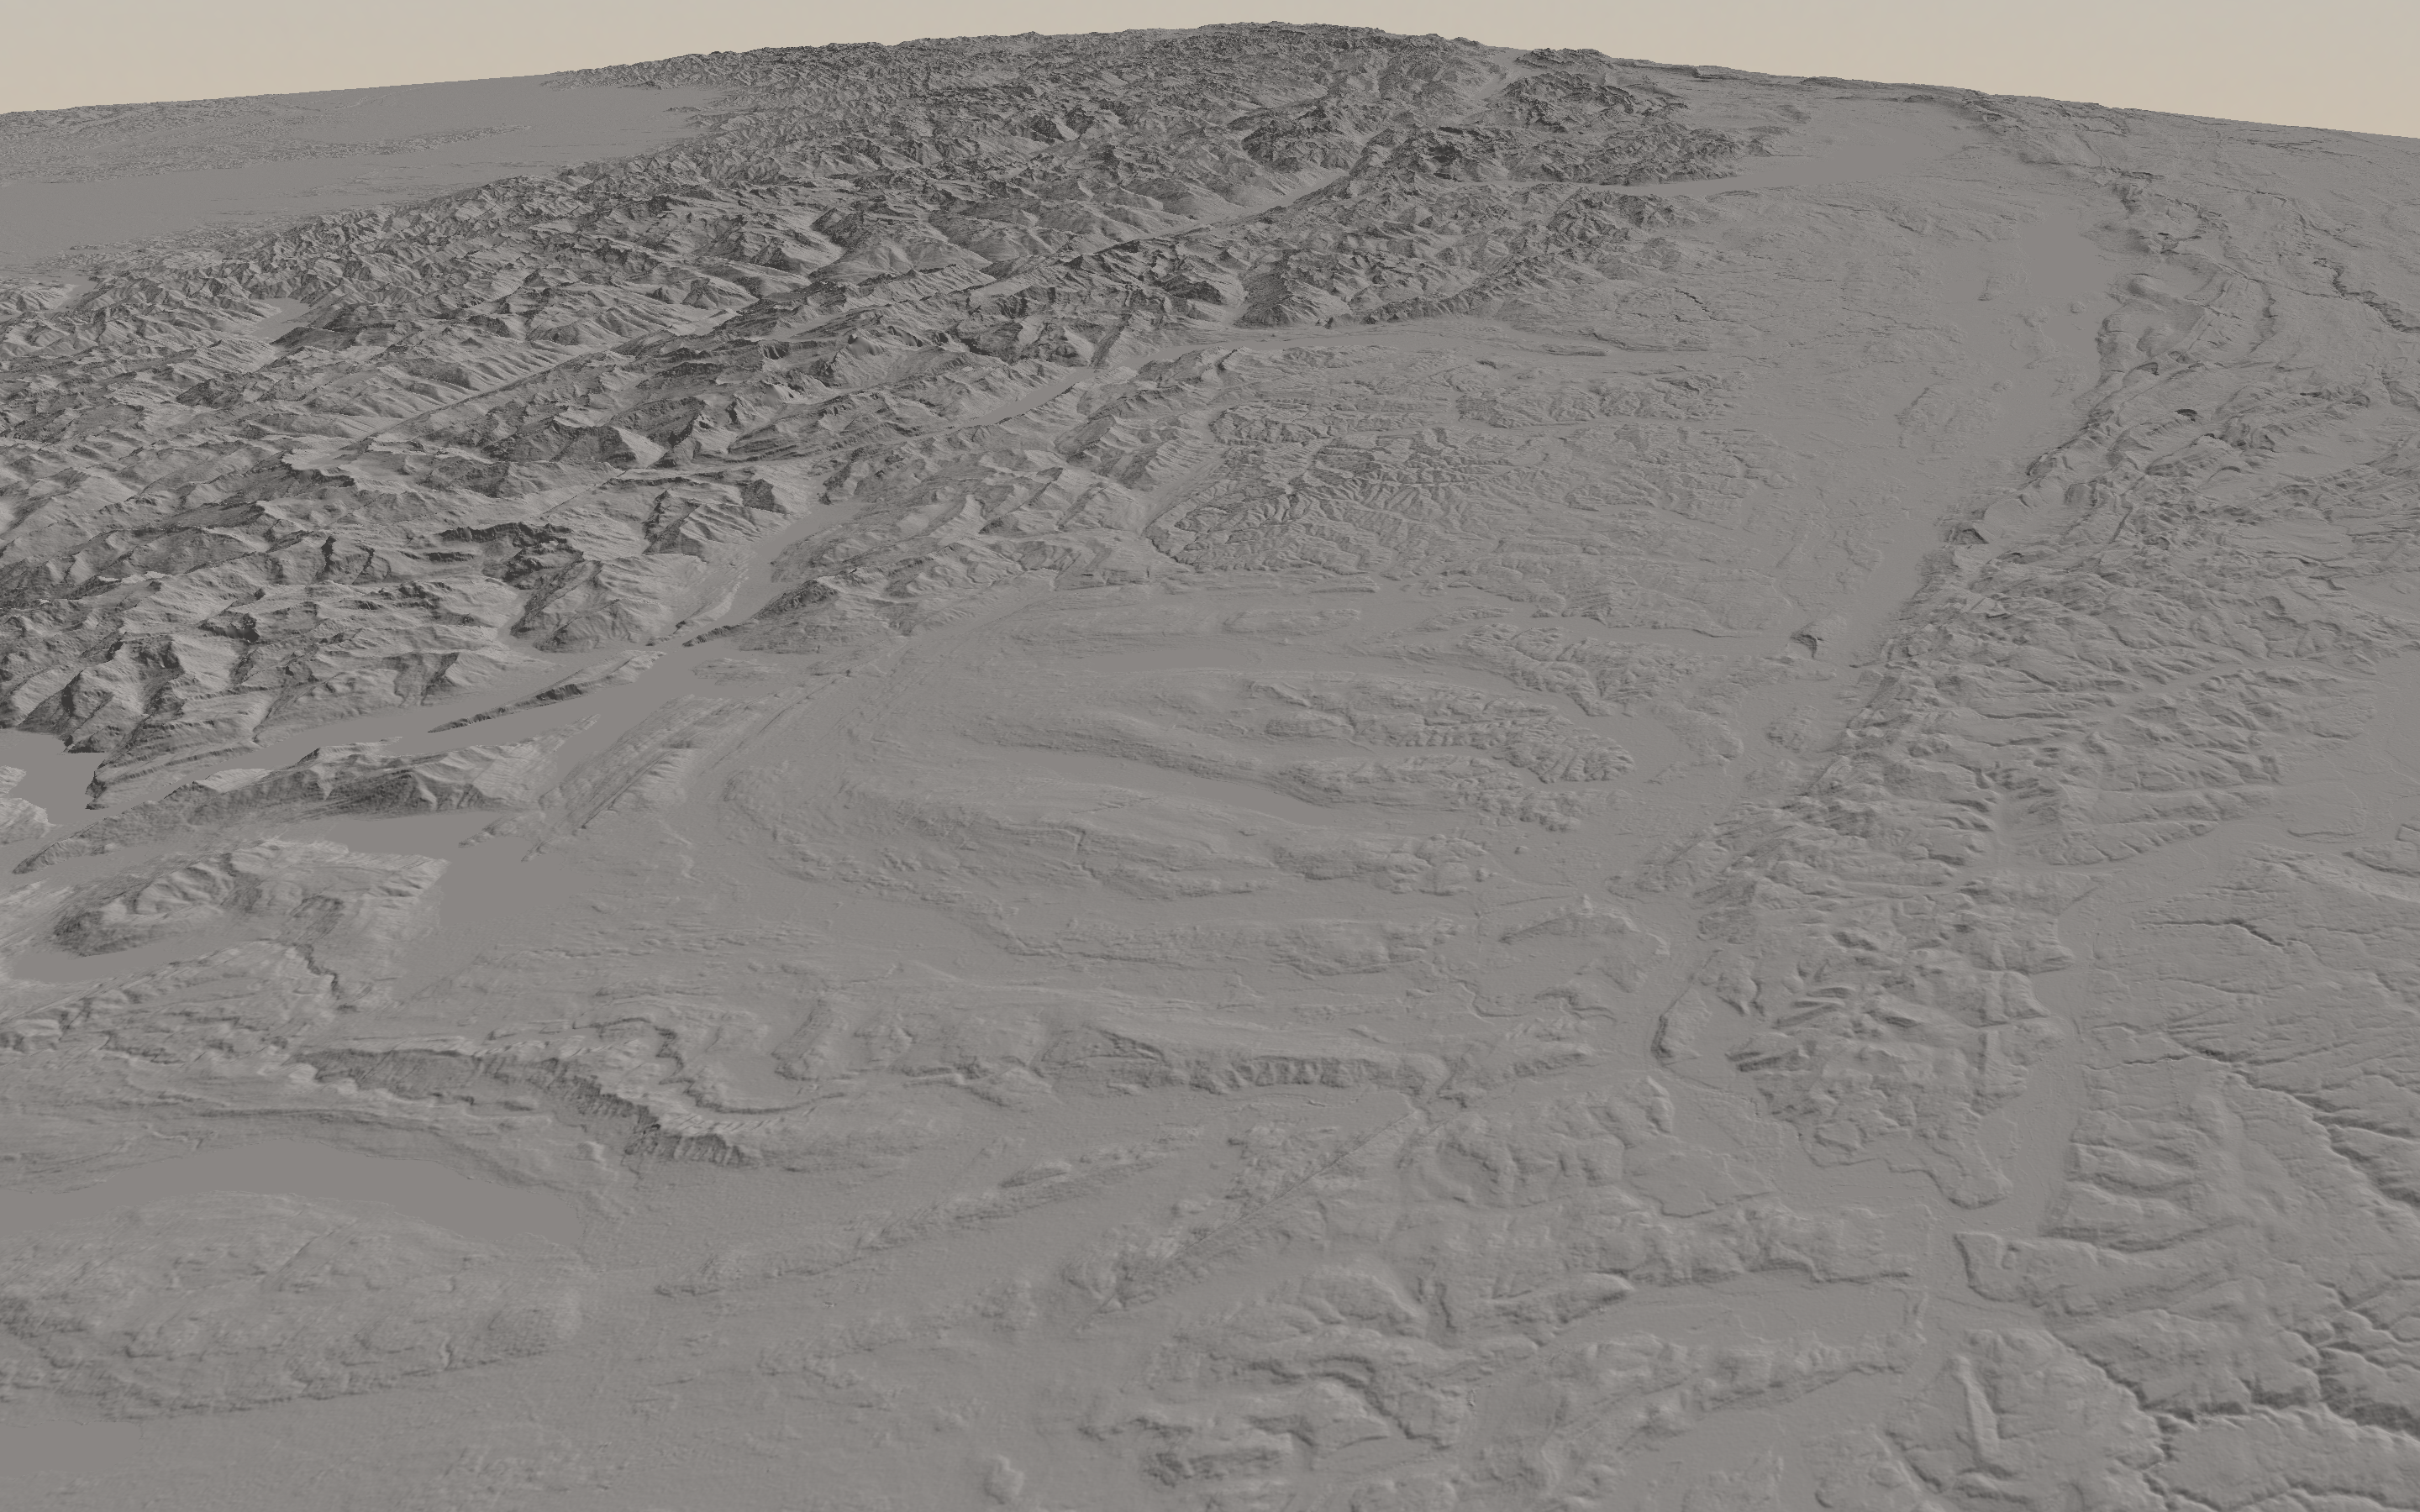
\includegraphics[width=0.4\textwidth]{results-accuracy-large-4-no-lod} }}
  \qquad
  \subfloat[\centering With LOD.]{{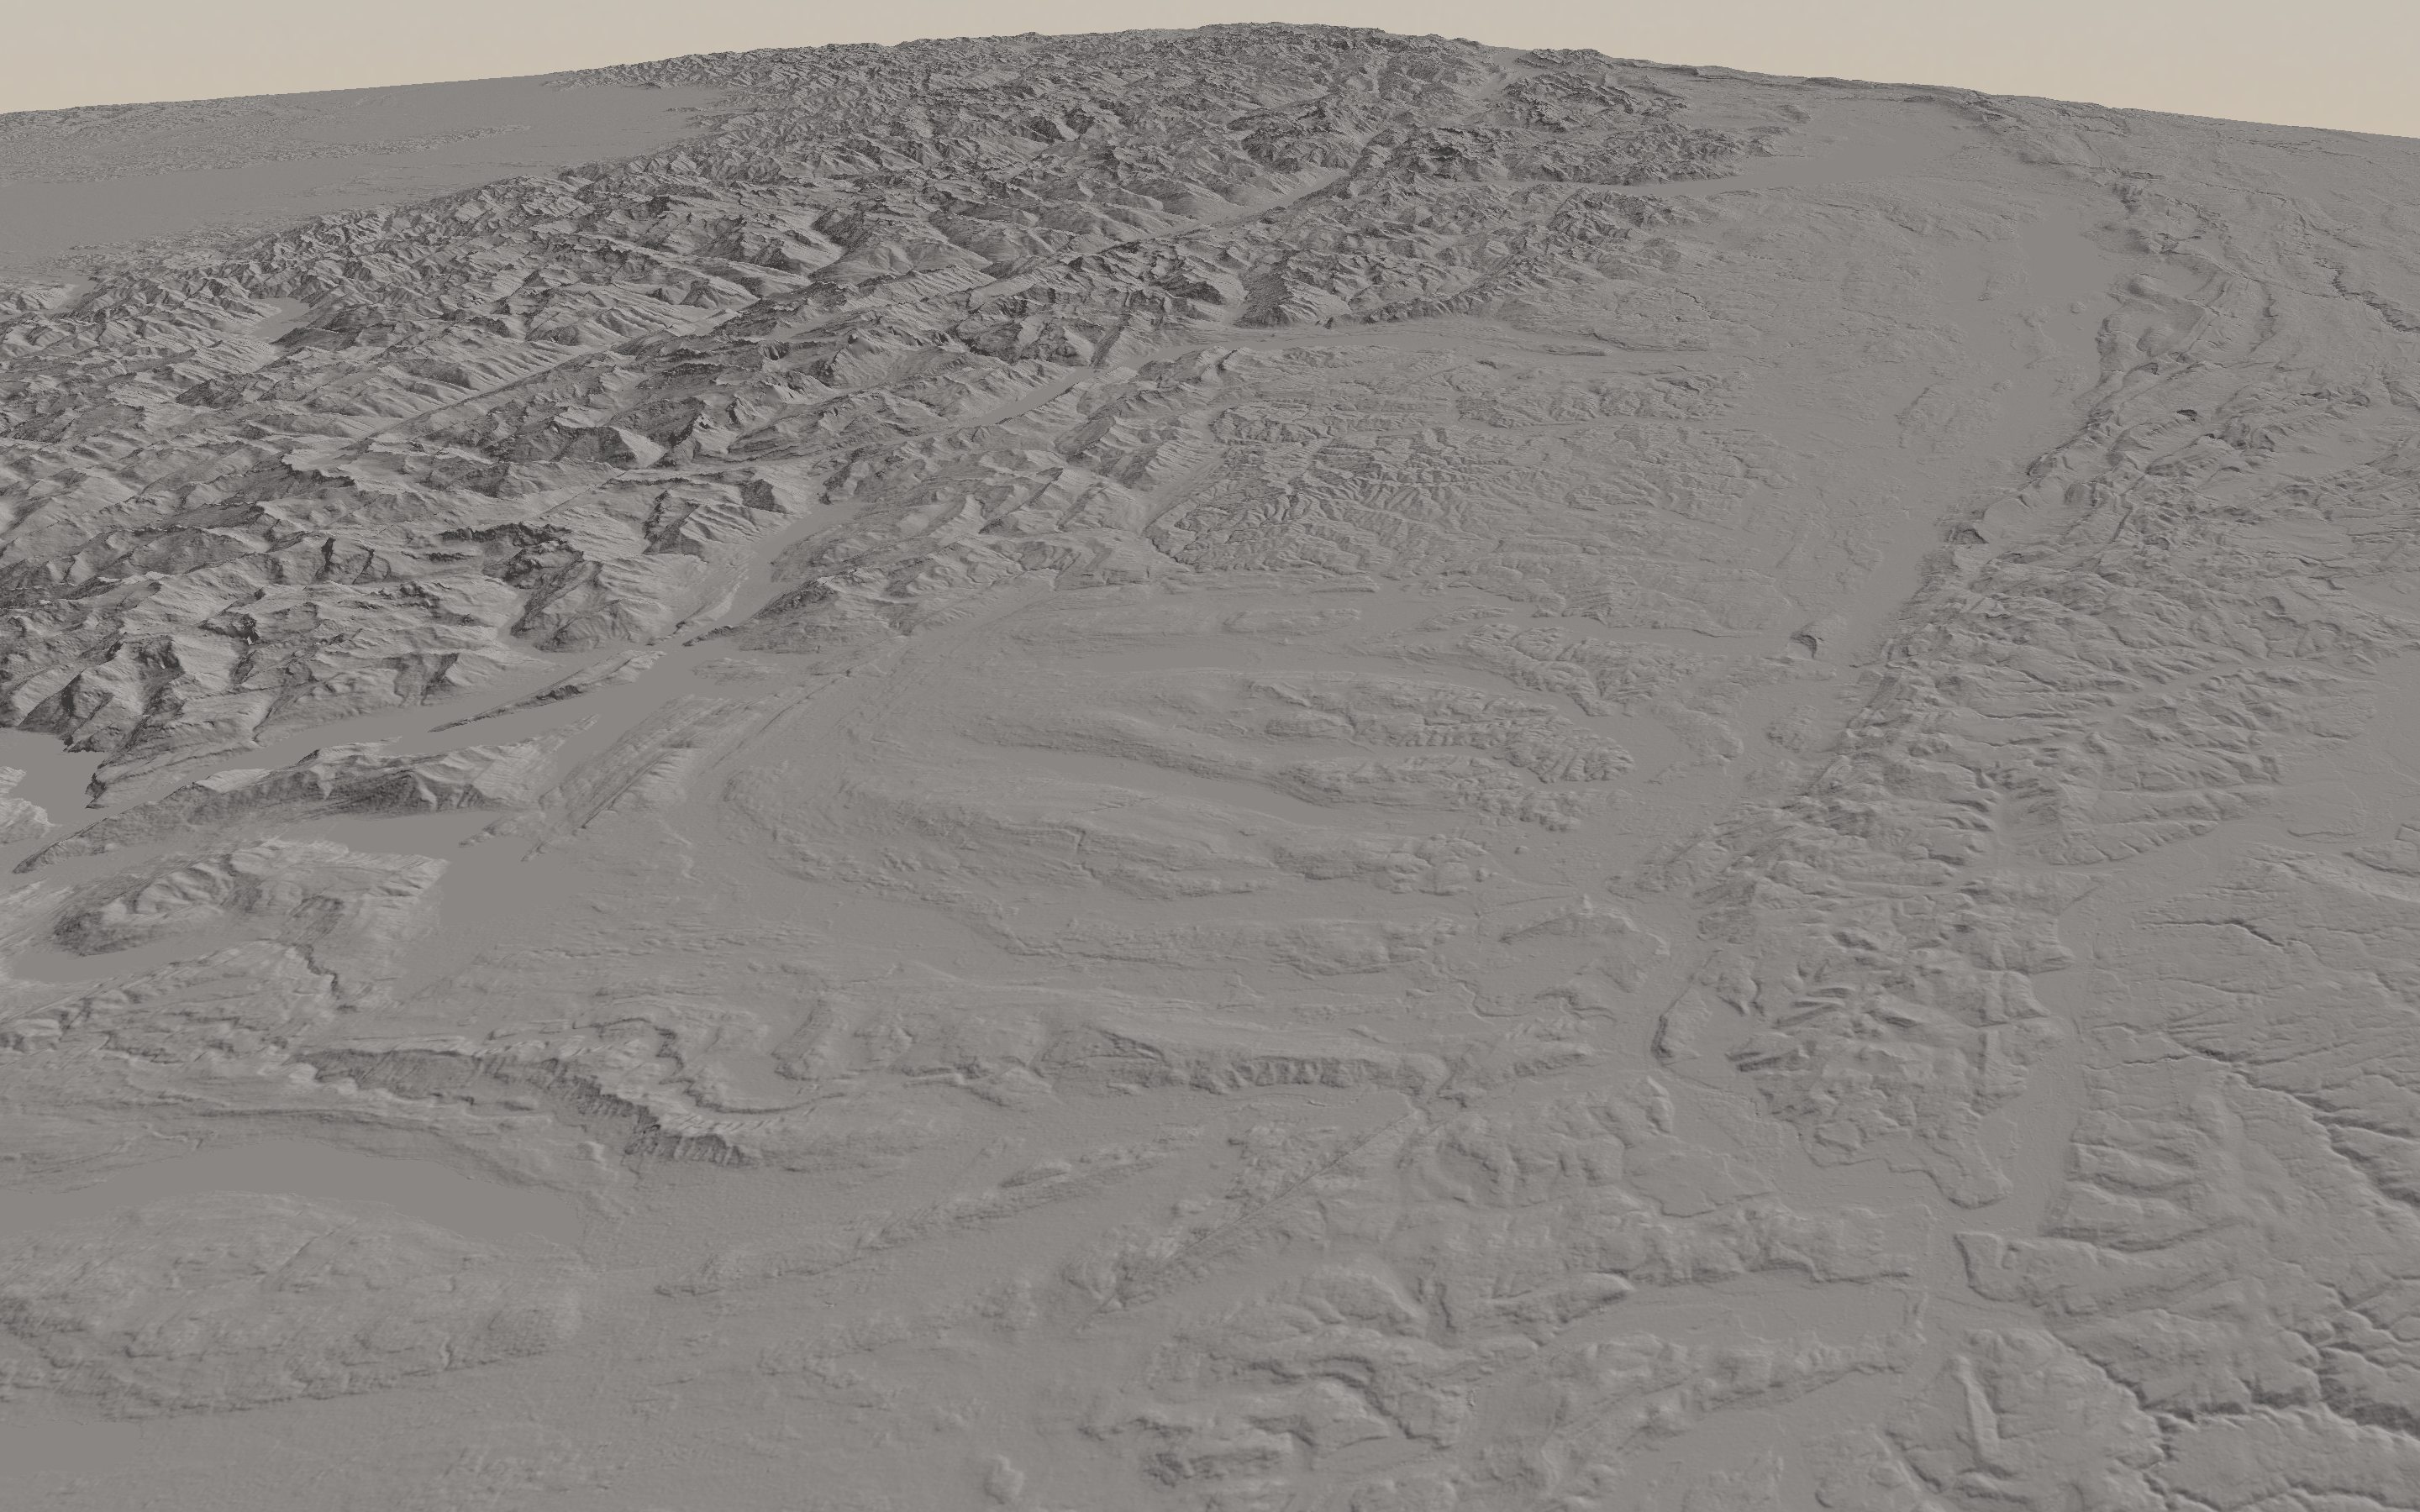
\includegraphics[width=0.4\textwidth]{results-accuracy-large-4-lod} }}
  \qquad
  \subfloat[\centering Absolute difference.]{{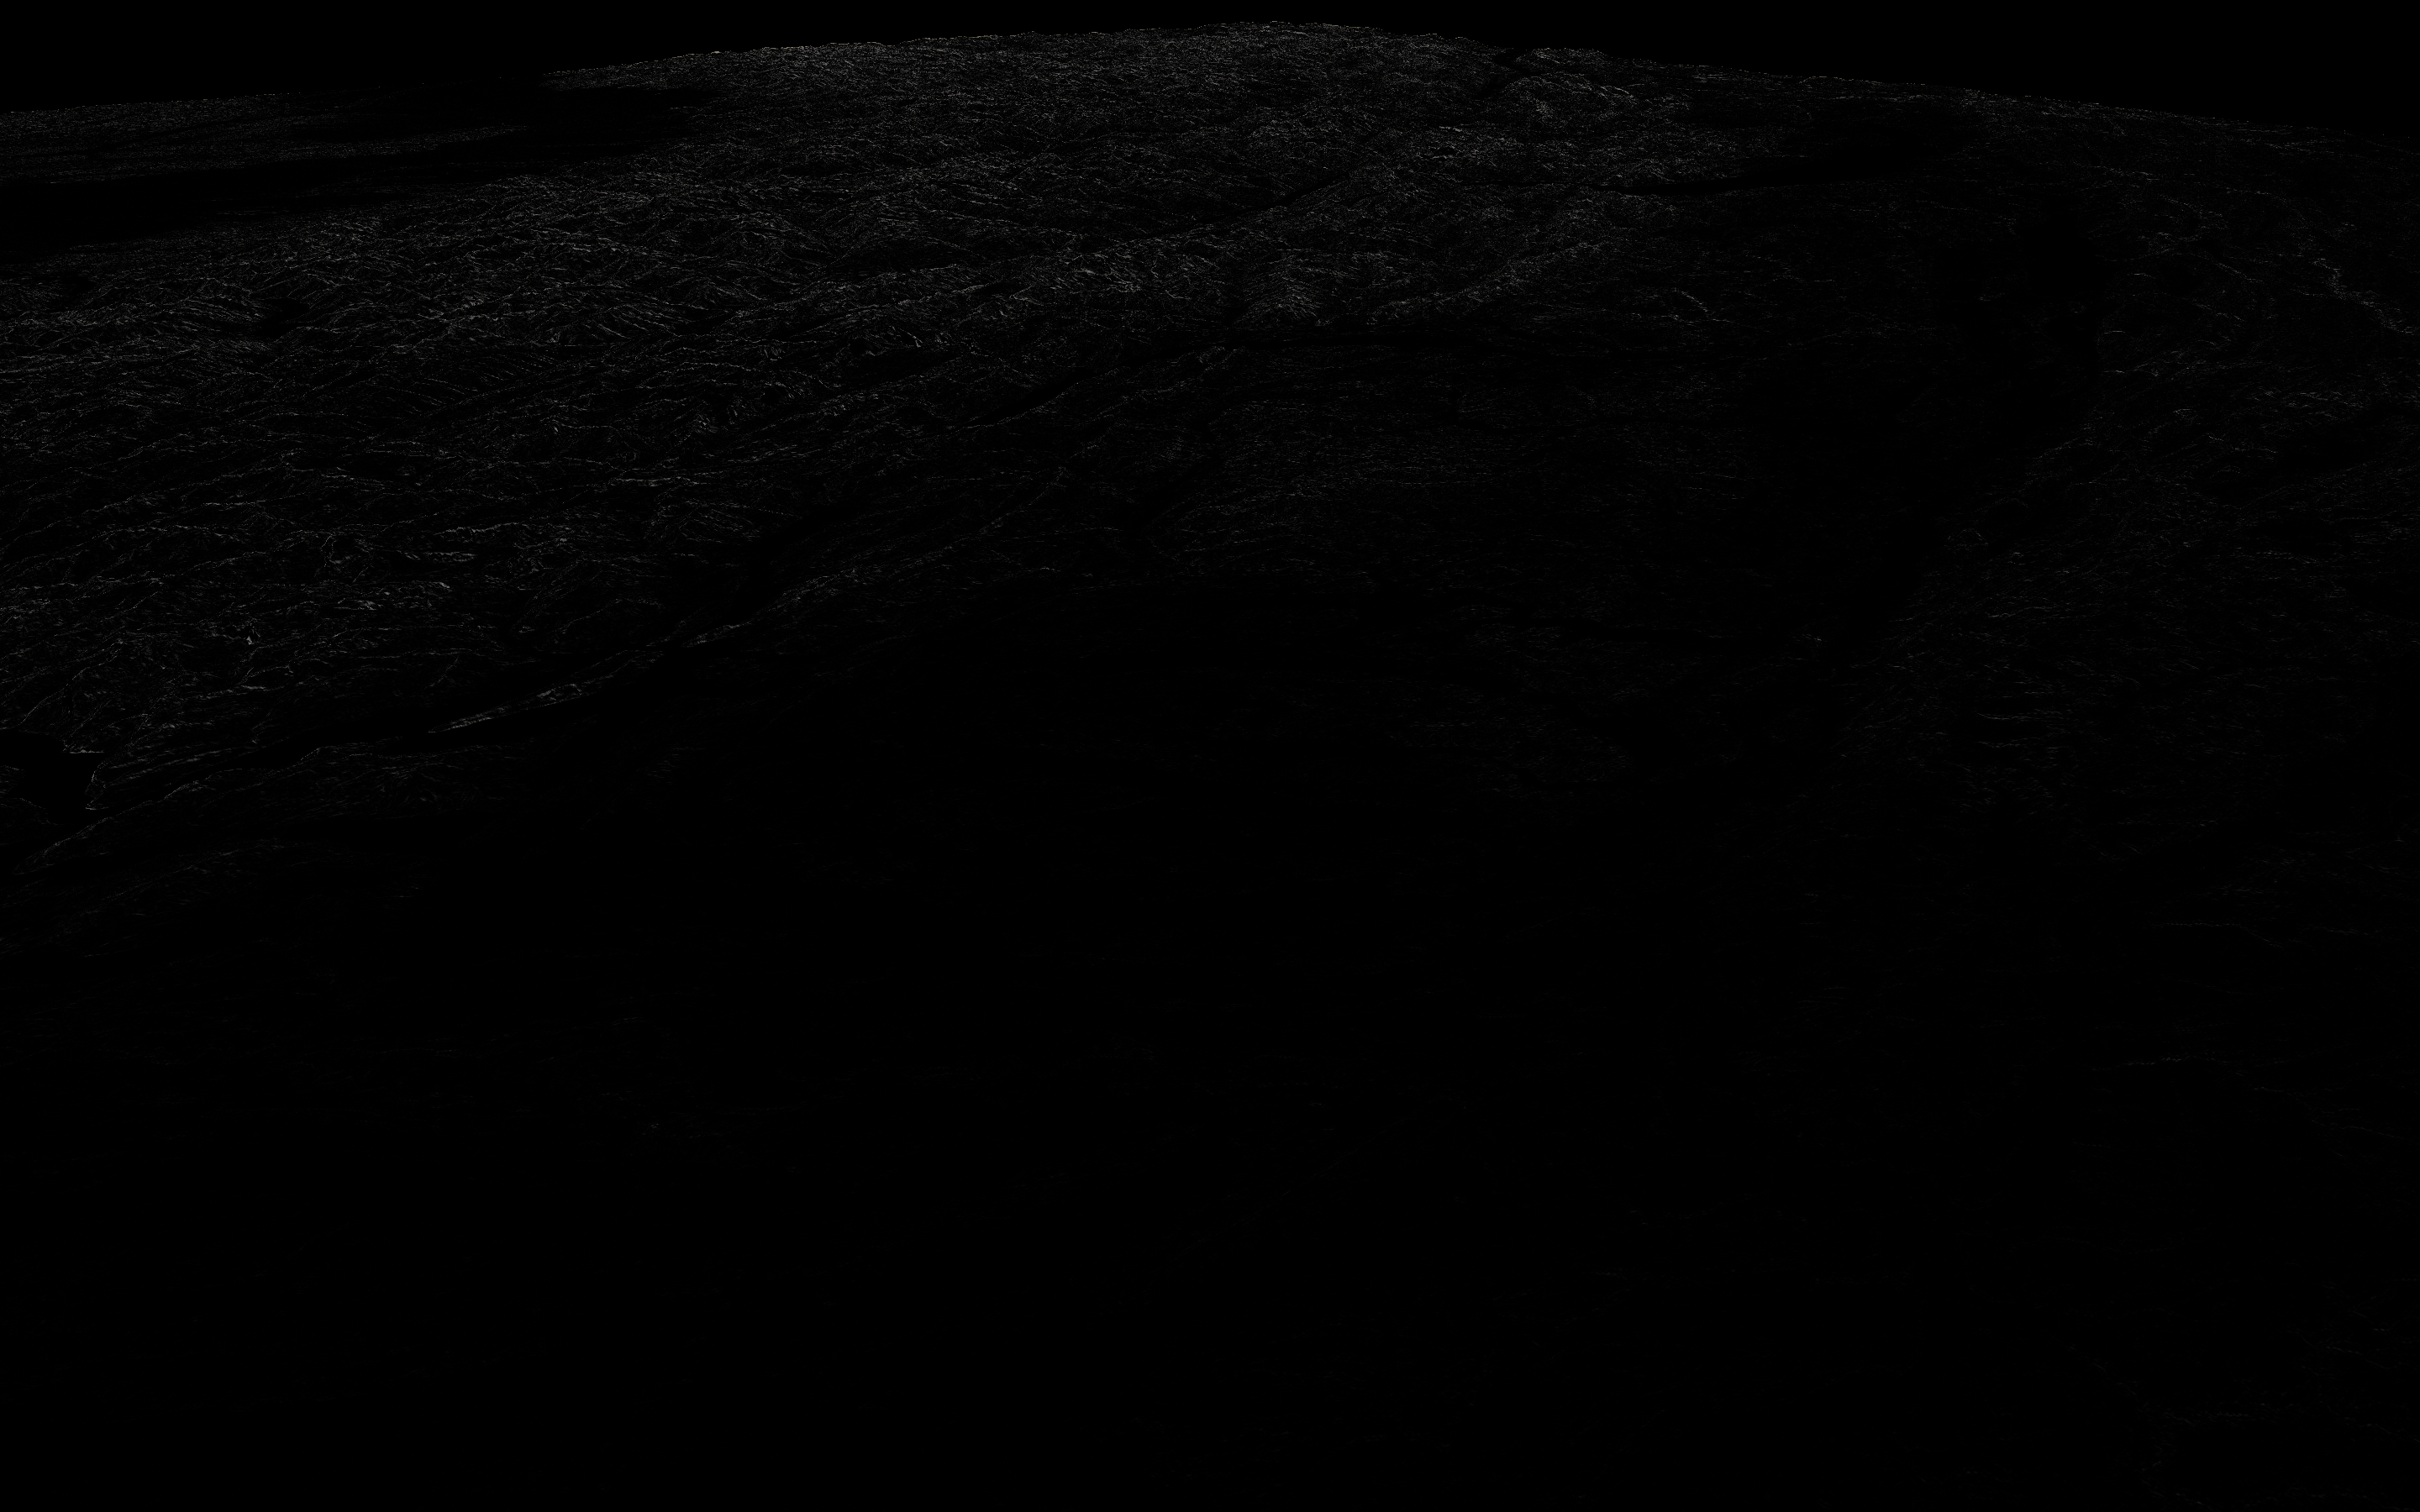
\includegraphics[width=0.4\textwidth]{results-accuracy-large-4-diff} }}
  \qquad
  \subfloat[\centering Absolute difference (binarised).]{{\includegraphics[width=0.4\textwidth]{results-accuracy-large-4-diff-bin} }}
  \caption{Screenshot showcasing the screenshot of a large section of the terrain with no LOD (a), with LOD (b),
   the absolute difference (c) between (a) and (b), and the binarised absolute difference (d) of (c). The computed RMSE is 1.96.}\label{fig:results-large-4}
\end{figure}
\subsubsection{Large Terrain Screenshot 5}
\begin{figure}[H]
  \centering
  \subfloat[\centering No LOD.]{{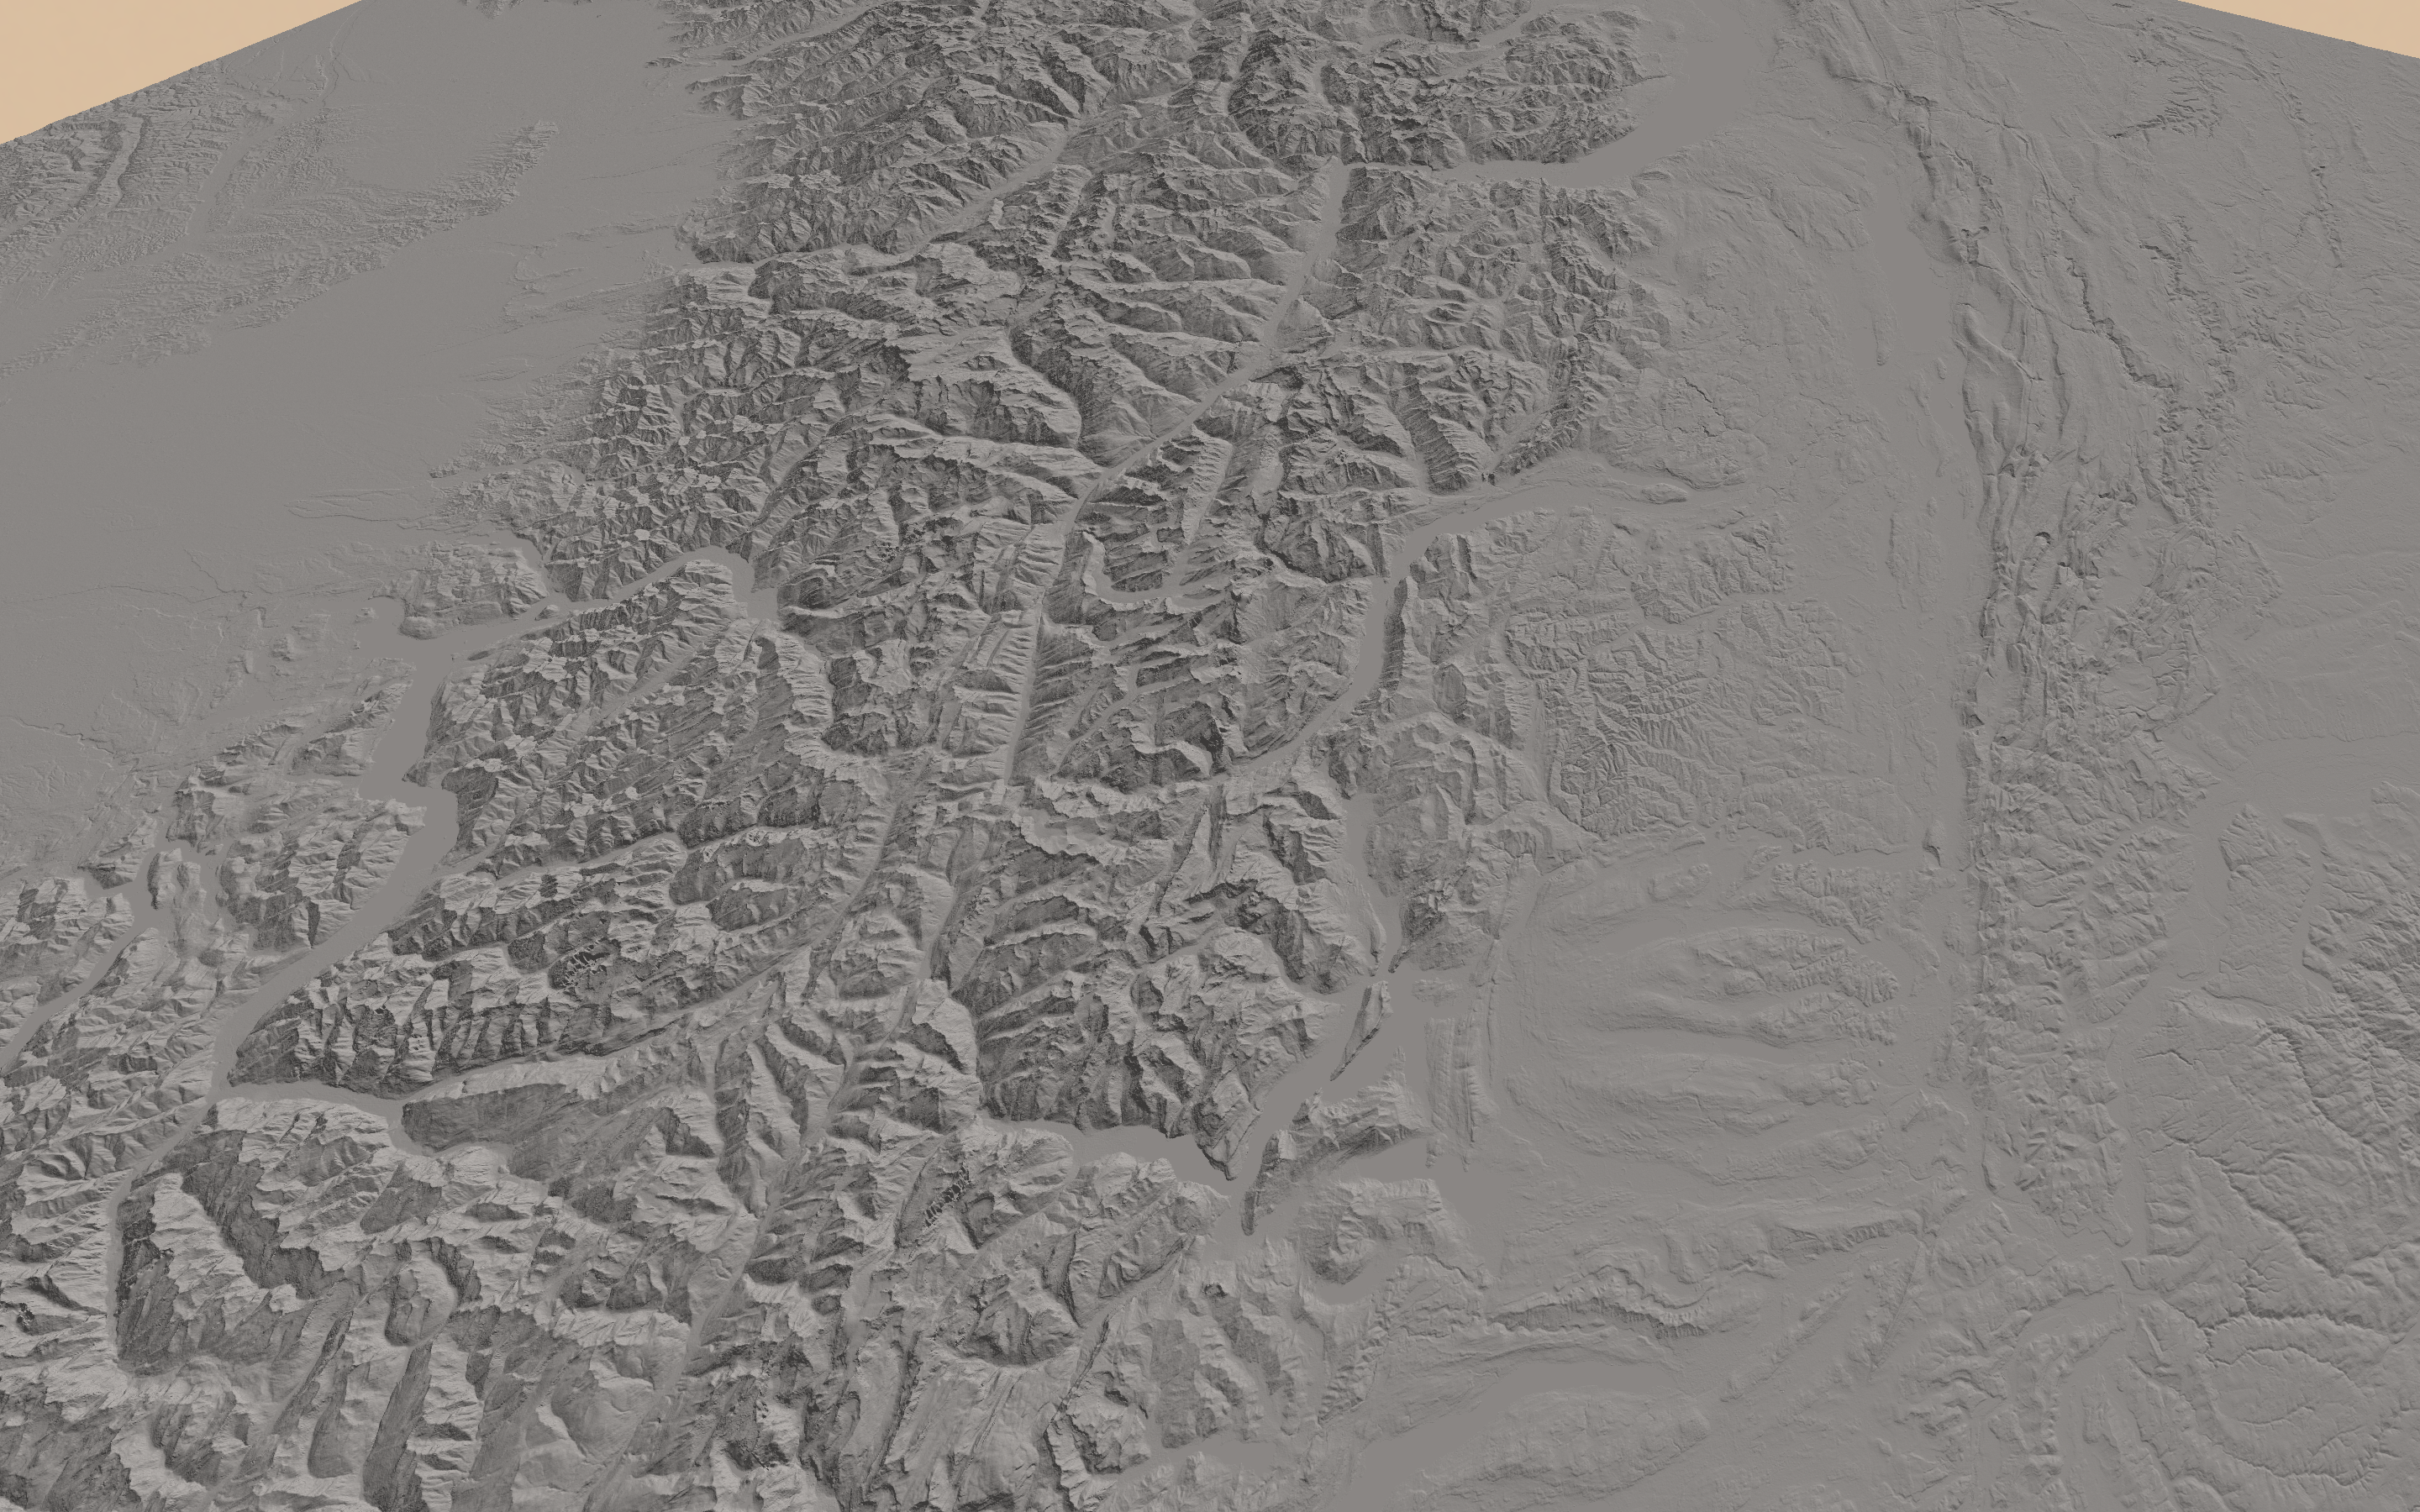
\includegraphics[width=0.4\textwidth]{results-accuracy-large-5-no-lod} }}
  \qquad
  \subfloat[\centering With LOD.]{{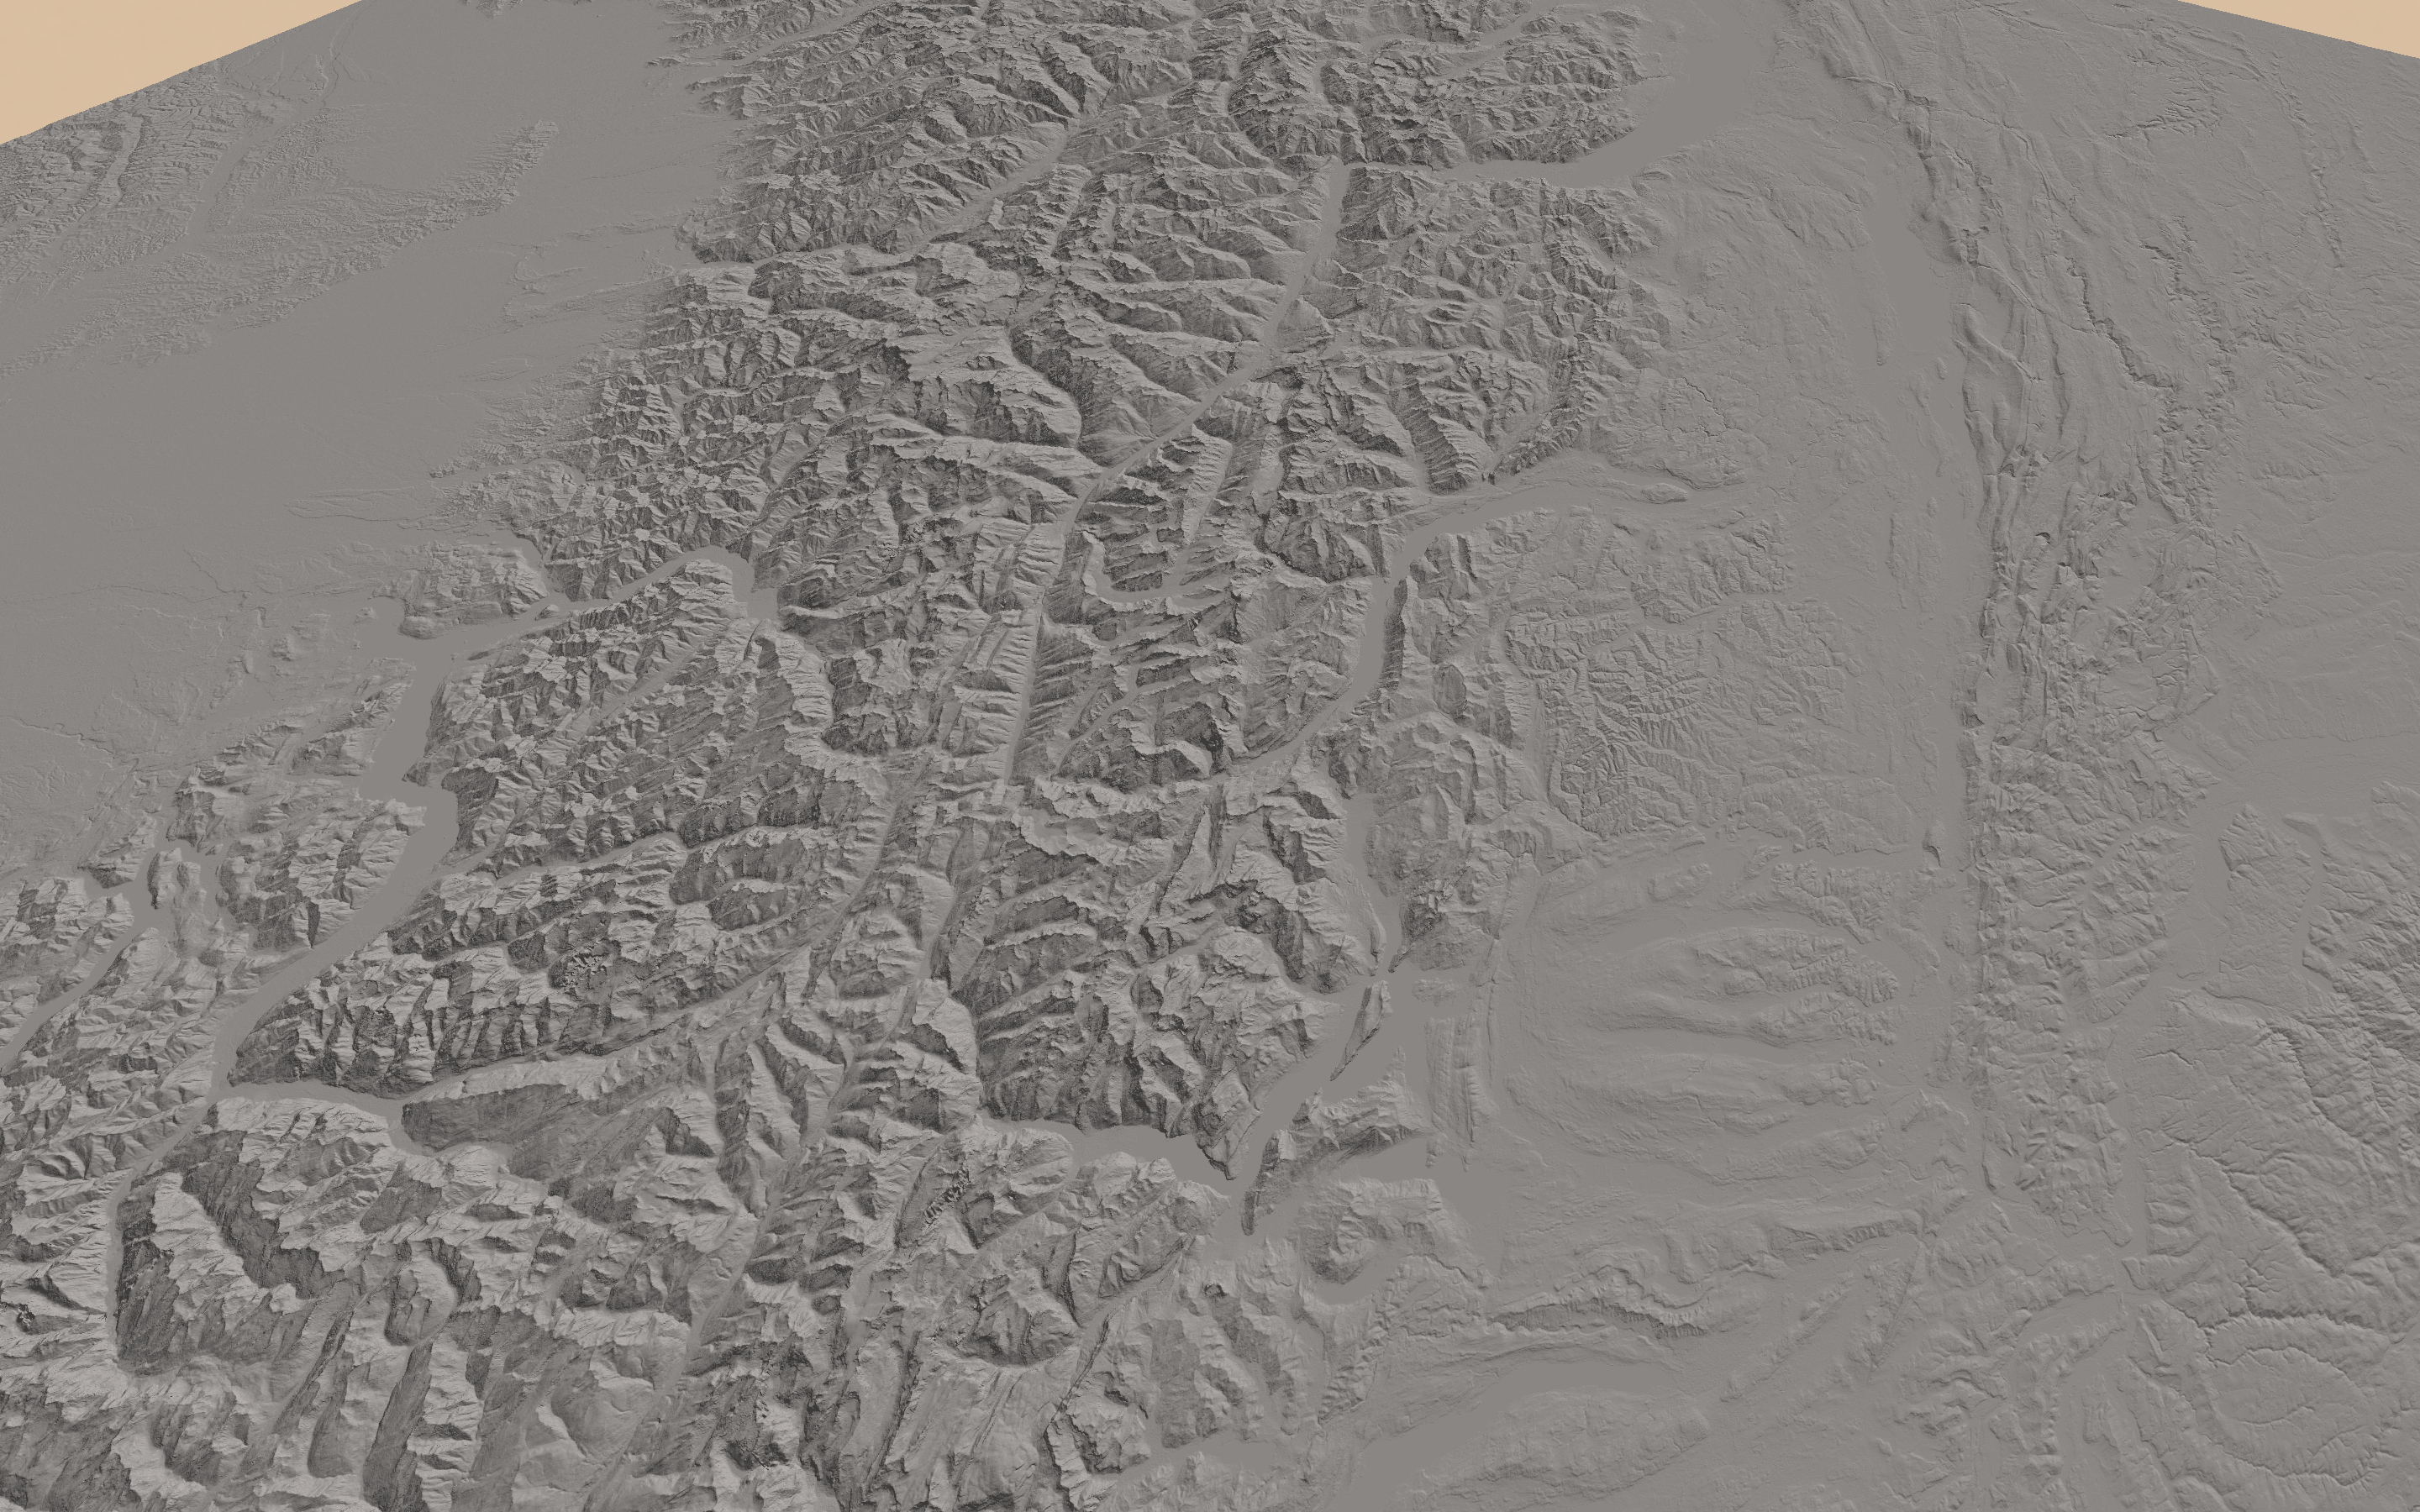
\includegraphics[width=0.4\textwidth]{results-accuracy-large-5-lod} }}
  \qquad
  \subfloat[\centering Absolute difference.]{{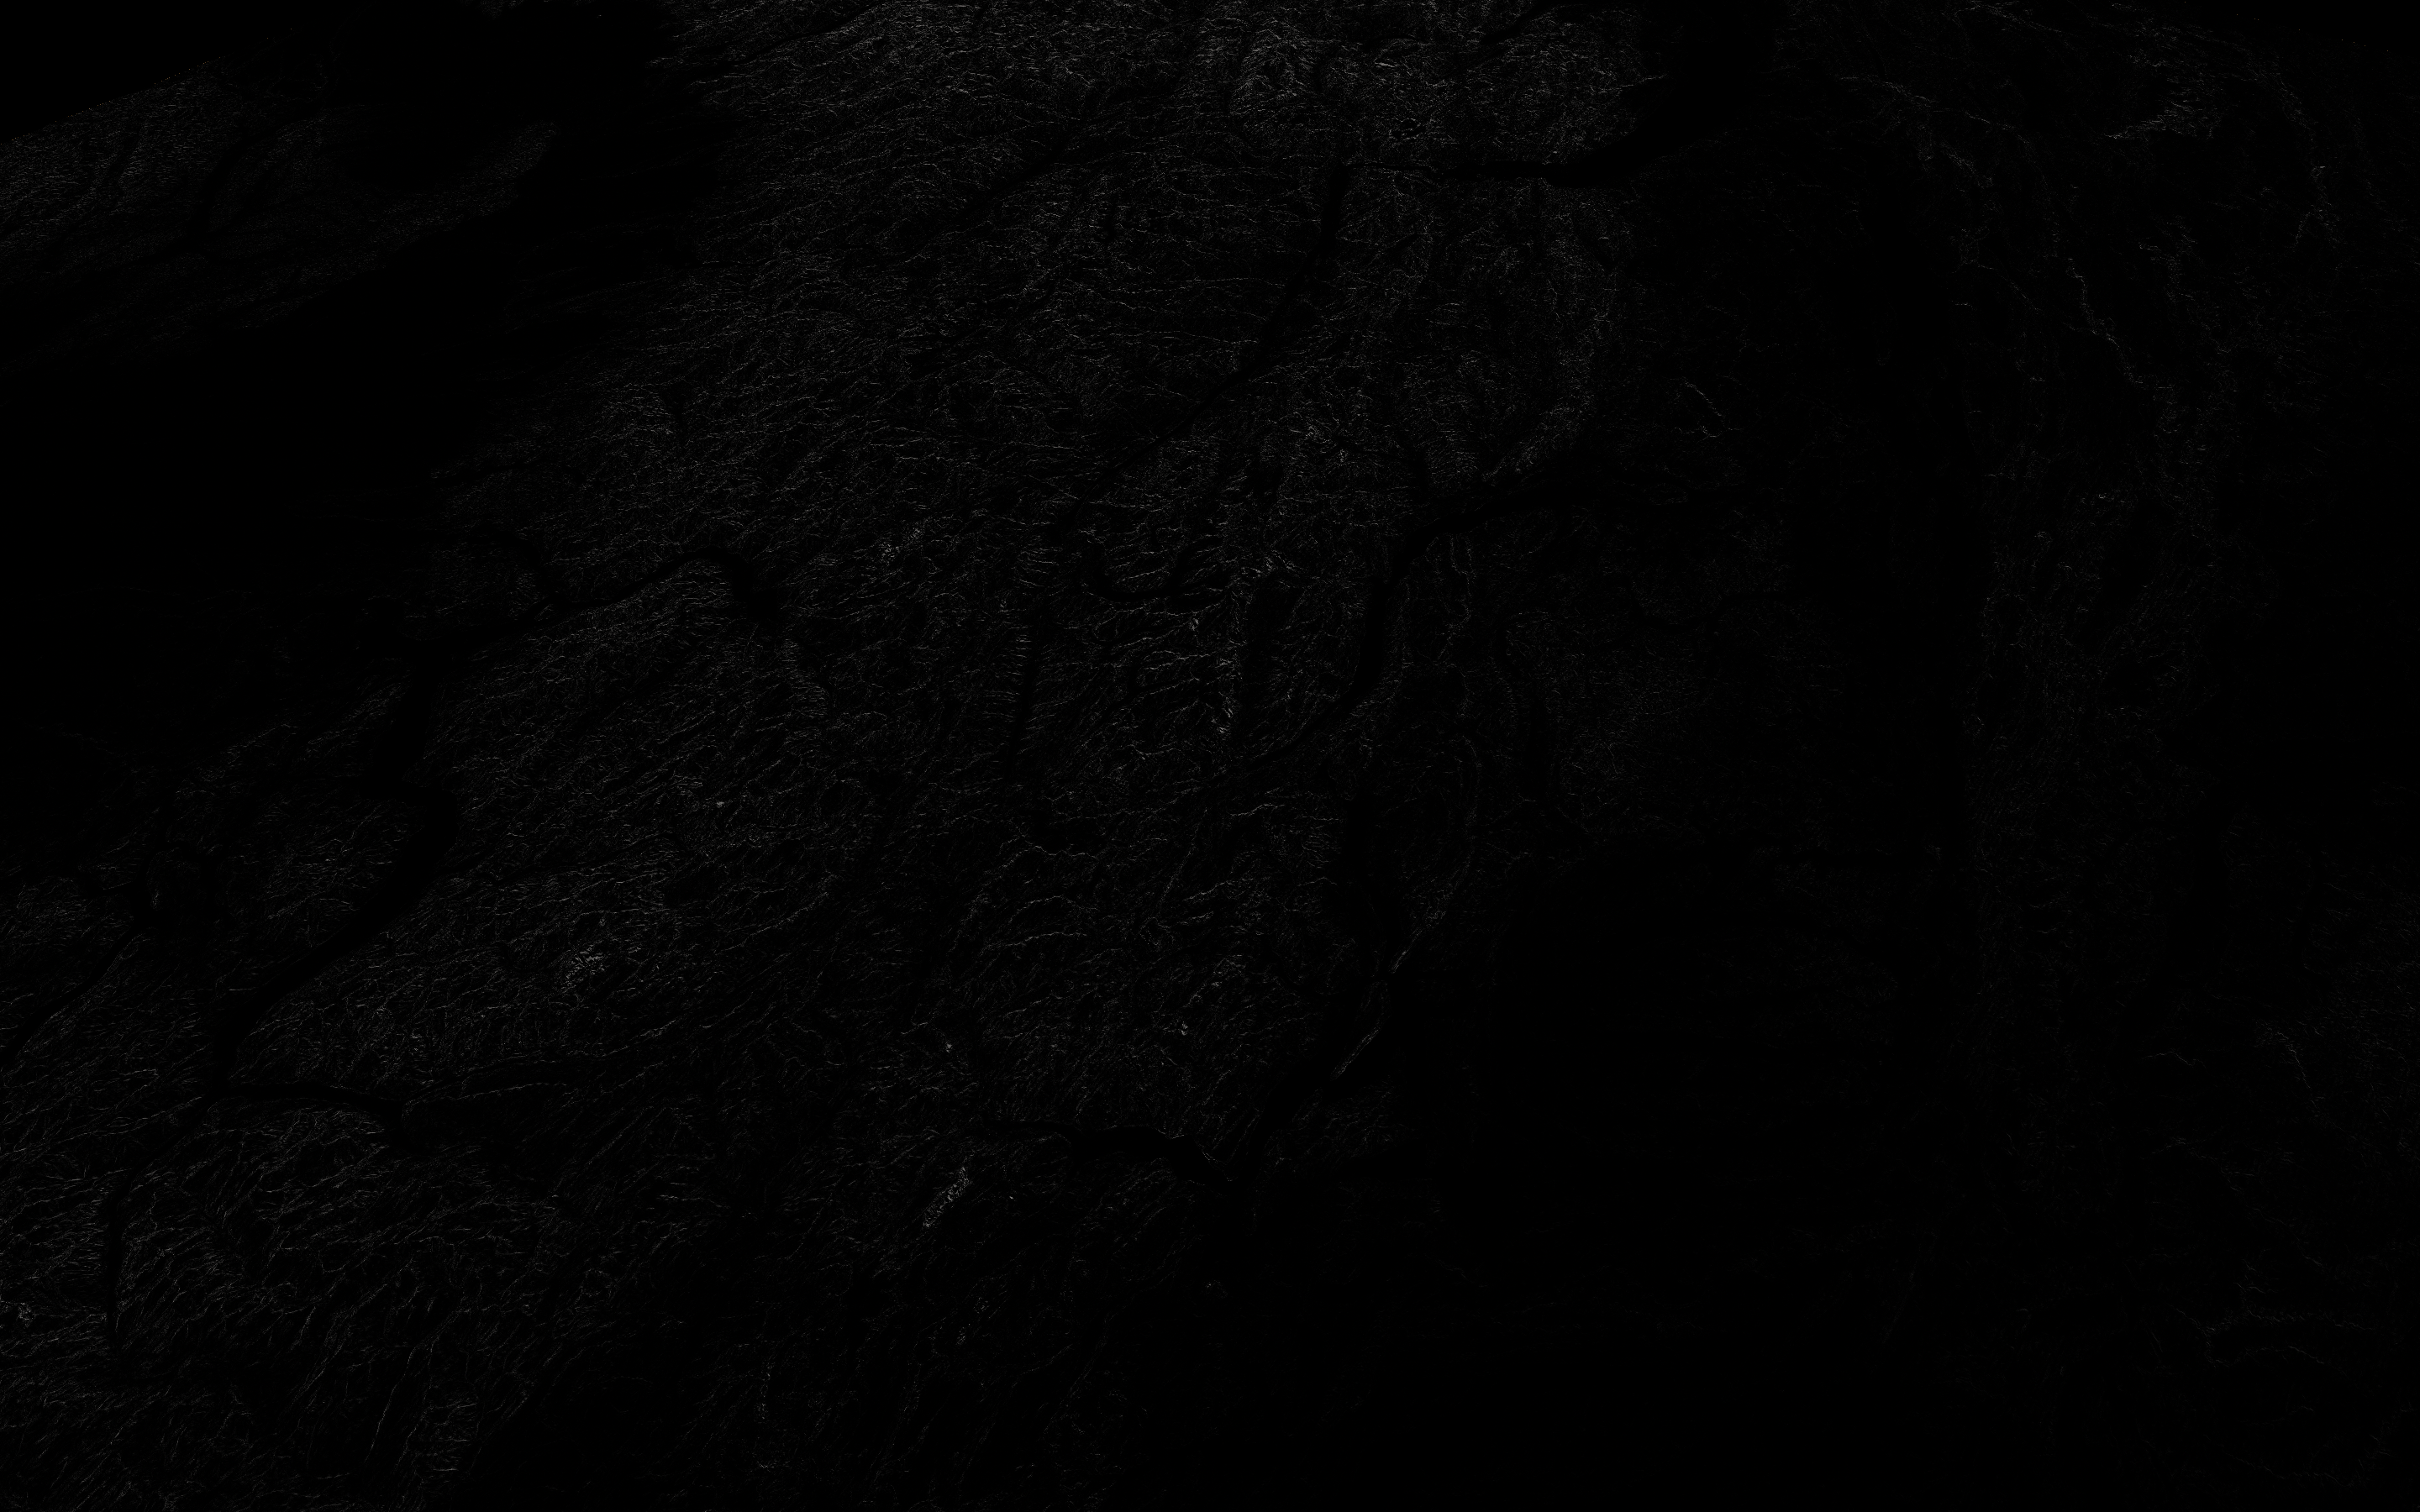
\includegraphics[width=0.4\textwidth]{results-accuracy-large-5-diff} }}
  \qquad
  \subfloat[\centering Absolute difference (binarised).]{{\includegraphics[width=0.4\textwidth]{results-accuracy-large-5-diff-bin} }}
  \caption{Screenshot showcasing the screenshot of a large section of the terrain with no LOD (a), with LOD (b),
   the absolute difference (c) between (a) and (b), and the binarised absolute difference (d) of (c). The computed RMSE is 2.32.}\label{fig:results-large-5}
\end{figure}

\subsubsection{Low FOV Screenshot 1}
\begin{figure}[H]
  \centering
  \subfloat[\centering No LOD.]{{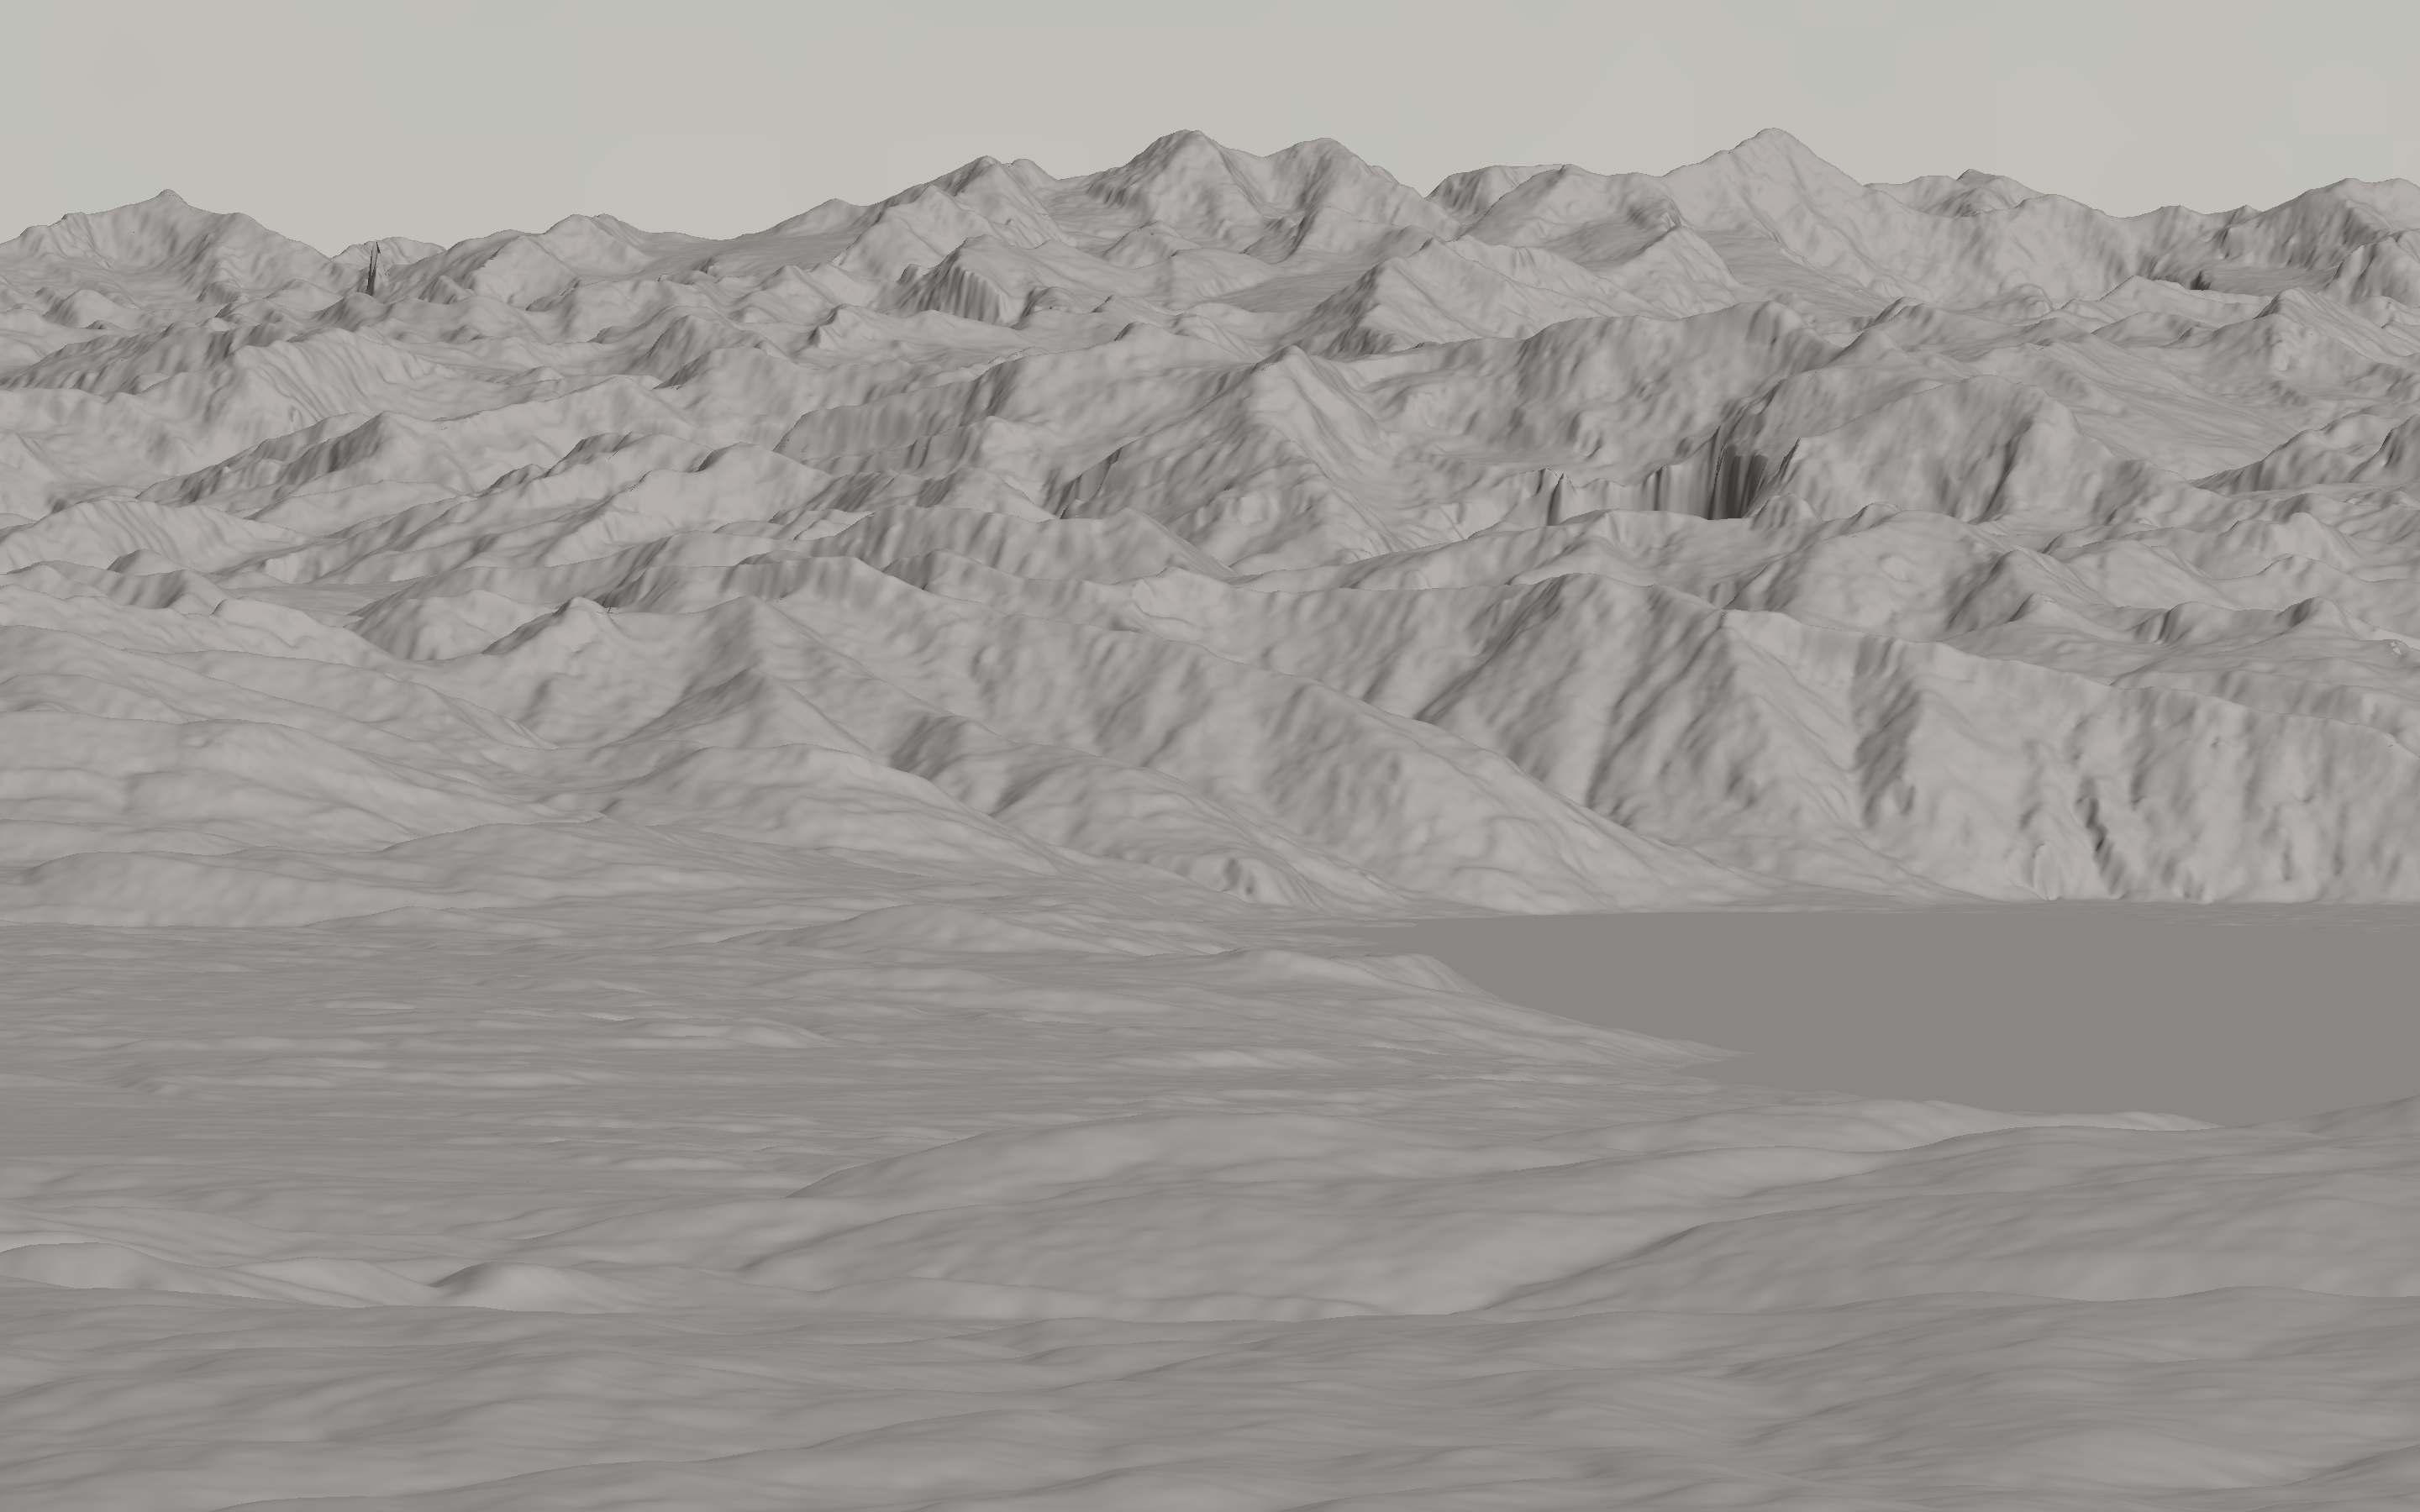
\includegraphics[width=0.4\textwidth]{results-accuracy-zoom-1-no-lod} }}
  \qquad
  \subfloat[\centering With LOD.]{{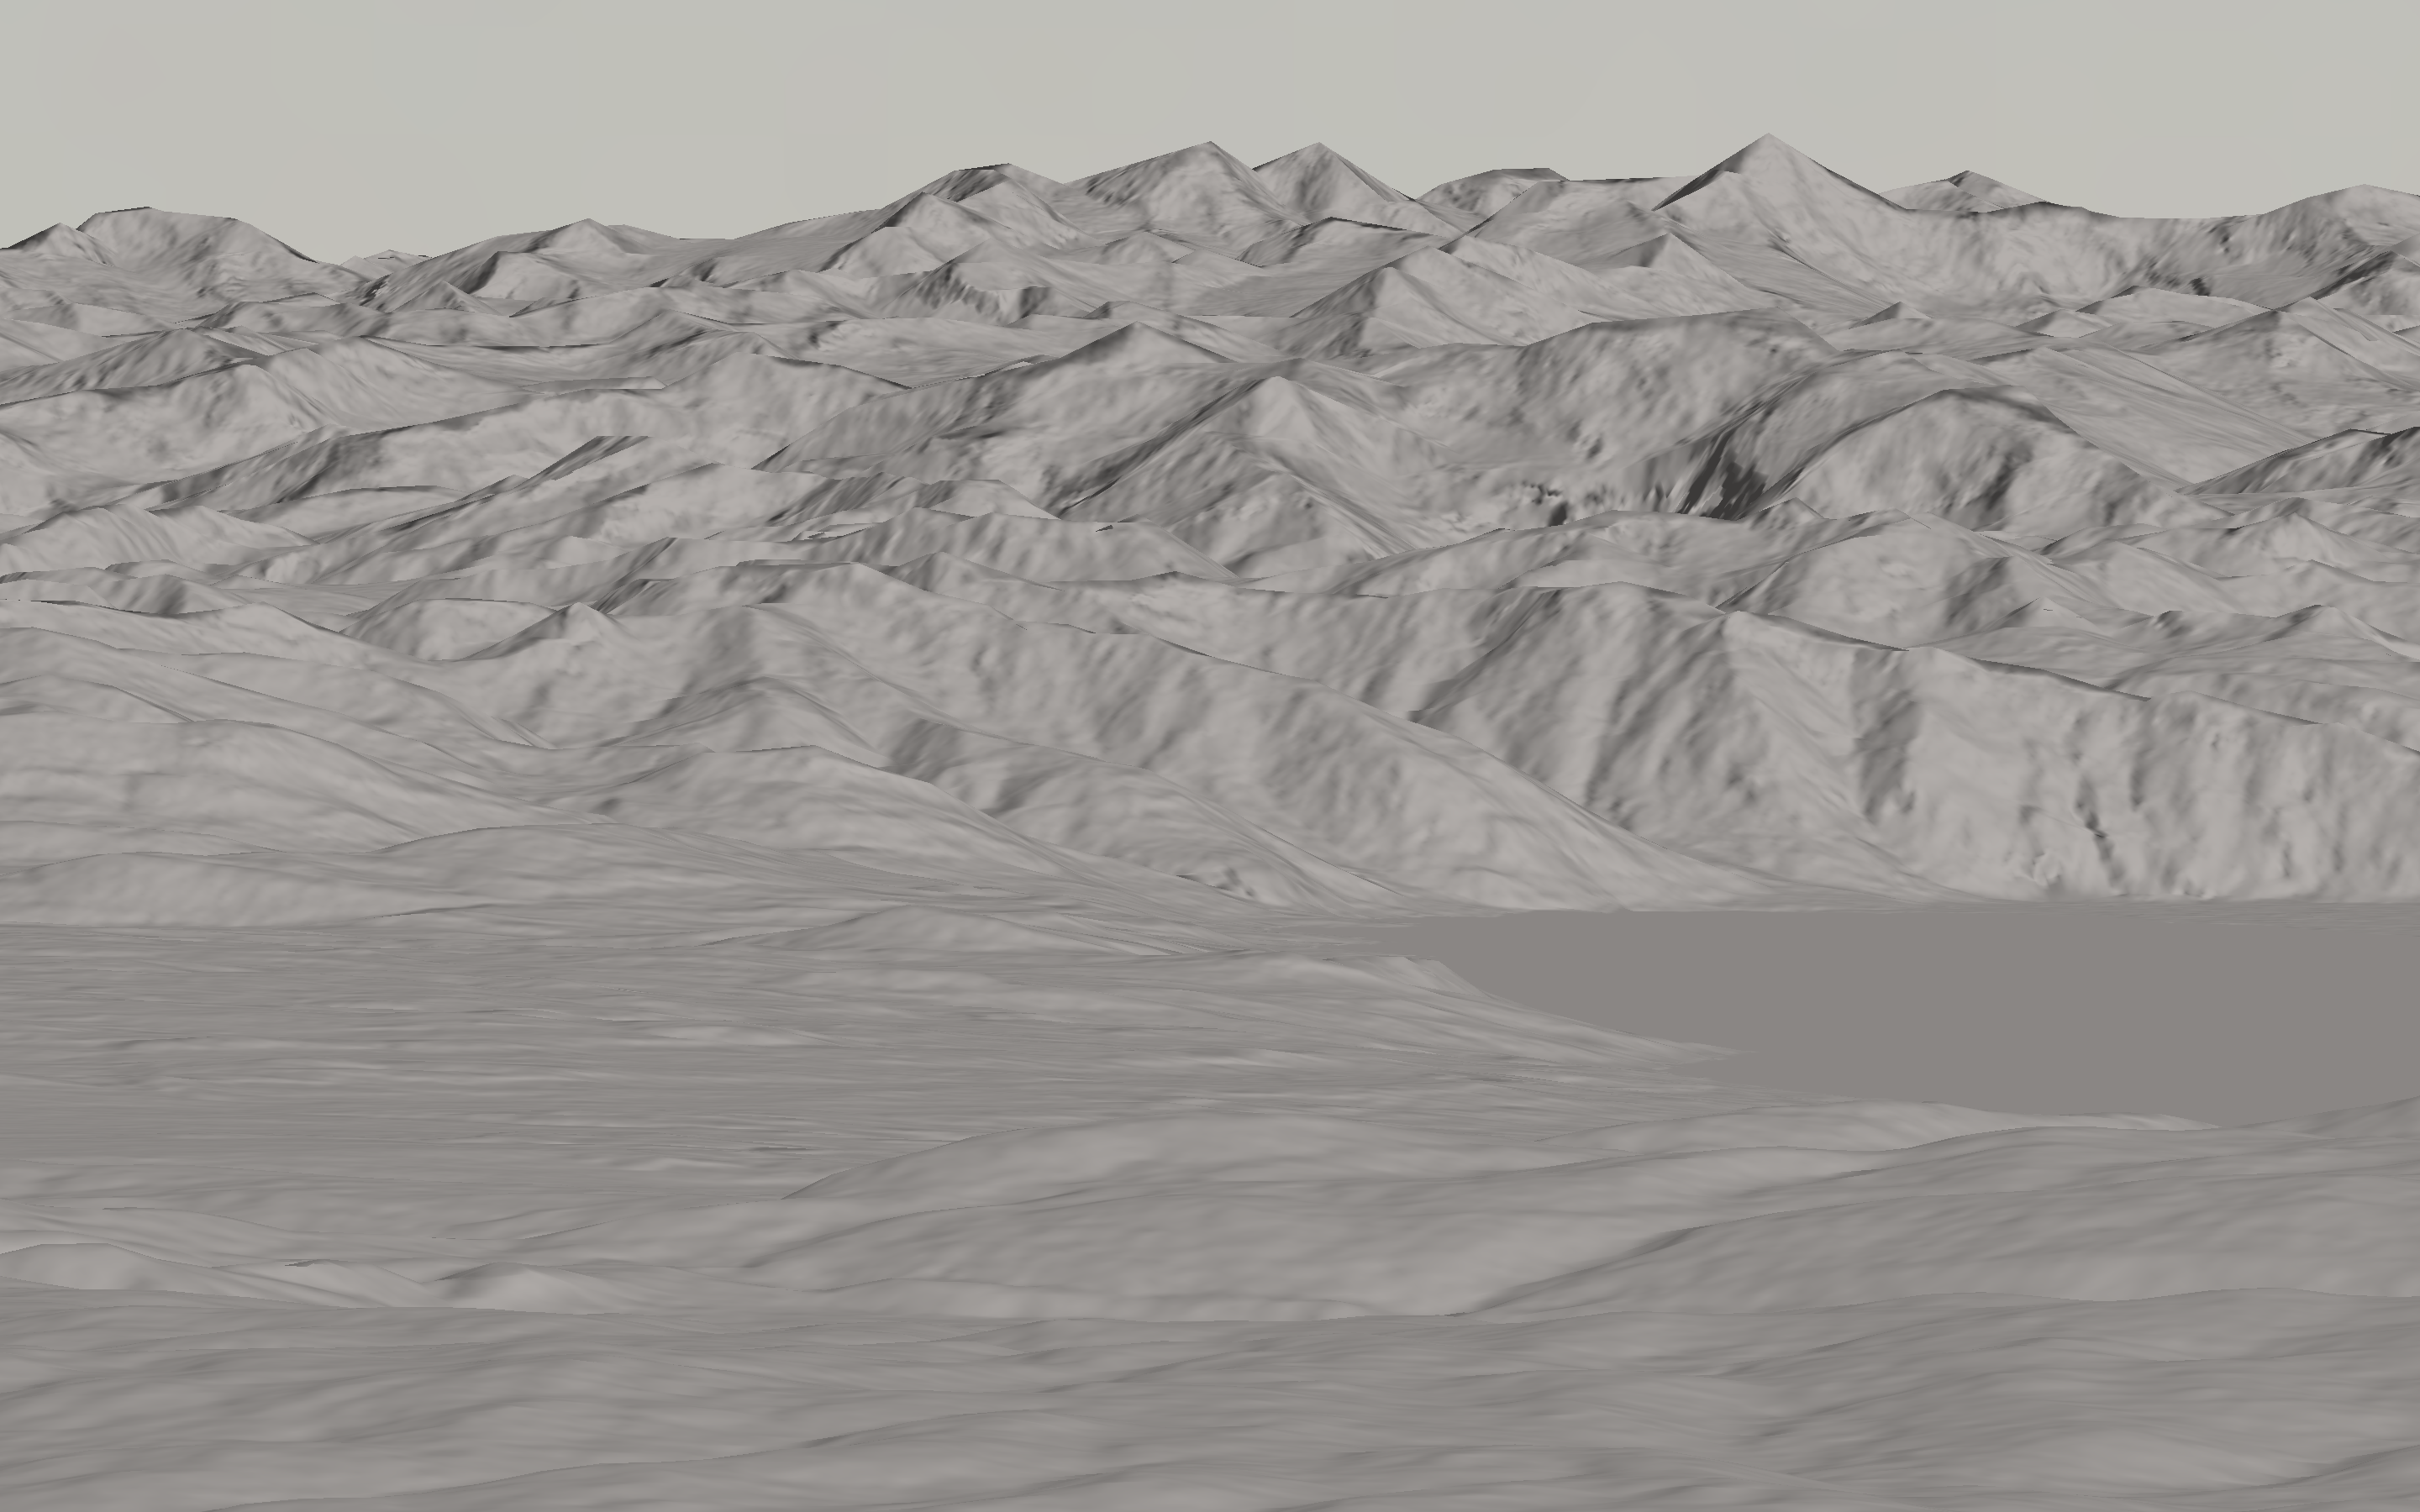
\includegraphics[width=0.4\textwidth]{results-accuracy-zoom-1-lod} }}
  \qquad
  \subfloat[\centering Absolute difference.]{{\includegraphics[width=0.4\textwidth]{results-accuracy-zoom-1-diff} }}
  \qquad
  \subfloat[\centering Absolute difference (binarised).]{{\includegraphics[width=0.4\textwidth]{results-accuracy-zoom-1-diff-bin} }}
  \caption{Screenshot showcasing the screenshot of a small section of the terrain with no LOD (a), with LOD (b),
  the absolute difference (c) between (a) and (b) and the binarised absolute difference (d) of (c). The FOV is set to $6^{\circ}$ and the computed RSME is 4.82.}\label{fig:results-zoom-1}
\end{figure}
\subsubsection{Low FOV Screenshot 2}
\begin{figure}[H]
  \centering
  \subfloat[\centering No LOD.]{{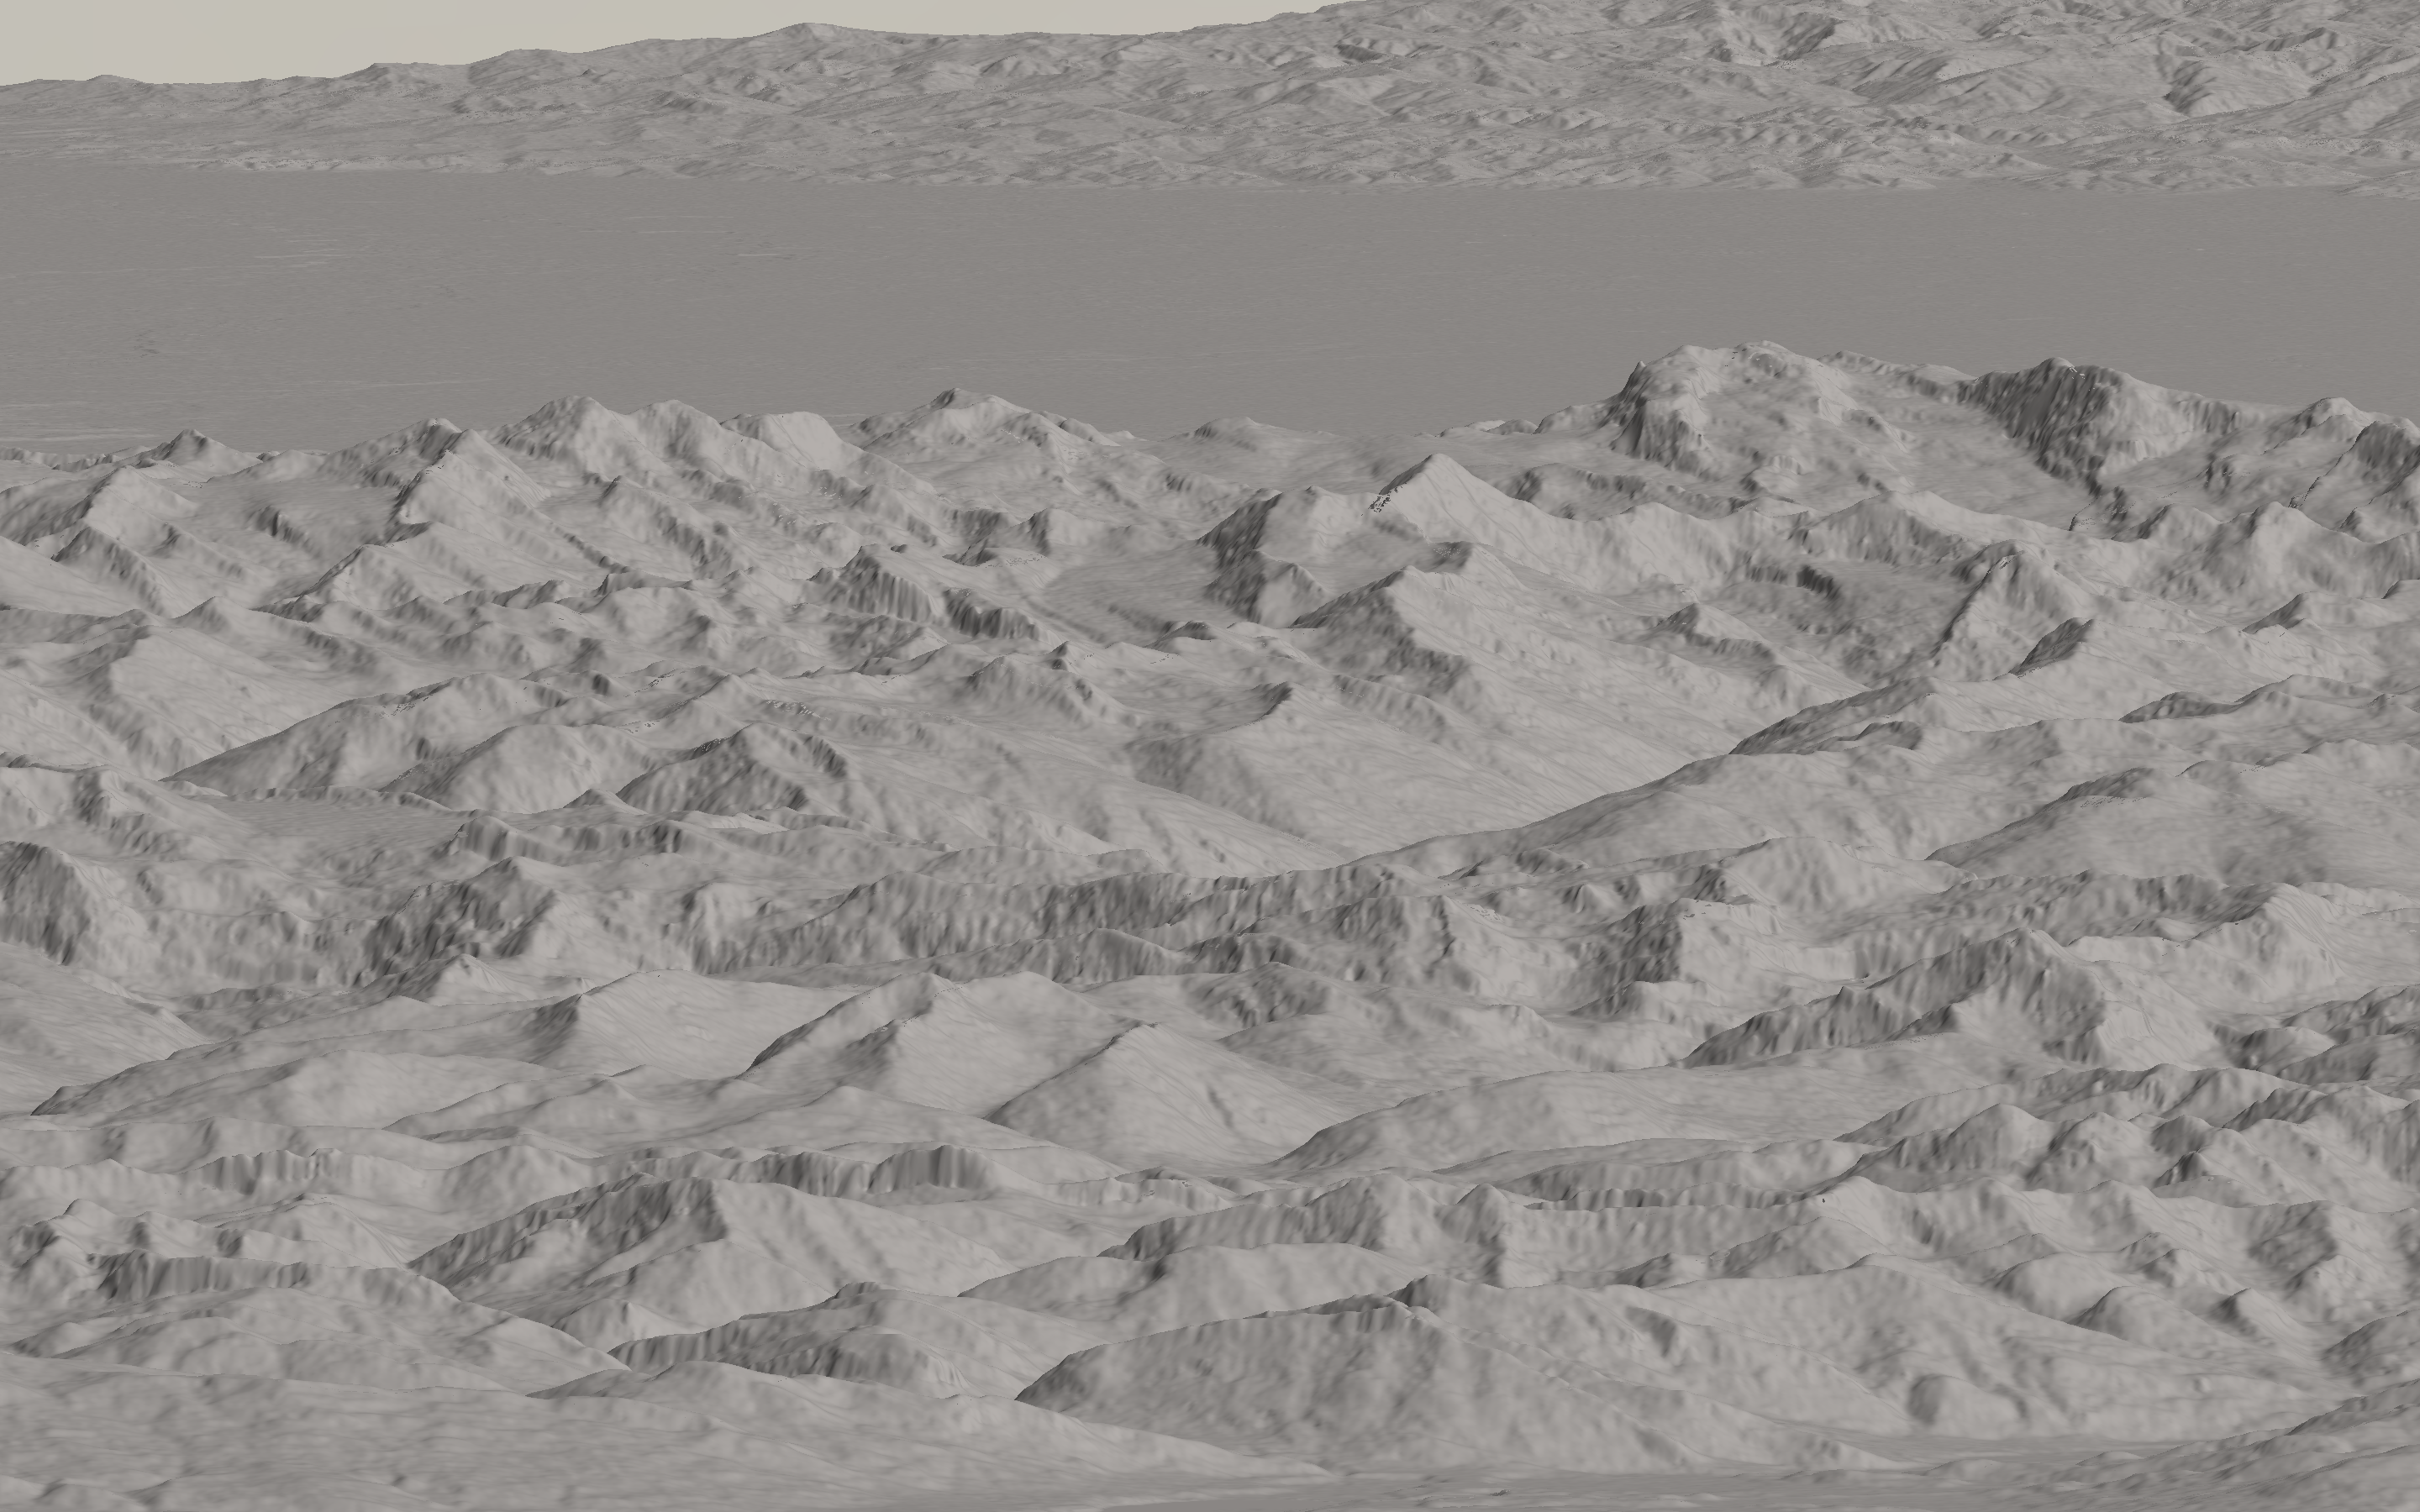
\includegraphics[width=0.4\textwidth]{results-accuracy-zoom-2-no-lod} }}
  \qquad
  \subfloat[\centering With LOD.]{{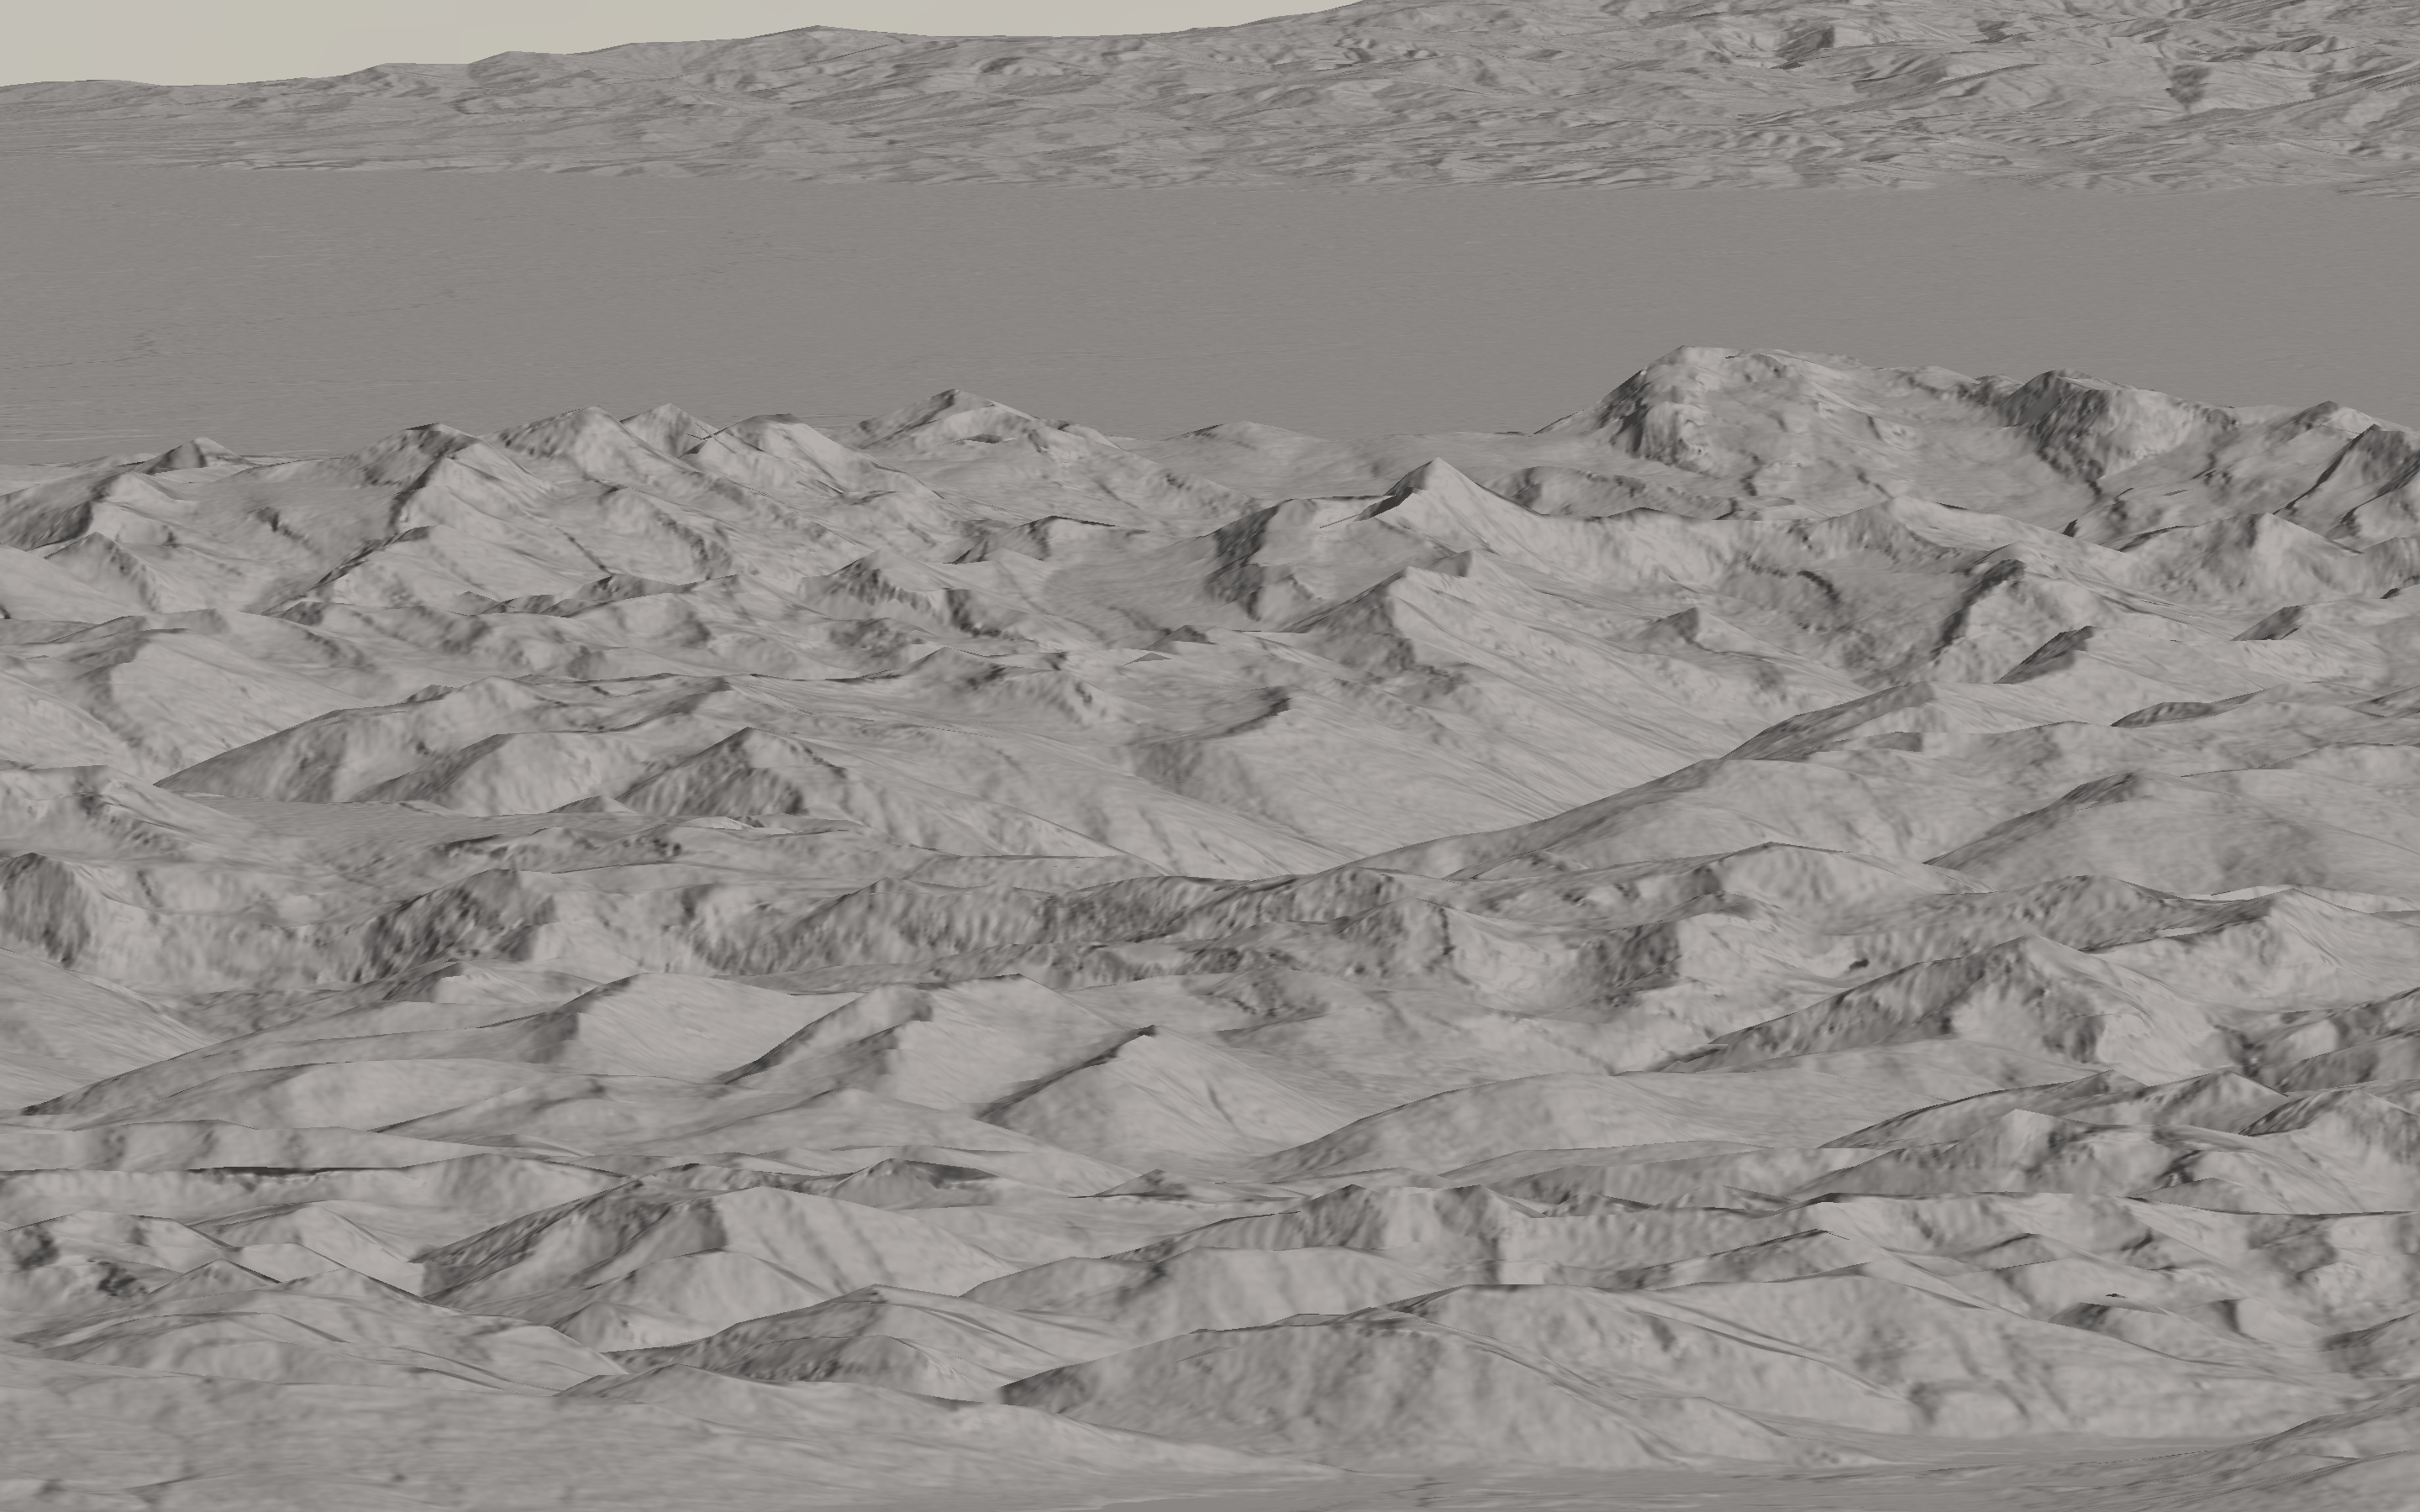
\includegraphics[width=0.4\textwidth]{results-accuracy-zoom-2-lod} }}
  \qquad
  \subfloat[\centering Absolute difference.]{{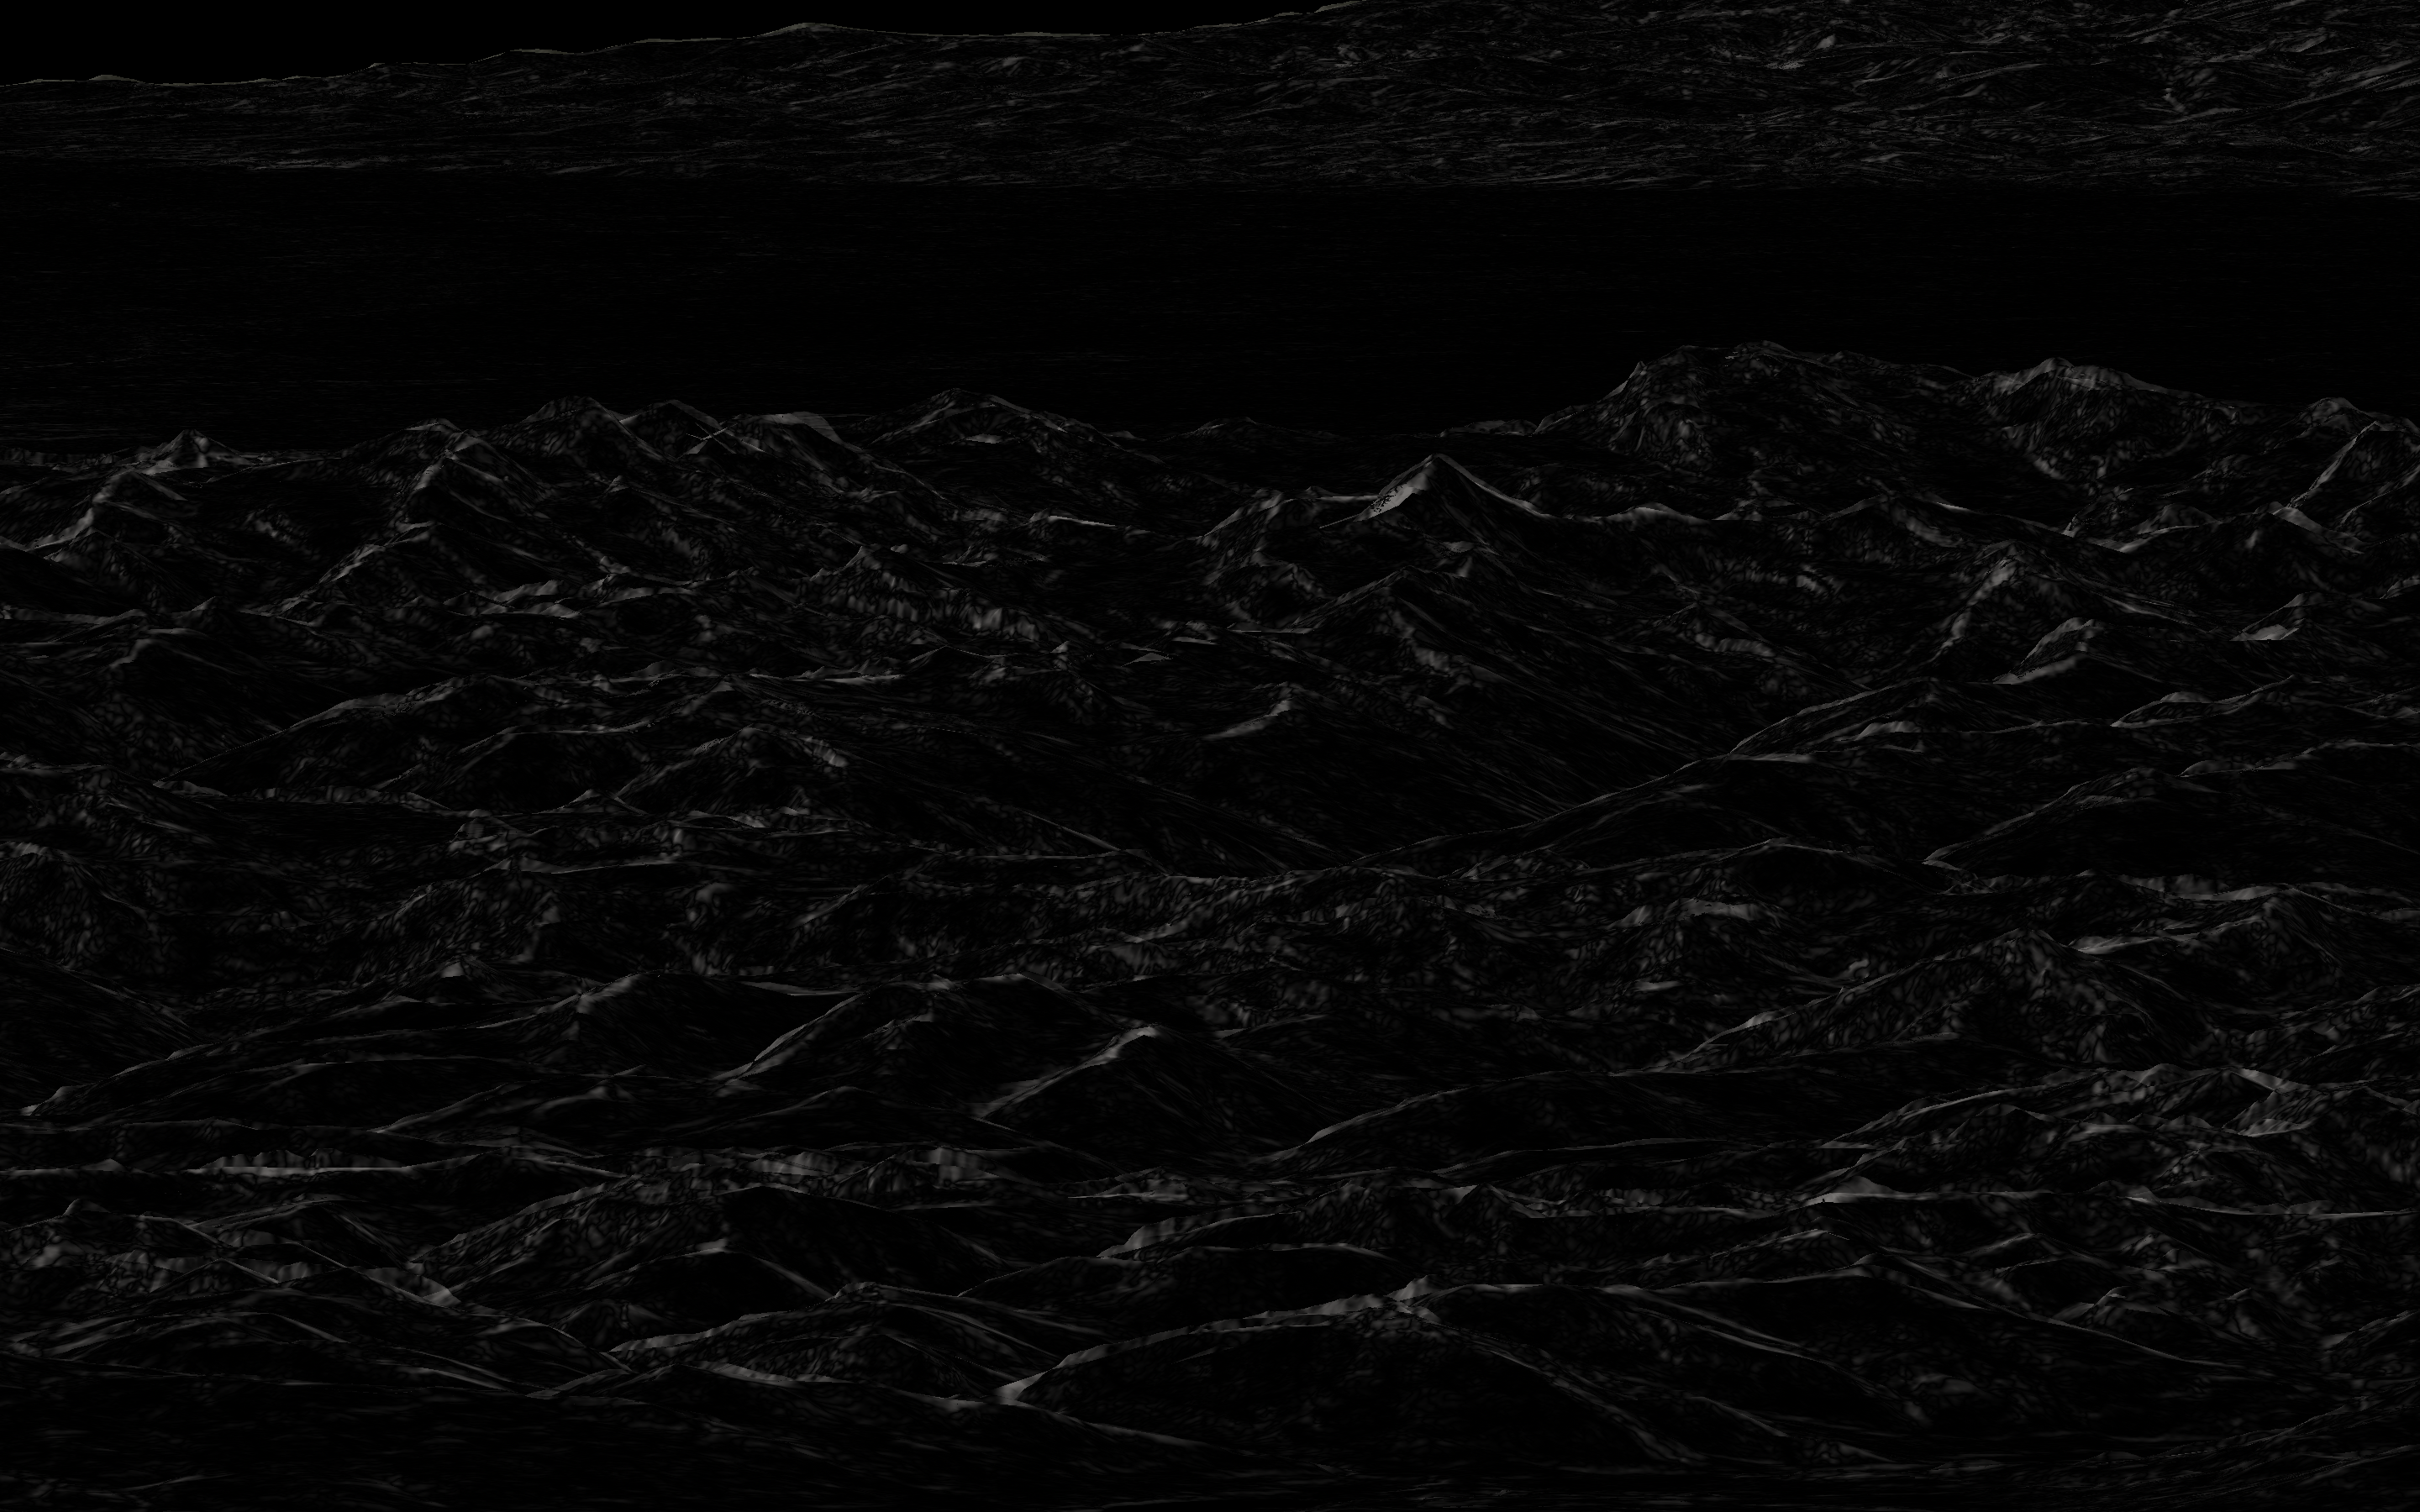
\includegraphics[width=0.4\textwidth]{results-accuracy-zoom-2-diff} }}
  \qquad
  \subfloat[\centering Absolute difference (binarised).]{{\includegraphics[width=0.4\textwidth]{results-accuracy-zoom-2-diff-bin} }}
  \caption{Screenshot showcasing the screenshot of a small section of the terrain with no LOD (a), with LOD (b),
  the absolute difference (c) between (a) and (b) and the binarised absolute difference (d) of (c). The FOV is set to $3^{\circ}$ and the computed RSME is 5.71.}\label{fig:results-zoom-2}
\end{figure}
\subsubsection{Low FOV Screenshot 3}
\begin{figure}[H]
  \centering
  \subfloat[\centering No LOD.]{{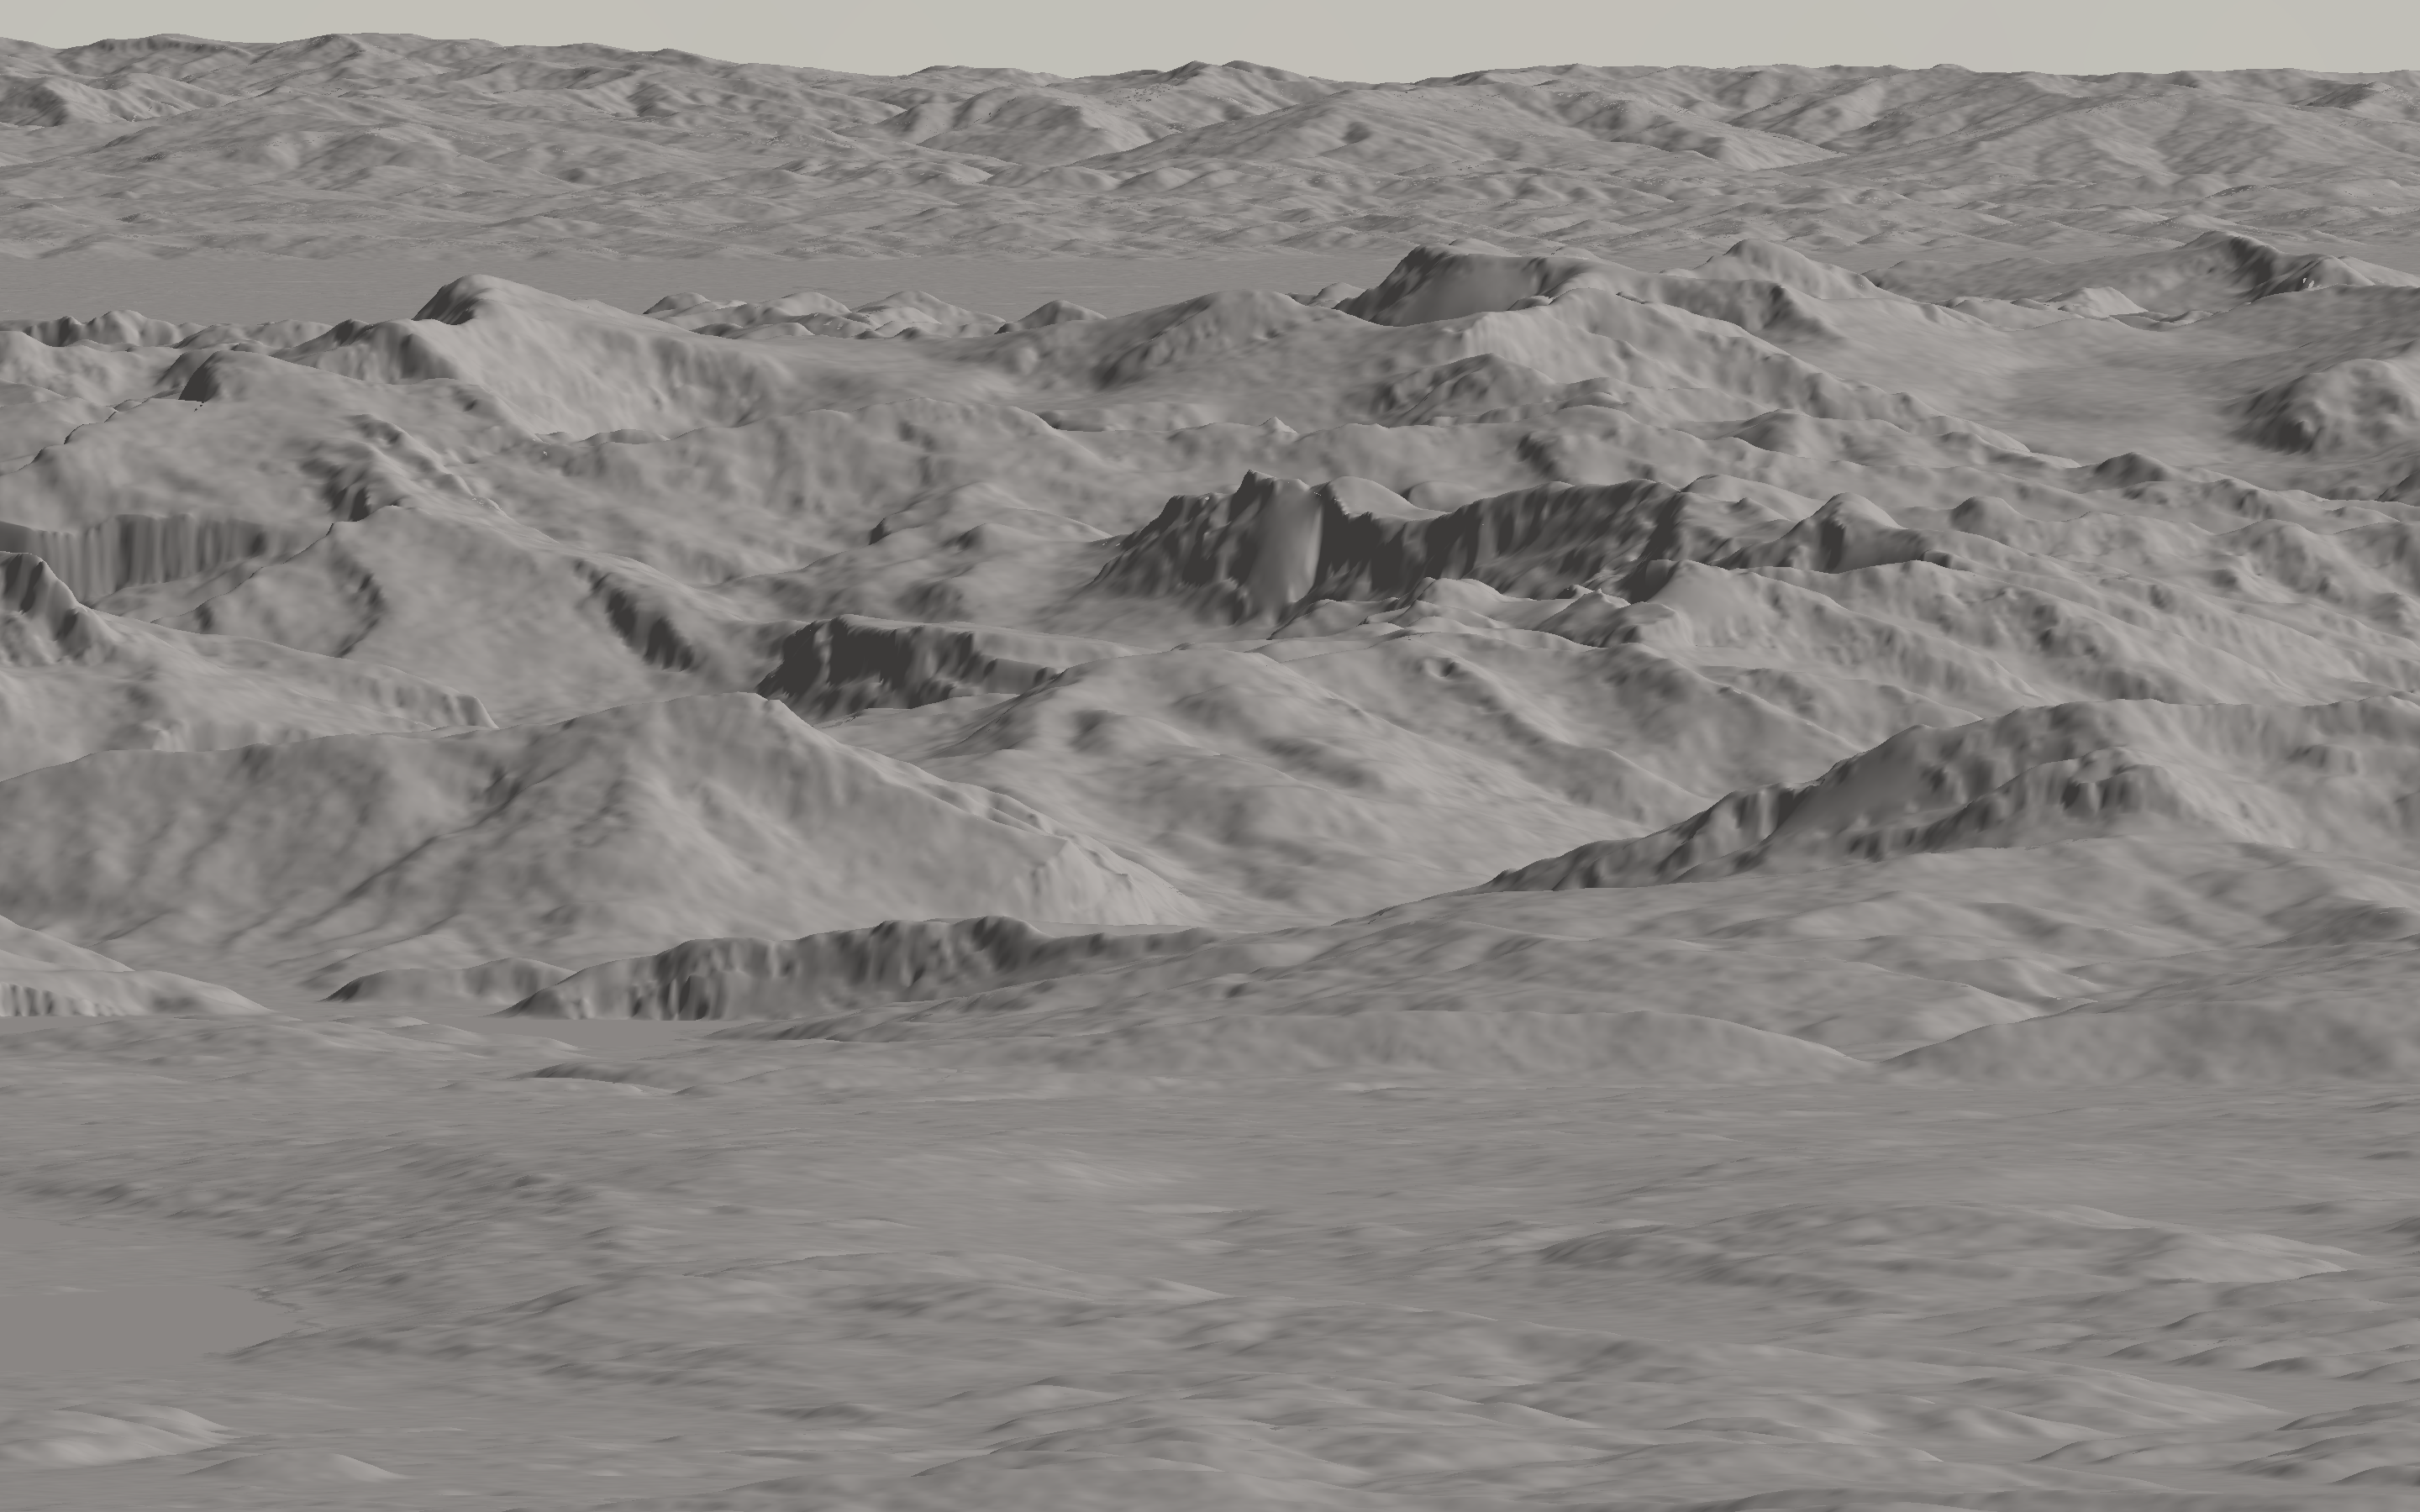
\includegraphics[width=0.4\textwidth]{results-accuracy-zoom-3-no-lod} }}
  \qquad
  \subfloat[\centering With LOD.]{{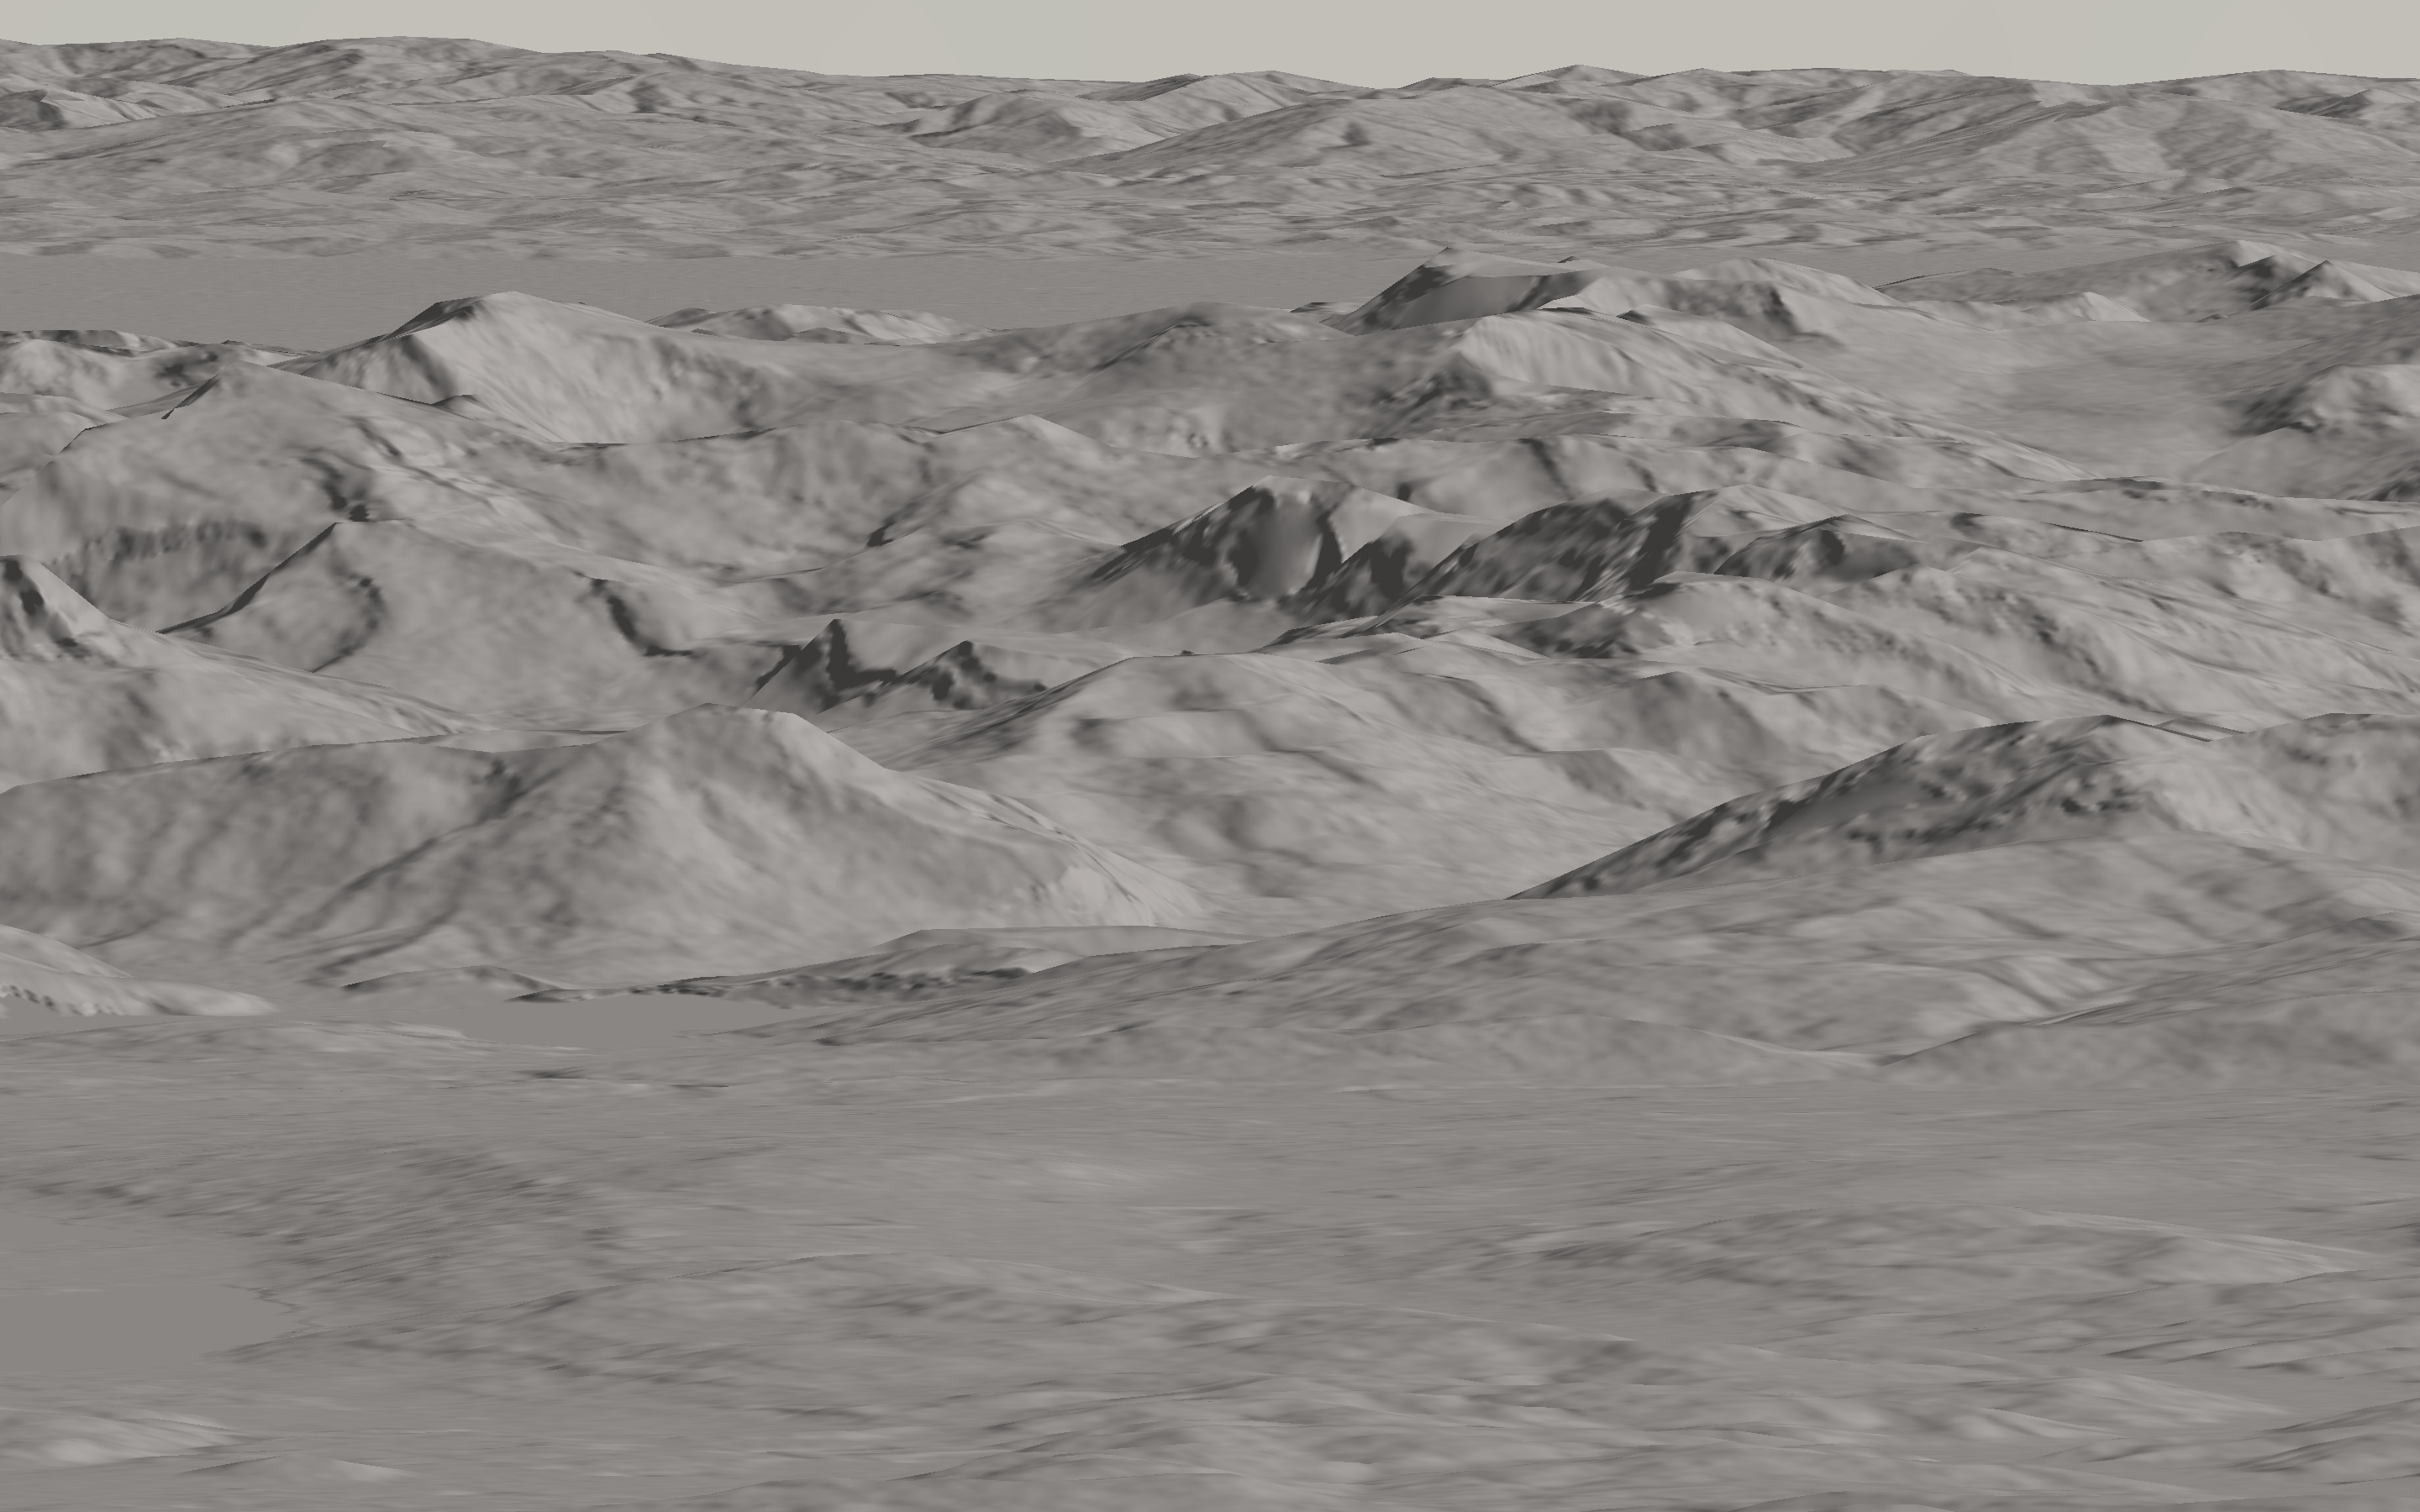
\includegraphics[width=0.4\textwidth]{results-accuracy-zoom-3-lod} }}
  \qquad
  \subfloat[\centering Absolute difference.]{{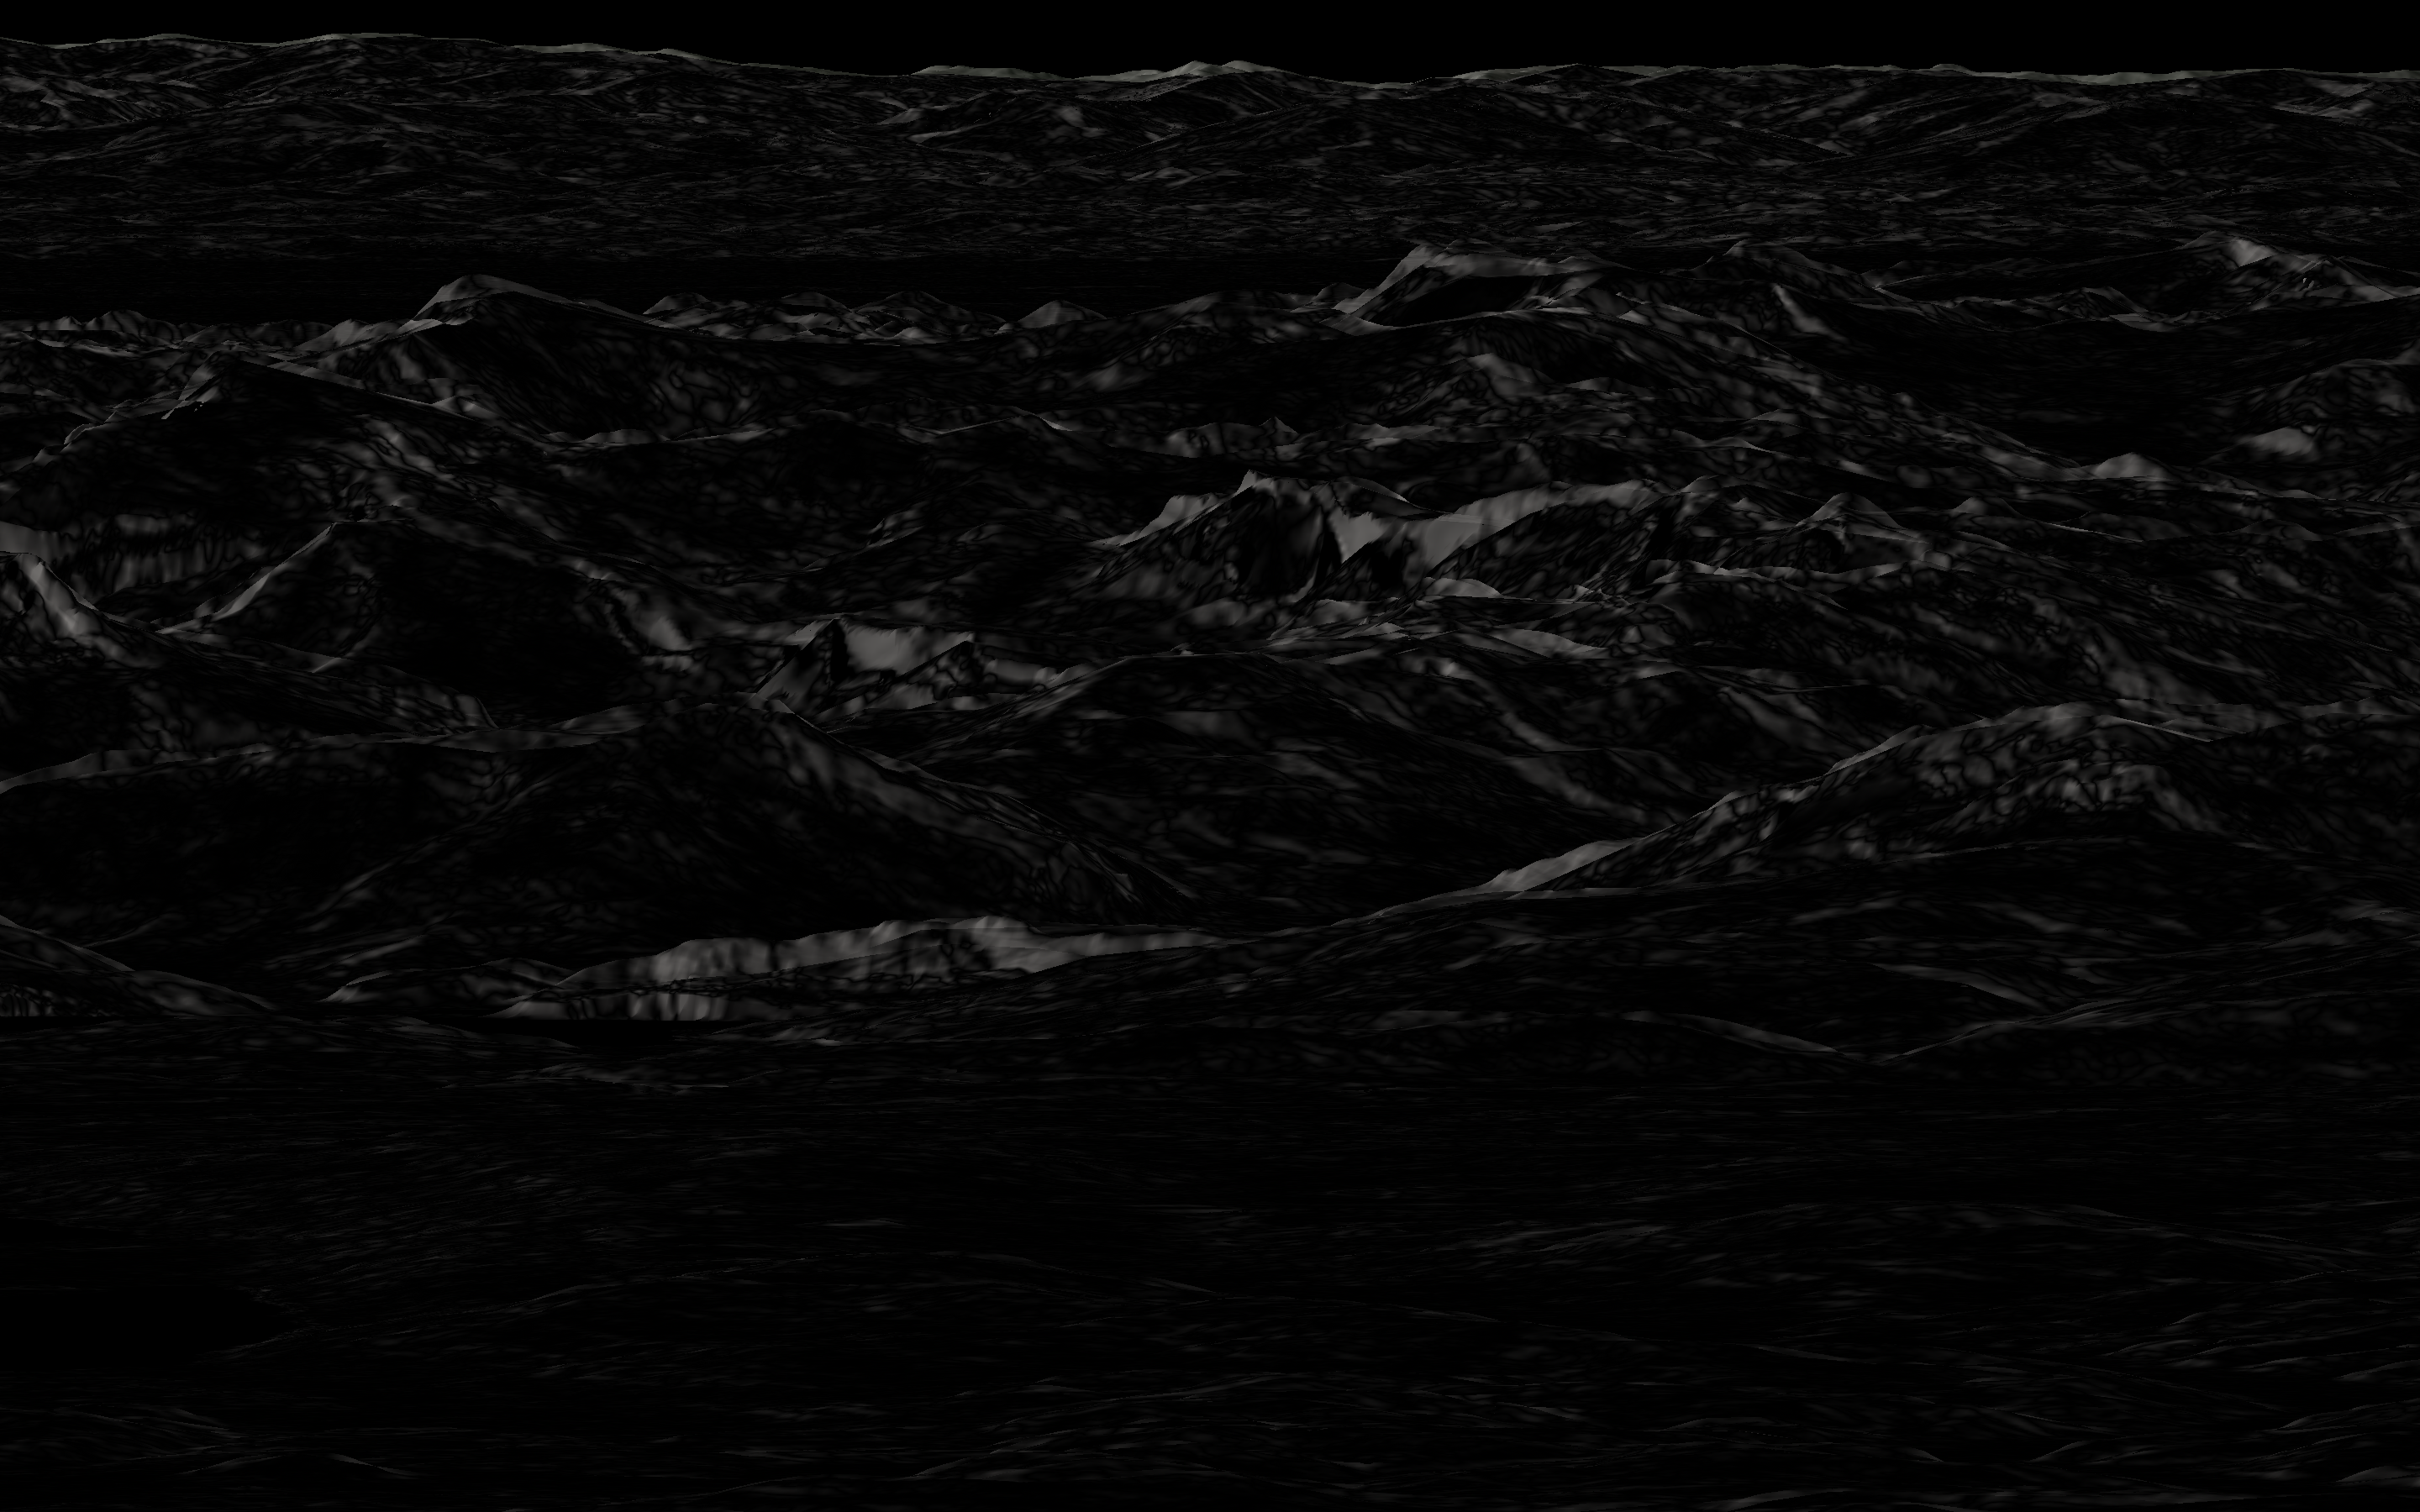
\includegraphics[width=0.4\textwidth]{results-accuracy-zoom-3-diff} }}
  \qquad
  \subfloat[\centering Absolute difference (binarised).]{{\includegraphics[width=0.4\textwidth]{results-accuracy-zoom-3-diff-bin} }}
  \caption{Screenshot showcasing the screenshot of a small section of the terrain with no LOD (a), with LOD (b),
  the absolute difference (c) between (a) and (b) and the binarised absolute difference (d) of (c). The FOV is set to $2^{\circ}$ and the computed RSME is 4.78.}\label{fig:results-zoom-3}
\end{figure}

\subsubsection{Low FOV Screenshot 4}
\begin{figure}[H]
  \centering
  \subfloat[\centering No LOD.]{{\includegraphics[width=0.4\textwidth]{results-accuracy-zoom-4-no-lod} }}
  \qquad
  \subfloat[\centering With LOD.]{{\includegraphics[width=0.4\textwidth]{results-accuracy-zoom-4-lod} }}
  \qquad
  \subfloat[\centering Absolute difference.]{{\includegraphics[width=0.4\textwidth]{results-accuracy-zoom-4-diff} }}
  \qquad
  \subfloat[\centering Absolute difference (binarised).]{{\includegraphics[width=0.4\textwidth]{results-accuracy-zoom-4-diff-bin} }}
  \caption{Screenshot showcasing the screenshot of a small section of the terrain with no LOD (a), with LOD (b),
  the absolute difference (c) between (a) and (b) and the binarised absolute difference (d) of (c). The FOV is set to $1^{\circ}$ and the computed RSME is 5.3.}\label{fig:results-zoom-4}
\end{figure}
\subsubsection{Low FOV Screenshot 5}
\begin{figure}[H]
  \centering
  \subfloat[\centering No LOD.]{{\includegraphics[width=0.4\textwidth]{results-accuracy-zoom-5-no-lod} }}
  \qquad
  \subfloat[\centering With LOD.]{{\includegraphics[width=0.4\textwidth]{results-accuracy-zoom-5-lod} }}
  \qquad
  \subfloat[\centering Absolute difference.]{{\includegraphics[width=0.4\textwidth]{results-accuracy-zoom-5-diff} }}
  \qquad
  \subfloat[\centering Absolute difference (binarised).]{{\includegraphics[width=0.4\textwidth]{results-accuracy-zoom-5-diff-bin} }}
  \caption{Screenshot showcasing the screenshot of a small section of the terrain with no LOD (a), with LOD (b),
  the absolute difference (c) between (a) and (b) and the binarised absolute difference (d) of (c). The FOV is set to $1^{\circ}$ and the computed RSME is 4.49.}\label{fig:results-zoom-5}
\end{figure}